% !TeX program = xelatex
% !TeX encoding = UTF-8
\input{setup.tex}

% Режим шаблона (должен быть включен один из трех)
\ВКРtrue
%\Практикаtrue
%\Курсоваяtrue

\newcommand{\Дисциплина}{<<Проектирование и архитектура программных систем>>}
\newcommand{\КодСпециальности}{09.03.04}
\newcommand{\Специальность}{Программная инженерия}
\newcommand{\Тема}{Бизнес-проект <<Программная реализация системы эвакуации маршрутов}
\newcommand{\ТемаВтораяСтрока}{для замкнутых пространств.>> Программная реализация и тестирование}
\newcommand{\ТемаТретьяСтрока}{алгоритмов динамической маршрутизации}
\newcommand{\ГдеПроводитсяПрактика}{АНО ДПО "УНЦИЯ"}
\newcommand{\РуководительПрактПредпр}{Лескова И. В.}
\newcommand{\ДолжнРуководительПрактПредпр}{президент}
\newcommand{\РуководительПрактУнивер}{Чаплыгин А. А.}
\newcommand{\ДолжнРуководительПрактУнивер}{к.т.н., доцент}
\newcommand{\Автор}{В. А. Старков}
\newcommand{\АвторРод}{Старкова В. А.}
\newcommand{\АвторПолностьюРод}{Старкова Вадима Артемовича}
\newcommand{\Шифр}{22-06-0111}
\newcommand{\Курс}{4 }
\newcommand{\Группа}{ПО-21б}
\newcommand{\Руководитель}{Р. А. Томакова}
\newcommand{\Нормоконтроль}{А. А. Чаплыгин}
\newcommand{\ЗавКаф}{А. В. Малышев}
\newcommand{\ДатаПриказа}{<<03>> апреля 2026~г.}
\newcommand{\НомерПриказа}{1584-с}
\newcommand{\СрокПредоставления}{<<09>> июня 2026~г.}

\begin{document}
\maketitle
\ifПрактика{}\else{
   \newpage
\begin{center}
\large\textbf{Минобрнауки России}

\large\textbf{Юго-Западный государственный университет}
\vskip 1em
\normalsize{Кафедра программной инженерии}
\vskip 1em
\ifВКР{
        \begin{flushright}
        \begin{tabular}{p{.4\textwidth}}
        \centrow УТВЕРЖДАЮ: \\
        \centrow Заведующий кафедрой \\
        \hrulefill \\
        \setarstrut{\footnotesize}
        \centrow\footnotesize{(подпись, инициалы, фамилия)}\\
        \restorearstrut
        «\underline{\hspace{1cm}}»
        \underline{\hspace{3cm}}
        20\underline{\hspace{1cm}} г.\\
        \end{tabular}
        \end{flushright}
        }\fi
\end{center}
\vspace{1em}
  \begin{center}
  \large
\ifВКР{
ЗАДАНИЕ НА ВЫПУСКНУЮ КВАЛИФИКАЦИОННУЮ РАБОТУ
  ПО ПРОГРАММЕ БАКАЛАВРИАТА}
  \else
ЗАДАНИЕ НА КУРСОВУЮ РАБОТУ (ПРОЕКТ)
\fi
\normalsize
  \end{center}
\vspace{1em}
{\parindent0pt
  Студента \АвторРод, шифр\ \Шифр, группа \Группа
  
1. Тема «\Тема\ \ТемаВтораяСтрока\ \ТемаТретьяСтрока»
\ifВКР{
утверждена приказом ректора ЮЗГУ от \ДатаПриказа\ № \НомерПриказа
}\fi.

2. Срок предоставления работы к защите \СрокПредоставления

3. Исходные данные для создания программной системы:

3.1. Перечень решаемых задач:}

\renewcommand\labelenumi{\theenumi)}

\begin{enumerate}
\item проанализировать предметную область навигации внутри зданий и определить требования к системе;
\item разработать архитектуру программного комплекса для построения маршрутов внутри здания с учетом этажности, переходов и ограничений на перемещение;
\item реализовать средства работы с навигационным графом, планами этажей, QR-навигацией и расписанием;
\item создать интерфейс пользователя и административные инструменты для редактирования карты, маршрутов и справочных данных;
\item предусмотреть поддержку режима чрезвычайной ситуации с построением эвакуационных маршрутов;
\item проверить корректность работы основных сценариев использования и подготовить материалы по результатам разработки.
\end{enumerate}

{\parindent0pt
  3.2. Входные данные и требуемые результаты для программы:}

\begin{enumerate}
\item Входными данными для программной системы являются: планы этажей в формате SVG, сведения о зданиях, этажах и навигационных узлах, навигационный граф, данные пользователей и их ролей, расписание занятий, параметры маршрутизации, а также состояние режима чрезвычайной ситуации.
\item Выходными данными для программной системы являются: построенный маршрут между выбранными точками, пошаговые инструкции перемещения, визуальное отображение маршрута на плане этажа, QR-данные для навигационных узлов, сведения о текущем расписании и эвакуационные маршруты при активации режима чрезвычайной ситуации.
\end{enumerate}

{\parindent0pt

  4. Содержание работы (по разделам):
  
  4.1. Введение.
  
4.2. Анализ предметной области: назначение систем построения эвакуационных
маршрутов в реальном времени для замкнутых пространств, пользовательские
роли, основные сценарии определения местоположения, особенности работы с
картой здания, QR-навигацией, заблокированными участками и режимом
чрезвычайной ситуации.
  
4.3. Техническое задание: основание для разработки, назначение системы
построения эвакуационных маршрутов, требования к авторизации, построению
маршрутов, отображению карты, QR-навигации, административным функциям,
режиму чрезвычайной ситуации и оформлению программной документации.

4.4. Технический проект: общая характеристика системы построения
эвакуационных маршрутов, обоснование выбора {.NET MAUI}, XAML и
SkiaSharp, описание архитектуры MVVM, моделей навигационного графа,
сервисного слоя, пользовательского интерфейса, алгоритма построения маршрута
и работы с локальными JSON-данными.

4.5. Рабочий проект: спецификация основных компонентов и классов приложения,
описание экранов пользователя и администратора, проверка сценариев
авторизации, выбора аудитории, построения маршрута, сканирования QR-кода,
редактирования карты и активации режима чрезвычайной ситуации.

4.6. Заключение.

4.7. Список использованных источников.

5. Перечень графического материала:

\списокПлакатов

\vskip 2em
\begin{tabular}{p{6.8cm}C{3.8cm}C{4.8cm}}
Руководитель \ifВКР{ВКР}\else работы (проекта) \fi & \lhrulefill{\fill} & \fillcenter\Руководитель\\
\setarstrut{\footnotesize}
& \footnotesize{(подпись, дата)} & \footnotesize{(инициалы, фамилия)}\\
\restorearstrut
Задание принял к исполнению & \lhrulefill{\fill} & \fillcenter\Автор\\
\setarstrut{\footnotesize}
& \footnotesize{(подпись, дата)} & \footnotesize{(инициалы, фамилия)}\\
\restorearstrut
\end{tabular}
}

\renewcommand\labelenumi{\theenumi.}

   \abstract{РЕФЕРАТ}

Объем работы равен \formbytotal{lastpage}{страниц}{е}{ам}{ам}. Работа содержит \formbytotal{figurecnt}{иллюстраци}{ю}{и}{й}, \formbytotal{tablecnt}{таблиц}{у}{ы}{}, \arabic{bibcount} библиографических источников и \formbytotal{числоПлакатов}{лист}{}{а}{ов} графического материала. Количество приложений~-- 2. Графический материал представлен в приложении А. Фрагменты исходного кода представлены в приложении Б.

Перечень ключевых слов: навигация, замкнутое пространство, эвакуационный маршрут, алгоритм Дейкстры, динамическая маршрутизация, навигационный граф, исключение узлов, межэтажный переход, чрезвычайная ситуация, кратчайший путь, QR-навигация, расписание, .NET MAUI, SkiaSharp, MVVM.

Объектом разработки является система построения эвакуационных маршрутов в реальном времени для замкнутых пространств, реализованная в виде кроссплатформенного приложения на платформе .NET MAUI.

Целью выпускной квалификационной работы является программная реализация и тестирование алгоритмов динамической маршрутизации, обеспечивающих построение оптимальных эвакуационных маршрутов с учётом динамически изменяющихся препятствий и режима чрезвычайной ситуации.

В ходе работы был проведён анализ алгоритмов поиска кратчайших путей на графах, разработаны структуры данных навигационного графа и механизмы перестроения маршрута в обход заблокированных узлов, реализованы алгоритм Дейкстры и алгоритм поиска ближайшего эвакуационного выхода.


Разработанная система позволяет формировать эвакуационные маршруты в реальном времени и служит основой для дальнейшего развития навигационных систем в замкнутых пространствах.

\selectlanguage{english}
\abstract{ABSTRACT}

The volume of work is \formbytotal{lastpage}{page}{}{s}{s}. The work contains \formbytotal{figurecnt}{illustration}{}{s}{s}, \formbytotal{tablecnt}{table}{}{s}{s}, \arabic{bibcount} bibliographic sources and \formbytotal{числоПлакатов}{sheet}{}{s}{s} of graphic material. The number of applications is 2. The graphic material is presented in Annex~A. Source code fragments are presented in Annex~B.

List of keywords: navigation, enclosed space, evacuation route, Dijkstra’s algorithm, dynamic routing, navigation graph, node exclusion, inter-floor transition, emergency situation, shortest path, QR navigation, schedule, .NET MAUI, SkiaSharp, MVVM.

The subject of this development is a system for constructing real-time evacuation routes for enclosed spaces, implemented as a cross-platform application on the .NET MAUI platform.

The goal of this final qualification project is the software implementation and testing of dynamic routing algorithms that ensure the construction of optimal evacuation routes, taking into account dynamically changing obstacles and emergency conditions.

During the project, an analysis of shortest-path search algorithms on graphs was conducted; data structures for the navigation graph and mechanisms for rerouting around blocked nodes were developed; and Dijkstra’s algorithm and the nearest-exit search algorithm were implemented.

The developed system allows for the generation of evacuation routes in real time and serves as a foundation for the further development of navigation systems in enclosed spaces.
\selectlanguage{russian}
}\fi
\tableofcontents
\section*{ОБОЗНАЧЕНИЯ И СОКРАЩЕНИЯ}

API -- программный интерфейс приложения (Application Programming Interface).

C\# -- язык программирования, используемый для реализации логики приложения.

JSON (JavaScript Object Notation) -- текстовый формат обмена и хранения структурированных данных.

MVVM (Model--View--ViewModel) -- архитектурный шаблон, разделяющий модель данных, пользовательский интерфейс и модель представления.

QR-код -- двумерный штрихкод, используемый для быстрого определения точки на карте.

UI (User Interface) -- пользовательский интерфейс.

UX (User Experience) -- пользовательский опыт.

XAML (Extensible Application Markup Language) -- язык разметки пользовательского интерфейса в приложениях .NET MAUI.

Граф -- структура данных, состоящая из узлов и рёбер, используемая для представления помещений, переходов и маршрутов.

ИС -- информационная система.

ПО -- программное обеспечение.

ТЗ -- техническое задание.

ТП -- технический проект.

ЧС -- чрезвычайная ситуация.

SVG (Scalable Vector Graphics) -- формат векторной графики, используемый для представления планов этажей.

UML (Unified Modelling Language) -- язык графического описания для объектного моделирования в области разработки программного обеспечения.

% !TeX root = mainstarkov.tex
% !TeX program = xelatex
% !TeX encoding = UTF-8
\newpage
\section*{РЕЗЮМЕ СТАРТАП-ПРОЕКТА}
\addcontentsline{toc}{section}{РЕЗЮМЕ СТАРТАП-ПРОЕКТА}

Название: «\Тема\ \ТемаВтораяСтрока\ \ТемаТретьяСтрока». Проект представляет собой кроссплатформенное приложение IndoorNav, предназначенное для навигации внутри зданий и автоматического построения эвакуационных маршрутов в чрезвычайных ситуациях. Система обеспечивает построение кратчайших маршрутов между помещениями, поиск ближайшего эвакуационного выхода, динамическое перестроение маршрута при блокировке участков пути, а также реализацию комплекса мер по обеспечению безопасности пользователей в режиме ЧС.

Ключевые возможности системы включают:
\begin{enumerate}
\item Построение кратчайших маршрутов между произвольными точками внутри здания с учётом межэтажных переходов и длин рёбер навигационного графа.

\item Автоматический поиск ближайшего эвакуационного выхода при активации режима чрезвычайной ситуации.

\item Перестроение маршрута в обход заблокированных участков без повторной загрузки графа.

\item Определение стартовой точки пользователя путём сканирования QR-кодов со стены здания.

\item Определение аудитории студента по расписанию и построение пути к выходу после её подтверждения.

\item Встроенный редактор графа, позволяющий администратору формировать карту здания без перекомпиляции приложения.
\end{enumerate}

Разработанная система оптимизирует процесс эвакуации из замкнутых пространств, повышая безопасность пользователей за счёт оперативного построения оптимальных маршрутов к выходам с учётом заблокированных проходов.

Актуальность проекта обусловлена требованиями обеспечения безопасности людей в зданиях с большим количеством помещений и сложной планировкой. Бумажный план эвакуации статичен и не учитывает блокировку отдельных участков, что в условиях чрезвычайной ситуации может привести к выбору неоптимального или недоступного маршрута — цифровая система подобной ошибки не допускает.

Целью разработки является создание системы построения эвакуационных маршрутов в реальном времени, обеспечивающей:
\begin{itemize}
\item оперативное построение кратчайших маршрутов до ближайших выходов с учётом текущей обстановки;
\item динамическое изменение маршрута при блокировке участков пути;
\item работу на мобильных устройствах и настольных компьютерах;
\item возможность масштабирования на здания с различной планировкой и этажности.
\end{itemize}

Отличительные особенности разработанной системы по сравнению с существующими решениями:
\begin{enumerate}
\item Алгоритм Дейкстры с возможностью динамического исключения узлов, позволяющий перестраивать маршрут без модификации исходного графа.

\item Кроссплатформенная реализация на базе .NET MAUI с поддержкой Android, iOS и Windows.

\item Полная автономность: данные хранятся локально, потеря сети не прерывает навигацию.

\item Редактор карты для администратора, позволяющий формировать навигационный граф поверх плана этажа.

\item Интеграция с расписанием занятий для автоматического определения местоположения студента при активации ЧС.
\end{enumerate}

В системе реализованы алгоритмы маршрутизации (Дейкстра с исключением узлов, поиск ближайшего выхода), сервис управления режимом ЧС, аутентификация с разделением ролей (администратор, студент, гость), управление расписанием и позиционирование по QR-кодам.

Идея создания проекта возникла в 2025 году в связи с необходимостью обеспечения безопасной и оперативной эвакуации в зданиях университета. Разработка системы была начата в 2025 году и завершена в 2026 году в рамках выполнения выпускной квалификационной работы.

Бизнес-цели:
\begin{enumerate}
\item Внедрение системы навигации в зданиях университета для повышения безопасности студентов и сотрудников при чрезвычайных ситуациях.

\item Масштабирование системы для использования в зданиях различного назначения: образовательные учреждения, бизнес-центры, торговые комплексы.

\item Интеграция с системами пожарной безопасности и оповещения для автоматической активации режима ЧС.

\item Добавление push-уведомлений о чрезвычайных ситуациях и голосовые подсказки при навигации.

\item Ускорение процесса эвакуации за счёт автоматического определения местоположения пользователя.
\end{enumerate}

% !TeX root = mainstarkov.tex
% !TeX program = xelatex
% !TeX encoding = UTF-8
\section*{ВВЕДЕНИЕ}
\addcontentsline{toc}{section}{ВВЕДЕНИЕ}

Современные системы навигации в замкнутых пространствах требуют не только точного построения маршрутов, но и высокой производительности алгоритмов поиска пути, особенно в условиях динамически изменяющейся обстановки. В чрезвычайных ситуациях, когда определённые участки маршрута могут стать недоступными, система должна за миллисекунды перестроить оптимальный путь до ближайшего безопасного выхода.

Традиционные планы эвакуации решают только часть этой задачи. Они показывают общую схему движения, но остаются статичными: план не определяет местоположение конкретного пользователя, не учитывает заблокированный коридор и не перестраивает путь при изменении обстановки. При этом требования к эвакуационным путям и пожарной безопасности закреплены в нормативных документах, а значит программная система должна не подменять эти требования, а дополнять их прикладным механизмом построения маршрута.

В основе такой системы лежит представление здания в виде графа. Помещения, лестницы, лифты, выходы, QR-якоря и промежуточные точки маршрута рассматриваются как узлы, а допустимые переходы между ними – как рёбра. Это позволяет применять алгоритмы поиска кратчайшего пути, в том числе алгоритм Дейкстры, и учитывать дополнительные условия: смену этажа, недоступность отдельных участков, выбор ближайшего безопасного выхода. Теоретическая база подобных задач опирается на методы работы с графами и алгоритмы построения маршрутов.

Актуальность работы определяется необходимостью обеспечить надёжное и быстрое построение эвакуационных маршрутов в реальном времени. Алгоритмы маршрутизации должны обрабатывать графы с сотнями узлов и рёбер, учитывать межэтажные переходы, адаптироваться к изменениям в графе и гарантировать нахождение оптимального пути при наличии решения. Согласно критериям качества программного обеспечения по ГОСТ Р ИСО/МЭК 25010, в наибольшей степени проявляются характеристики функциональной пригодности (корректность маршрутизации), эффективности по производительности (время построения маршрута) и надёжности (устойчивость к блокировкам). Поэтому при реализации недостаточно только запрограммировать алгоритм: необходимо определить подходящие структуры данных, обеспечить обработку динамических ограничений и верифицировать корректность тестами.

\emph{Цель настоящей работы} -- реализовать и протестировать алгоритмы динамической маршрутизации для системы построения эвакуационных маршрутов, обеспечивающие построение оптимальных путей с учётом заблокированных участков и режима чрезвычайной ситуации.

Для достижения поставленной цели необходимо решить \emph{следующие задачи}:
\begin{itemize}
\item изучить существующие алгоритмы поиска кратчайших путей на графах;
\item спроектировать структуры данных для эффективного хранения и обработки навигационного графа;
\item реализовать алгоритм Дейкстры с поддержкой динамического исключения узлов;
\item реализовать алгоритм поиска ближайшего эвакуационного выхода с учётом текущего положения;
\item построить механизм формирования множества исключаемых узлов для перестроения маршрута;
\item провести модульное и системное тестирование алгоритмов на разных сценариях;
\item оценить быстродействие и правильность работы алгоритмов.
\end{itemize}

\emph{Структура и объём работы} -- Отчет состоит из введения, 4 разделов
основной части, заключения, списка использованных источников, приложений и графического материала на отдельных листах. Объём текста выпускной
квалификационной работы составляет \formbytotal{lastpage}{страниц}{у}{ы}{}.

\emph{Во введении} сформулирована цель работы, поставлены задачи разработки, описана структура работы, приведено краткое содержание каждого из разделов.

\emph{В первом разделе} на стадии анализа предметной области рассмотрены алгоритмы поиска кратчайших путей на графах, проведён их сравнительный анализ, рассмотрены способы представления графа в памяти и проанализированы существующие реализации систем indoor-навигации.

\emph{Во втором разделе} на стадии технического задания приводятся требования к разрабатываемой программной системе.

\emph{В третьем разделе} на стадии технического проектирования представлены проектные решения для программной системы.

\emph{В четвертом разделе} приводится список функций, классов и их методов, использованных при разработке программной системы, производится тестирование разработанной программной системы

В заключении излагаются основные результаты работы, полученные в ходе разработки.

В приложении А представлен графический материал.
В приложении Б представлены фрагменты исходного кода. 
% !TeX root = mainstarkov.tex
% !TeX program = xelatex
% !TeX encoding = UTF-8
\section{Анализ}

\subsection{Предметная область алгоритмов поиска путей}

Задача построения оптимального маршрута в замкнутом пространстве сводится к поиску кратчайшего пути на взвешенном неориентированном графе. Вершины графа соответствуют помещениям, коридорам, лестничным площадкам и лифтам, а рёбра -- проходам между ними с весами, пропорциональными расстоянию или времени прохождения. Такая модель является стандартной для систем indoor-навигации \cite{mongush2017} и опирается на классическую теорию графов \cite{zhang2015}.

В отличие от наружной навигации, где маршруты строятся по дорожной сети с относительно простой топологией, навигация внутри здания характеризуется многоэтажностью, наличием переходов между этажами с различным расстоянием (лестницы, лифты), а также возможностью динамического изменения проходимости участков. При возникновении чрезвычайной ситуации определённые проходы могут стать заблокированными, что требует немедленного перестроения маршрута. Существующие подходы к навигации внутри зданий охватывают как методы определения положения пользователя~-- по Bluetooth, Wi-Fi, компьютерному зрению, QR-меткам \cite{grinyak2018,singh2021,tomazic2021}, так и построение и сопровождение самого маршрута \cite{kulikov2021,landau2020,rubio2021,ohotichenko2021}; настоящая работа сосредоточена на втором. Особую роль навигация играет при эвакуации: требования к путям и выходам закреплены в нормативных документах \cite{fz123,sp113130}, информационные технологии всё активнее применяются для повышения пожарной безопасности зданий \cite{gusarova2023}, тогда как бумажные планы эвакуации статичны и требуют времени на изучение \cite{samoshin2026}.

Предметная область алгоритмов маршрутизации в системах эвакуации включает следующие ключевые задачи:
\begin{itemize}
\item поиск кратчайшего пути между двумя заданными точками внутри здания;
\item учёт весов рёбер, отражающих реальное расстояние или время прохождения;
\item динамическое исключение заблокированных узлов без модификации исходного графа;
\item поиск кратчайшего пути до ближайшего эвакуационного выхода из текущего положения;
\item обработка межэтажных переходов с учетом веса ребра;
\item обеспечение производительности, достаточной для работы в реальном времени.
\end{itemize}

\subsection{Обзор алгоритмов поиска кратчайших путей}

Для решения задачи поиска кратчайших путей на графах разработан ряд классических алгоритмов, каждый из которых имеет свои области применения, преимущества и ограничения. Ниже рассмотрены основные алгоритмы, применимые к задаче эвакуационной маршрутизации \cite{amelichev2022,isaev2023,levitin}.

\textbf{1. Алгоритм Дейкстры} \cite{dijkstra,mirahadi2021} находит кратчайшие пути от одной вершины до всех остальных в графе с неотрицательными весами рёбер. Алгоритм работает следующим образом: на каждом шаге выбирается непосещённая вершина с минимальным текущим расстоянием, после чего выполняется релаксация всех исходящих из неё рёбер. Сложность алгоритма составляет $O((V + E) \log V)$ при использовании бинарной кучи или $O(E + V \log V)$ с кучей Фибоначчи, где $V$ -- число вершин, $E$ -- число рёбер. Алгоритм гарантирует оптимальность решения для графов с неотрицательными весами и является одним из наиболее изученных и надёжных алгоритмов поиска путей.

Достоинства алгоритма Дейкстры: гарантия оптимальности при неотрицательных весах; эффективная работа на разреженных графах; возможность остановки при достижении целевой вершины; простота модификации для учёта динамических ограничений; широкая распространённость и наличие проверенных реализаций.

Недостатки: не работает с отрицательными весами рёбер; требует полной инициализации расстояний для всех вершин; не учитывает направление к цели (в отличие от эвристических алгоритмов).

\textbf{2. Алгоритм A*} является расширением алгоритма Дейкстры с использованием эвристической функции $h(v)$, оценивающей расстояние от вершины $v$ до цели. Функция приоритета имеет вид $f(v) = g(v) + h(v)$, где $g(v)$ -- текущее кратчайшее расстояние от старта, $h(v)$ -- эвристическая оценка расстояния до цели. При допустимой эвристике ($h(v) \leq$ реальное расстояние) A* гарантирует оптимальность и обычно посещает меньше вершин, чем Дейкстра.

Достоинства A*: значительное сокращение области поиска при подходящей эвристике; оптимальность при допустимой эвристике; широкое применение в игровой индустрии и робототехнике.

Недостатки: требует разработки эвристической функции, что затруднительно для indoor-графов с произвольной топологией; эвристика на основе евклидова расстояния может быть неточной из-за стен и непроходимых участков; при динамическом исключении узлов эвристика может стать недопустимой; производительность сильно зависит от качества эвристики.

\textbf{3. Алгоритм Флойда--Уоршелла} находит кратчайшие пути между всеми парами вершин за $O(V^3)$. Алгоритм последовательно рассматривает каждую вершину как промежуточную и обновляет расстояния между всеми парами. Результат хранится в матрице расстояний, что позволяет получать путь между любыми двумя вершинами за $O(1)$.

Достоинства: полная матрица кратчайших путей; простота реализации; работа с отрицательными весами (без отрицательных циклов).

Недостатки: кубическая сложность делает алгоритм неприменимым для графов с сотнями вершин; при изменении одного ребра требуется полный пересчёт; высокое потребление памяти ($O(V^2)$); не подходит для динамической маршрутизации.

\textbf{4. Поиск в ширину (BFS)} обходит граф уровнями от стартовой вершины, гарантируя нахождение кратчайшего пути в количестве рёбер. BFS работает за $O(V + E)$ и является оптимальным для невзвешенных графов.

Достоинства: линейная сложность; простота реализации; нахождение кратчайшего пути по числу рёбер.

Недостатки: не учитывает веса рёбер, что делает его непригодным для графов с различной длиной проходов; не различает короткие коридоры и длинные лестницы; не применим для оптимизации по расстоянию или времени.

\textbf{5. Алгоритм Беллмана--Форда} находит кратчайшие пути от одной вершины до всех остальных, допуская отрицательные веса рёбер. Сложность составляет $O(V \cdot E)$. Алгоритм выполняет $V - 1$ итераций релаксации всех рёбер.

Достоинства: поддержка отрицательных весов; обнаружение отрицательных циклов.

Недостатки: значительно медленнее Дейкстры ($O(V \cdot E)$ vs $O((V+E)\log V)$); отрицательные веса не требуются в задаче навигации; избыточность для рассматриваемой задачи.

\subsection{Сравнительный анализ алгоритмов}

Сравнение рассмотренных алгоритмов по ключевым критериям приведены в таблицах~\ref{algcompare:table1} и \ref{algcompare2:table1}.

\begin{xltabular}{\textwidth}{|X|c|c|c|}
\caption{Сравнение алгоритмов Дейкстры, A* и Флойда\label{algcompare:table1}}\\ \hline
\centrow Критерий & \centrow Дейкстра & \centrow A* & \centrow Флойд \\ \hline
\endfirsthead
\continuecaption{Продолжение таблицы \ref{algcompare:table1}}
\centrow Критерий & \centrow Дейкстра & \centrow A* & \centrow Флойд \\ \hline
\finishhead
Сложность & $O((V{+}E)\log V)$ & $O((V{+}E)\log V)$ & $O(V^3)$ \\ \hline
Оптимальность & Да & Да* & Да \\ \hline
Отриц.\ веса & Нет & Нет & Да \\ \hline
Динамич.\ искл.\ узлов & Да & Затруднено & Нет \\ \hline
Требует эвристику & Нет & Да & Нет \\ \hline
Память & $O(V{+}E)$ & $O(V{+}E)$ & $O(V^2)$ \\ \hline
Пересчёт при изменении & Полный & Полный & Полный
\end{xltabular}

\begin{xltabular}{\textwidth}{|X|c|c|}
\caption{Сравнение алгоритмов BFS и Беллмана--Форда\label{algcompare2:table1}}\\ \hline
\centrow Критерий & \centrow BFS & \centrow Беллман--Форд \\ \hline
\endfirsthead
\continuecaption{Продолжение таблицы \ref{algcompare2:table1}}
\centrow Критерий & \centrow BFS & \centrow Беллман--Форд \\ \hline
\finishhead
Сложность & $O(V{+}E)$ & $O(V \cdot E)$ \\ \hline
Оптимальность & По рёбрам & Да \\ \hline
Отриц.\ веса & Нет & Да \\ \hline
Динамич.\ искл.\ узлов & Да & Да \\ \hline
Требует эвристику & Нет & Нет \\ \hline
Память & $O(V{+}E)$ & $O(V{+}E)$ \\ \hline
Пересчёт при изменении & Полный & Полный
\end{xltabular}
\subsection{Представление графа в памяти}

Граф можно хранить двумя основными способами~-- матрицей смежности или списком смежности; выбор заметно влияет на расход памяти и скорость работы алгоритма.

\emph{Матрица смежности}~-- это таблица $V \times V$, где на пересечении строки $i$ и столбца $j$ стоит длина ребра между вершинами $i$ и $j$ (или признак его отсутствия). Проверка наличия ребра выполняется за $O(1)$, но память расходуется как $O(V^2)$ независимо от числа рёбер, а перебор соседей одной вершины стоит $O(V)$.

\emph{Список смежности} хранит для каждой вершины перечень её соседей с длинами. Память при этом~-- $O(V + E)$, а соседи перебираются ровно за их количество.

Граф здания разрежен: у каждого узла обычно два-четыре соседа, поэтому $E \approx 2{-}3V$. Сравнение двух представлений для такого случая приведено в таблице~\ref{graphrepr:table}.

\begin{xltabular}{\textwidth}{|X|c|c|}
	\caption{Сравнение способов представления графа\label{graphrepr:table}}\\ \hline
	\centrow Характеристика & \centrow Матрица & \centrow Список \\ \hline
	\endfirsthead
	\continuecaption{Продолжение таблицы \ref{graphrepr:table}}
	\centrow Характеристика & \centrow Матрица & \centrow Список \\ \hline
	\finishhead
	Память & $O(V^2)$ & $O(V{+}E)$ \\ \hline
	Перебор соседей вершины & $O(V)$ & $O(\deg v)$ \\ \hline
	Проверка наличия ребра & $O(1)$ & $O(\deg v)$ \\ \hline
	Подходит для разреженных графов & Нет & Да
\end{xltabular}

Алгоритм Дейкстры на каждом шаге перебирает соседей текущей вершины, а проверка отдельных рёбер ему почти не нужна. Поэтому для разреженного графа здания выбран список смежности: он экономит память (на 586 узлах матрица заняла бы около 340~тысяч ячеек против примерно 2,4~тысячи связей в списке) и ускоряет основной цикл алгоритма.

\subsection{Обоснование выбора алгоритма Дейкстры}

Для системы построения эвакуационных маршрутов выбран алгоритм Дейкстры по следующим причинам:

\begin{itemize}
\item эффективная работа на разреженных графах, характерных для планов зданий ($E \approx 2-3V$), в отличие от алгоритма Флойда--Уоршелла, требующего $O(V^3)$;
\item возможность модификации для исключения заблокированных узлов без полного пересчёта структуры графа -- достаточно передать множество исключений как параметр;
\item простота реализации с использованием стандартных структур данных .NET (\texttt{SortedSet}, \texttt{Dictionary}, \texttt{HashSet});
\item достаточная производительность для графов с сотнями узлов (целевое время $<200$ мс);
\item отсутствие необходимости в эвристической функции, разработка которой затруднена для indoor-графов с произвольной топологией;
\item возможность остановки при достижении целевой вершины без обработки всего графа.
\end{itemize}

Алгоритм A* не выбран, поскольку для навигационного графа здания с произвольной конфигурацией стен и переходов трудно построить допустимую эвристику. Евклидово расстояние не учитывает непроходимые стены, а манхэттенское расстояние не соответствует реальной топологии коридоров. Кроме того, при динамическом исключении узлов эвристика может стать недопустимой, что нарушит гарантию оптимальности.

\subsection{Особенности применения алгоритма Дейкстры к эвакуационной маршрутизации}

Применение алгоритма Дейкстры к задаче эвакуации требует учёта следующих специфических требований, отличающих данную задачу от стандартного поиска кратчайшего пути.

\textbf{Динамическое исключение узлов.} В режиме чрезвычайной ситуации или при обходе препятствий определённые узлы графа (проходы, двери, лестницы) могут стать недоступными. Алгоритм должен исключать такие узлы из рассмотрения без модификации исходного графа. Это реализуется путём передачи множества исключённых идентификаторов как параметра алгоритма. При релаксации рёбер алгоритм проверяет, не находится ли соседняя вершина в множестве исключений, и пропускает её. Конечная вершина маршрута никогда не исключается, даже если она присутствует в множестве \cite{mirahadi2020,zhangfire2019}.

\textbf{Вес межэтажных переходов.} Переход между этажами через лестницу или лифт имеет более большой вес ребра по сравнению с горизонтальным перемещением по коридору. Для межэтажных переходов назначается фиксированный вес, отражающий затраты времени на подъём/спуск. Данный подход позволяет алгоритму предпочитать горизонтальные маршруты, если они незначительно длиннее маршрута со сменой этажа \cite{gravit2019}.

\textbf{Поиск до ближайшего выхода.} Вместо поиска пути до заданной цели требуется найти кратчайший путь до любого из узлов, помеченных как эвакуационный выход. Это достигается запуском алгоритма Дейкстры от текущего положения пользователя с последующим сравнением расстояний до всех доступных выходов. Выбирается выход с минимальной суммарной стоимостью пути. Приоритет отдаётся выходам в том же здании, что и текущее положение пользователя \cite{han2020,yen2021}.

\textbf{Обработка отсутствия пути.} Если после завершения алгоритма расстояние до целевой вершины остаётся бесконечным (вершина недостижима), алгоритм должен возвращать пустой список, а не генерировать исключение. Это важно для устойчивости системы: при полной блокировке пути приложение должно корректно информировать пользователя, а не завершаться аварийно \cite{deng2021}.

\subsection{Анализ существующих реализаций}

На рынке существует ряд библиотек и фреймворков, предоставляющих реализацию алгоритмов поиска кратчайших путей. Готовые коммерческие платформы indoor-навигации \cite{navigineSdk,situmDocs,mappedinDocs,twogisFloors,mapstedOfficial} предоставляют навигацию внутри зданий как услугу, но они закрыты, требуют подписки и не дают доступа к реализации алгоритма маршрутизации. Поэтому ниже рассмотрены открытые алгоритмические библиотеки, наиболее известные из них.

\textbf{1. NetworkX} (Python) -- библиотека для работы с графами, предоставляющая реализации алгоритмов Дейкстры, A*, Флойда--Уоршелла и множества других. Широко используется в научных исследованиях и прототипировании. Однако библиотека написана на Python и не подходит для интеграции в .NET-приложение.

\textbf{2. QuickGraph} (C\#) -- библиотека графовых алгоритмов для .NET, предоставляющая реализации Дейкстры, A* и других алгоритмов. Поддерживает ориентированные и неориентированные графы с произвольными типами вершин. Недостатком является отсутствие поддержки динамического исключения узлов из коробки, а также отсутствие поддержки .NET MAUI.

\textbf{3. Boost.Graph} (C++) -- мощная библиотека графовых алгоритмов из набора Boost. Предоставляет высокопроизводительные реализации множества алгоритмов. Не подходит для .NET-приложения из-за языковых различий и сложности интеграции.

\textbf{4. Собственная реализация} -- разработка алгоритма Дейкстры на C\# с использованием стандартных коллекций .NET. Этот подход обеспечивает полный контроль над логикой алгоритма, возможность модификации для динамического исключения узлов, отсутствие внешних зависимостей и простоту отладки.

Для разрабатываемой системы выбрана собственная реализация, поскольку ни одна из существующих библиотек не предоставляет готовой поддержки динамического исключения узлов, необходимой для режима эвакуации. Кроме того, собственная реализация позволяет оптимизировать структуры данных под конкретную задачу и избежать лишних зависимостей.

\subsection{Выводы по разделу}

Проведённый анализ показывает, что алгоритм Дейкстры с использованием современных структур данных наилучшим образом соответствует требованиям задачи динамической эвакуационной маршрутизации. Его модификация для работы с динамически исключаемыми узлами и поиском ближайшего выхода позволяет создать надёжную основу для системы реального времени.

Ключевые результаты анализа:
\begin{itemize}
\item алгоритм Дейкстры обеспечивает оптимальность и достаточную производительность для графов зданий;
\item алгоритм A* не подходит из-за сложности построения допустимой эвристики для indoor-графов;
\item алгоритм Флойда--Уоршелла неприменим из-за кубической сложности;
\item BFS не учитывает веса рёбер;
\item собственная реализация предпочтительнее использования сторонних библиотек из-за необходимости поддержки динамического исключения узлов.
\end{itemize}

% !TeX root = mainstarkov.tex
% !TeX program = xelatex
% !TeX encoding = UTF-8
\section{Техническое задание}

\subsection{Основание для разработки}

Основанием для разработки является задание на выпускную квалификационную работу по теме «\Тема\ \ТемаВтораяСтрока\ \ТемаТретьяСтрока». Разработка ведётся в соответствии с ГОСТ 19.102-77 \cite{gost19102} (стадии разработки) и ГОСТ 19.201-78 \cite{gost19201} (требования к техническому заданию).

Объектом разработки является алгоритмическое ядро системы построения эвакуационных маршрутов в реальном времени для замкнутых пространств, реализованное в виде модуля динамической маршрутизации приложения IndoorNav.

\subsection{Назначение разработки}

\textbf{Функциональное назначение.} Модуль динамической маршрутизации предназначен для:
\begin{itemize}
\item построения кратчайших маршрутов между точками внутри здания с учётом весов рёбер;
\item поиска ближайшего эвакуационного выхода из текущего положения пользователя;
\item динамического перестроения маршрута при блокировке участков пути;
\item обработки межэтажных переходов;
\item восстановления последовательности узлов маршрута для навигации пользователя.
\end{itemize}

\textbf{Эксплуатационное назначение.} Модуль предназначен для использования в составе кроссплатформенного приложения IndoorNav на мобильных устройствах (Android, iOS) и настольных компьютерах (Windows). В штатном режиме модуль обеспечивает построение маршрутов между помещениями; в режиме ЧС -- автоматическое построение эвакуационного маршрута до ближайшего безопасного выхода.

\subsection{Требования к программной системе}

\subsubsection{Требования к данным программной системы}

Входными данными для модуля маршрутизации являются:
\begin{itemize}
\item навигационный граф в формате JSON (узлы, рёбра, здания, этажи);
\item идентификатор стартового узла (string);
\item идентификатор конечного узла (string);
\item множество исключённых узлов (\texttt{ISet<string>}, может быть пустым);
\item текущее состояние режима ЧС (флаг активности, идентификатор здания).
\end{itemize}

Выходными данными модуля являются:
\begin{itemize}
\item упорядоченный список узлов маршрута от старта до цели (\texttt{List<NavNode>});
\item пустой список при отсутствии пути;
\item суммарный вес маршрута (float);
\item путь до ближайшего эвакуационного выхода при активации ЧС.
\end{itemize}

Концептуальная модель данных модуля включает сущности: навигационный узел (NavNode), навигационное ребро (NavEdge), навигационный граф (NavGraph). Навигационный узел имеет тип (аудитория, коридор, лестница, лифт, выход, запасной выход, QR-якорь) и координаты на плане этажа. Навигационное ребро связывает два узла и имеет вес, вычисляемый как евклидово расстояние или штраф для межэтажных переходов.

\subsubsection{Требования к функциям программной системы}

\paragraph{Построение маршрута между точками.} Модуль должен:
\begin{itemize}
\item строить кратчайший путь между двумя заданными узлами графа по алгоритму Дейкстры;
\item учитывать веса рёбер при вычислении оптимального пути;
\item корректно обрабатывать ситуацию отсутствия пути (несвязный граф, полная блокировка);
\item обеспечивать время выполнения не более 200 мс для графа до 500 узлов и 1000 рёбер;
\item возвращать упорядоченный список узлов маршрута (начало → конец);
\item возвращать пустой список при совпадении стартового и конечного узла (путь из одного элемента);
\item возвращать пустой список при несуществующих идентификаторах узлов.
\end{itemize}

\paragraph{Динамическое исключение узлов.} Алгоритм должен поддерживать:
\begin{itemize}
\item передачу множества исключаемых узлов как параметра без модификации исходного графа;
\item игнорирование исключённых узлов при релаксации рёбер;
\item невозможность исключения конечного узла маршрута (даже если он в множестве);
\item корректную работу при последовательном добавлении исключений (повторный вызов);
\item использование \texttt{HashSet<string>} для проверки принадлежности множеству за $O(1)$;
\item возврат пустого результата при исключении всех возможных путей.
\end{itemize}

\paragraph{Поиск эвакуационного выхода.} Реализация должна обеспечивать:
\begin{itemize}
\item поиск кратчайшего пути до ближайшего узла с флагом \texttt{IsExit} или \texttt{IsEvacuationExit};
\item приоритет выходов в том же здании (\texttt{BuildingId}) при наличии нескольких корпусов;
\item автоматическое построение маршрута при активации режима ЧС;
\item возврат пустого результата при отсутствии доступных выходов;
\item учёт исключённых узлов и заблокированных участков при поиске выхода;
\item выбор выхода с минимальной суммой веса рёбер;
\item fallback на выходы других зданий при отсутствии выходов в текущем.
\end{itemize}

\paragraph{Обработка межэтажных переходов.} Система должна:
\begin{itemize}
\item корректно обрабатывать рёбра, соединяющие узлы разных этажей;
\item учитывать вес ребёр;
\item избегать ненужных смен этажей при наличии прямого горизонтального пути;
\item гарантировать достижимость любого этажа при отсутствии блокировок;
\item различать типы переходов: лестница вверх, лестница вниз, лифт;
\item формировать пошаговые инструкции при смене этажа.
\end{itemize}

\paragraph{Восстановление пути.} Алгоритм должен:
\begin{itemize}
\item сохранять предшественника для каждого достижимого узла;
\item восстанавливать полный путь от старта до цели обратным обходом;
\item возвращать путь в порядке от стартового узла к конечному;
\item корректно обрабатывать случай, когда старт и цель совпадают.
\end{itemize}

\subsubsection{Требования к структурам данных}

\paragraph{Представление графа.} Граф должен храниться в формате, обеспечивающем:
\begin{itemize}
\item быстрый доступ к узлу по идентификатору через словарь (\texttt{Dictionary<string, NavNode>});
\item хранение списка смежности для каждого узла (\texttt{Dictionary<string, List<(string, float)>>});
\item хранение весов рёбер в формате \texttt{float};
\item поддержку неориентированных рёбер (двунаправленных);
\item сериализацию/десериализацию в JSON для загрузки и сохранения.
\end{itemize}

\paragraph{Узлы графа.} Узел (\texttt{NavNode}) должен содержать:
\begin{itemize}
\item уникальный идентификатор (string);
\item координаты на плане этажа (float X, Y);
\item номер этажа (int);
\item идентификатор здания (string);
\item тип узла (обычный, переход, выход, эвакуационный выход, огнетушитель, QR-якорь);
\item отображаемое название (string);
\item необязательный идентификатор помещения;
\item флаги: \texttt{IsTransition}, \texttt{IsElevator}, \texttt{IsExit}, \texttt{IsEvacuationExit}, \texttt{IsQrAnchor};
\item идентификатор группы перехода (\texttt{TransitionGroupId}) для связывания узлов на разных этажах.
\end{itemize}

\paragraph{Рёбра графа.} Ребро (\texttt{NavEdge}) должно содержать:
\begin{itemize}
\item идентификаторы соединяемых узлов (\texttt{FromId}, \texttt{ToId});
\item вес (евклидово расстояние или заданное значение);
\item флаг межэтажного перехода (\texttt{IsCrossFloor}).
\end{itemize}

Вес ребра вычисляется автоматически: для узлов на одном этаже $w = \sqrt{(x_2 - x_1)^2 + (y_2 - y_1)^2}$, для узлов на разных этажах $w = 150$.

\subsubsection{Нефункциональные требования}

\textbf{Требования к производительности.}
\begin{itemize}
\item построение маршрута: не более 200 мс для графа до 500 узлов;
\item поиск ближайшего выхода: не более 300 мс;
\item потребление памяти: не более 50 МБ для графа здания;
\item масштабируемость: поддержка графов до 1000 узлов и 2000 рёбер;
\item построение списка смежности: не более 50 мс при загрузке графа.
\end{itemize}

\textbf{Требования к надёжности.}
\begin{itemize}
\item корректная работа при некорректных входных данных (несуществующие ID узлов);
\item возврат пустого результата вместо исключения при отсутствии пути;
\item устойчивость к циклическим исключениям узлов;
\item обработка граничных случаев: граф из одного узла, старт = конец, петли;
\item сохранение корректности при повторных вызовах с разными параметрами исключений;
\item отсутствие утечек памяти при многократном построении маршрутов.
\end{itemize}

\textbf{Требования к совместимости.}
\begin{itemize}
\item совместимость с .NET 9 и MAUI workload;
\item работа на Android 8.0+, iOS 15+ и Windows 10/11;
\item использование только стандартных коллекций .NET (без нативных зависимостей).
\end{itemize}

\subsection{Сценарии использования}

С системой работают три типа пользователей (актёров):
\begin{itemize}
	\item \textbf{Гость} -- входит без регистрации; ему доступны построение маршрута, поиск ближайшего выхода, блокировка узла и навигация по QR-коду;
	\item \textbf{Студент} -- авторизуется и вдобавок к возможностям гостя получает построение маршрута к аудитории из своего расписания;
	\item \textbf{Администратор} -- размечает карту здания, управляет пользователями и включает режим ЧС по корпусам.
\end{itemize}

Распределение вариантов использования по ролям пользователей представлено на рисунке~\ref{usecase:image}.

\begin{figure}[H]
	\centering
	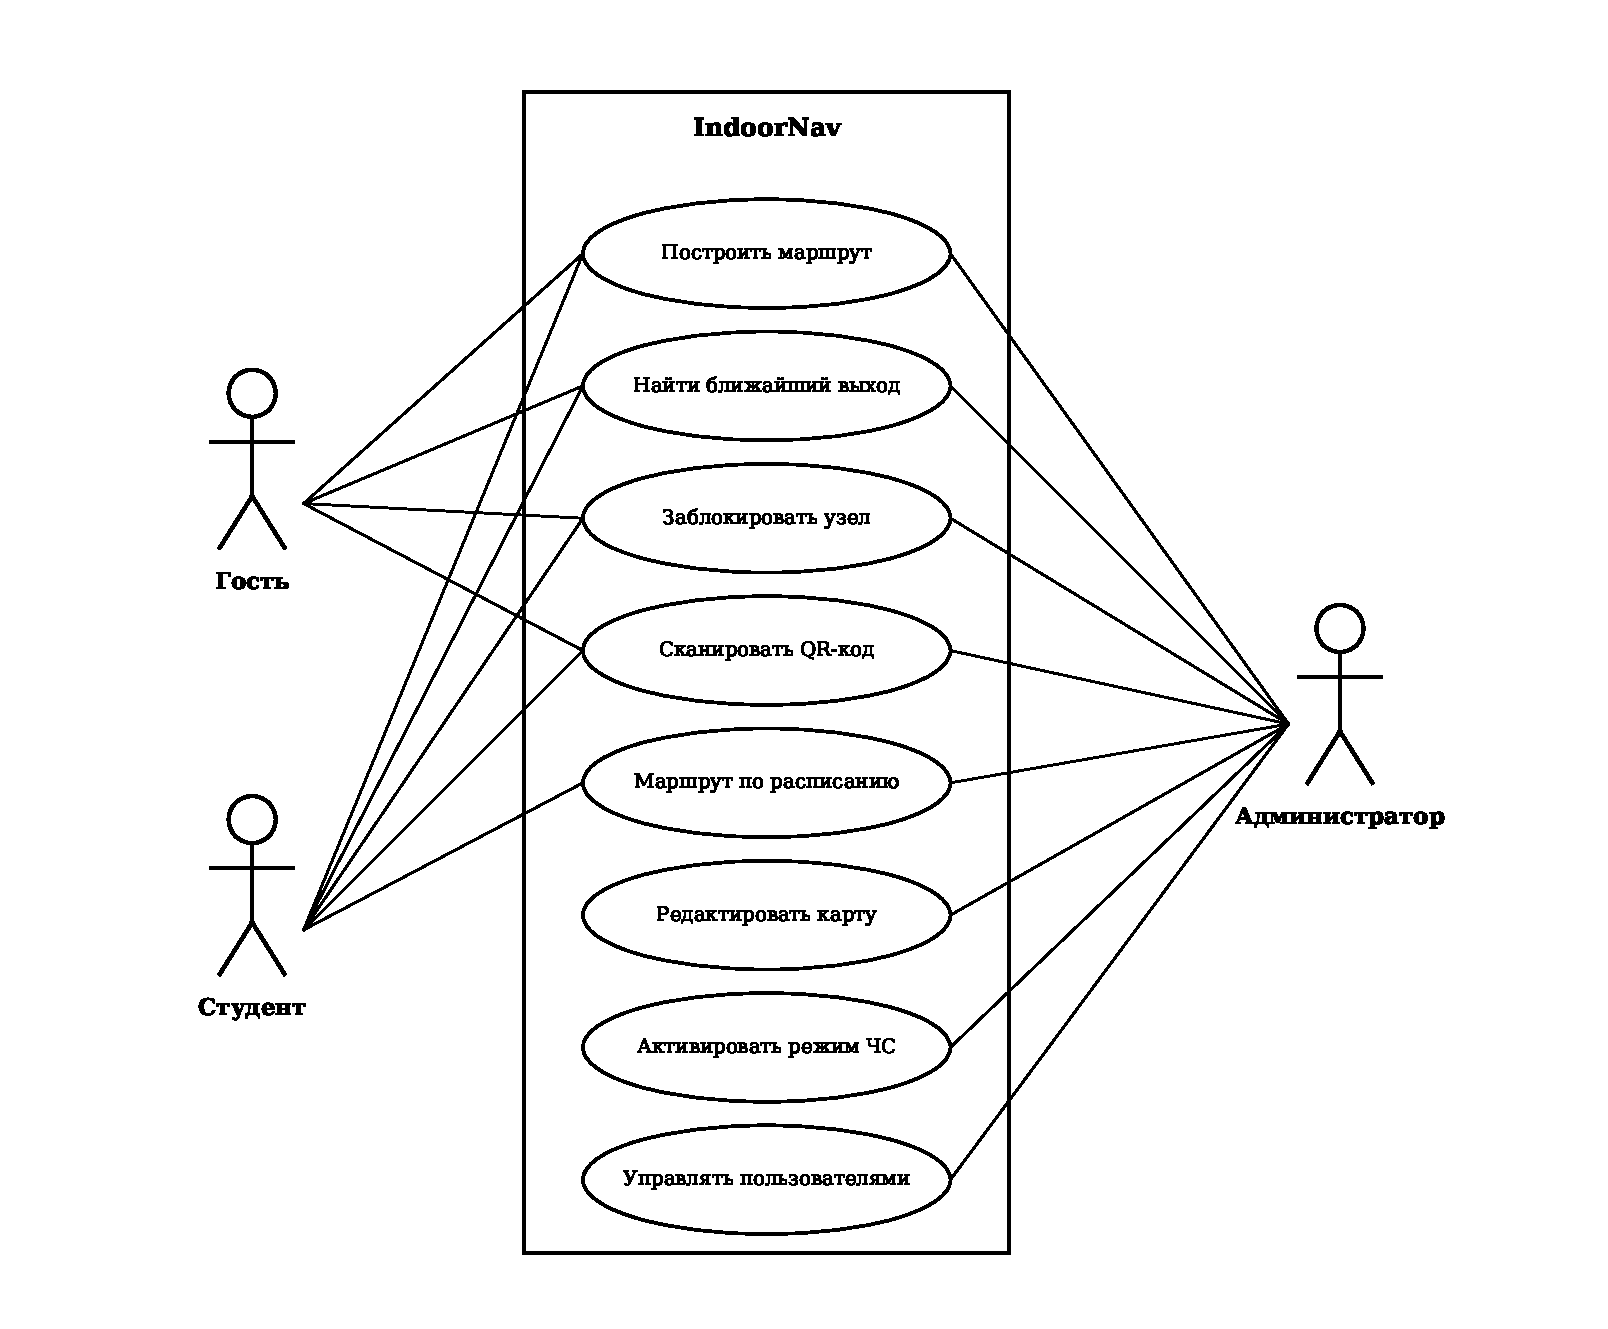
\includegraphics[width=0.95\textwidth]{Pictures/usecase.eps}
	\caption{Диаграмма вариантов использования}
	\label{usecase:image}
\end{figure}

Ниже подробно разобраны три ключевых сценария: построение повседневного маршрута, эвакуация и перестроение маршрута при блокировке.

\subsubsection{Построение маршрута}

Сценарий навигации:
\begin{enumerate}
\item Пользователь выбирает начальную точку (вручную или через QR).
\item Пользователь выбирает конечную точку (поиск по названию или нажатием на карту).
\item ViewModel вызывает метод \texttt{NavGraph.FindPath(startId, endId, excludeIds)}.
\item Алгоритм Дейкстры строит кратчайший путь с учётом исключённых узлов.
\item Маршрут возвращается как упорядоченный список узлов.
\item ViewModel формирует пошаговые инструкции и отображает маршрут на карте.
\end{enumerate}

\subsubsection{Построение эвакуационного маршрута}

Сценарий эвакуации:
\begin{enumerate}
\item Система получает от сервера флаг активации ЧС.
\item ViewModel вызывает метод \texttt{EmergencyService.FindNearestExitRoute(start, graph, blocked)}.
\item Сервис определяет все доступные эвакуационные выходы в текущем здании.
\item Для каждого выхода вычисляется кратчайший путь алгоритмом Дейкстры.
\item Маршрут возвращается как список узлов от текущего положения до выхода.
\item При отсутствии достижимых выходов возвращается пустой список.
\end{enumerate}

\subsubsection{Блокировка участка и перестроение маршрута}

Сценарий обхода препятствия:
\begin{enumerate}
\item Пользователь нажимает на узел и выбирает <<Заблокировать>>.
\item Идентификатор узла добавляется в множество заблокированных (\texttt{HashSet<string>}).
\item ViewModel формирует множество исключений: все выходы (кроме начального и конечного) и заблокированные узлы.
\item Вызывается метод \texttt{FindPath} с обновлённым множеством исключений.
\item Алгоритм строит маршрут в обход заблокированного узла.
\item Если путь отсутствует, то отображается сообщение <<Маршрут не найден>>.
\end{enumerate}

\subsection{Требования к тестированию}

\subsubsection{Объём тестирования}

Разработка должна включать:
\begin{itemize}
\item модульные тесты для алгоритма Дейкстры;
\item модульные тесты для алгоритма поиска ближайшего выхода;
\item тесты производительности (замеры времени выполнения на разных размерах графа);
\item тесты с динамическим исключением узлов (последовательная блокировка пути);
\item тесты на корректность весов рёбер (межэтажные переходы, евклидово расстояние).
\end{itemize}

\subsubsection{Критерии приёмки}

Модуль считается готовым при выполнении (согласно ГОСТ 19.301-79 \cite{gost19301}):
\begin{itemize}
\item успешного прохождения всех модульных и интеграционных тестов;
\item соответствия требованиям производительности (замеры < 200 мс для 500 узлов);
\item корректной работы на тестовых данных реального здания;
\item документирования публичного API (классы \texttt{NavGraph}, \texttt{NavNode}, \texttt{NavEdge}, методы \texttt{FindPath}, \texttt{FindNearestExitRoute});
\item отсутствия утечек памяти при многократных вызовах.
\end{itemize}

\subsection{Требования к программной документации}

Программная документация должна соответствовать ГОСТ 19.105-78 \cite{gost19105} и включать:
\begin{itemize}
\item описание алгоритма Дейкстры и его модификаций для динамического исключения;
\item описание структур данных навигационного графа;
\item описание алгоритма поиска ближайшего эвакуационного выхода;
\item описание механизма учёта межэтажных переходов;
\item результаты тестирования производительности и корректности;
\item рекомендации по оптимизации и дальнейшему развитию.
\end{itemize}

% !TeX root = mainstarkov.tex
% !TeX program = xelatex
% !TeX encoding = UTF-8
\section{Технический проект}

\subsection{Общая характеристика организации решения задачи}

Разрабатываемый модуль динамической маршрутизации является алгоритмическим ядром системы IndoorNav и обеспечивает построение оптимальных маршрутов внутри здания с учётом динамически изменяющихся препятствий. Модуль не зависит от пользовательского интерфейса и может использоваться как в мобильном приложении, так и в серверных компонентах.

Архитектура модуля следует принципу разделения ответственности: структуры данных графа выделены в отдельные классы (\texttt{NavNode}, \texttt{NavEdge}, \texttt{NavGraph}), алгоритмы поиска пути инкапсулированы в методах класса \texttt{NavGraph}, а специфичная логика эвакуации вынесена в сервис \texttt{EmergencyService}. Такое разделение упрощает тестирование: алгоритм Дейкстры можно проверять независимо от логики ЧС, а структуры данных -- независимо от алгоритмов. Разделение ответственности между классами опирается на типовые приёмы объектно-ориентированного проектирования \cite{gof,freeman} и принципы чистой архитектуры \cite{fowler}.

Система построена по архитектурному шаблону MVVM \cite{mauimvvm,albahari} и разделена на четыре слоя: слой представления (View), слой моделей представления (ViewModel), сервисный слой (Service) и слой моделей данных (Model); ниже располагается хранилище данных в формате JSON. Схема архитектуры программной системы с указанием состава компонентов и связей между слоями приведена на рисунке~\ref{arch:image}. Компоненты, реализующие динамическую маршрутизацию (\texttt{MainViewModel}, \texttt{NavGraphService}, \texttt{EmergencyService}, \texttt{NavGraph}, \texttt{NavNode}, \texttt{NavEdge}, \texttt{RouteStep}), выделены на схеме цветом.

\begin{figure}[H]
\centering
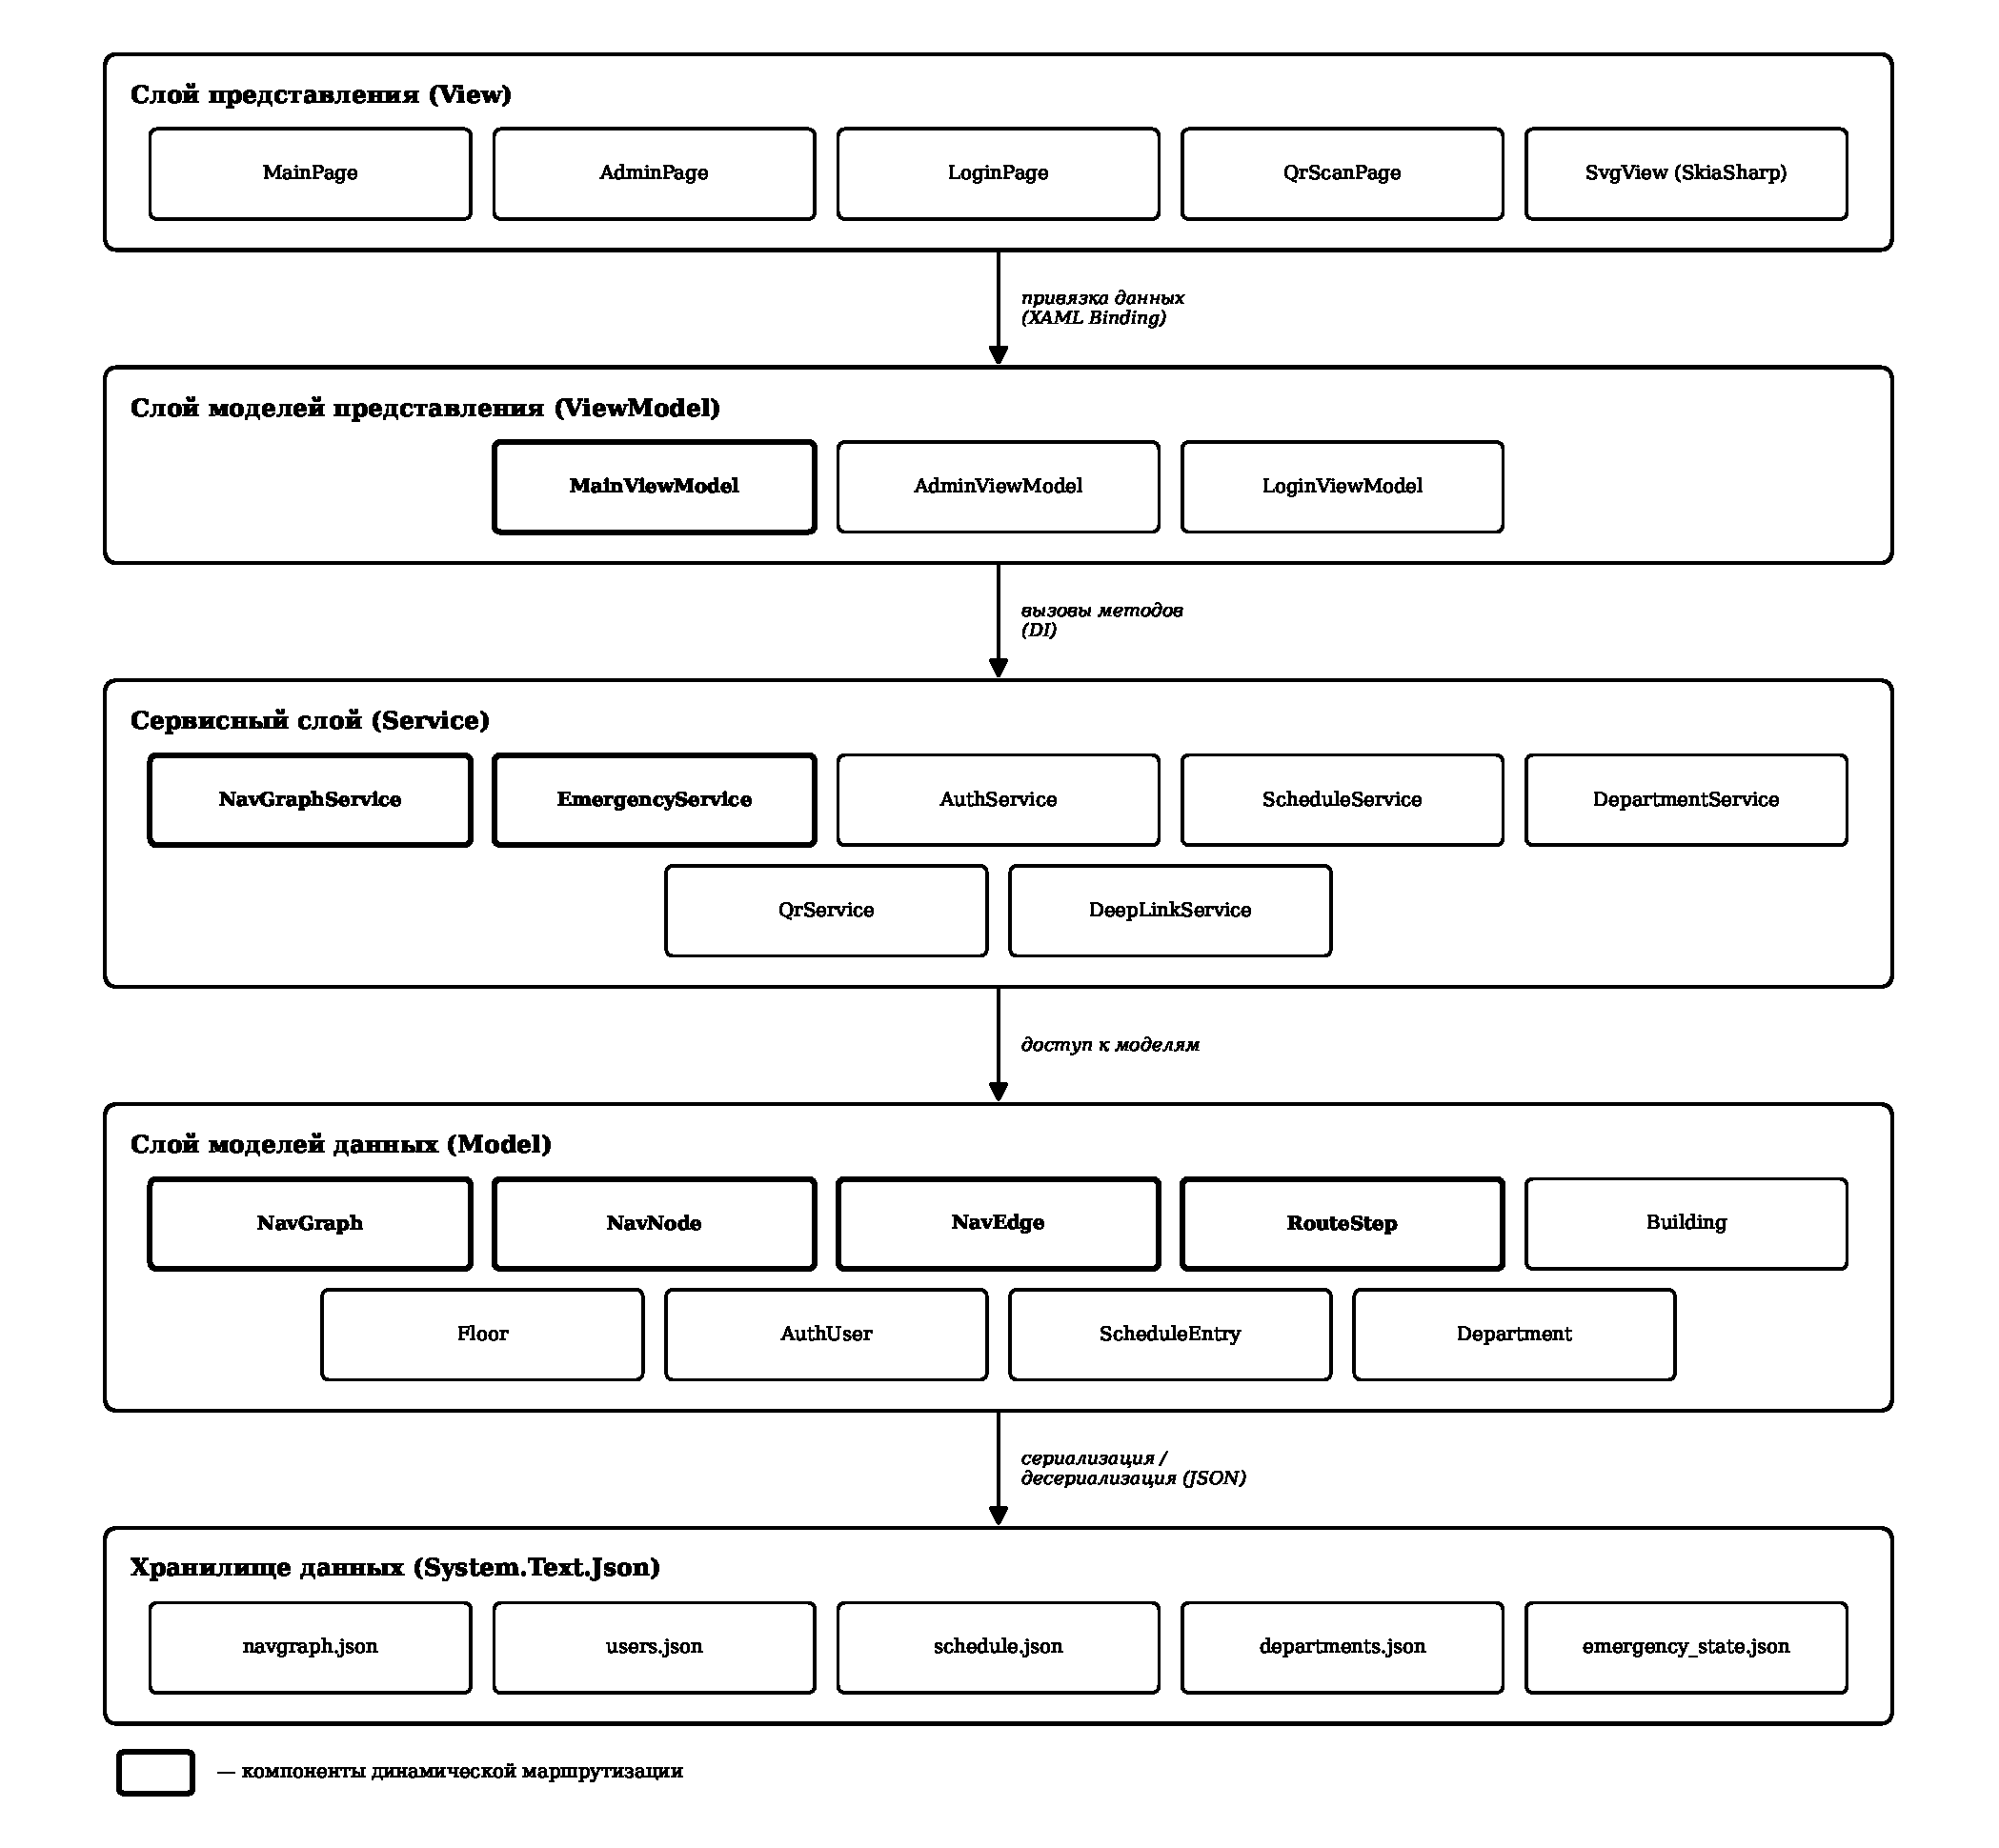
\includegraphics[width=\textwidth]{Pictures/arch.eps}
\caption{Схема архитектуры программной системы IndoorNav}
\label{arch:image}
\end{figure}

Каждый слой зависит только от нижележащего: представление взаимодействует с моделями представления через механизм привязки данных XAML \cite{xaml}, модели представления вызывают методы сервисов через внедрение зависимостей (DI), сервисы оперируют моделями данных, а сохранение и загрузка графа, пользователей, расписания и состояния ЧС выполняются сериализацией моделей в JSON средствами \texttt{System.Text.Json}. Такая слоистая организация изолирует алгоритмическое ядро от пользовательского интерфейса и платформенных особенностей \cite{yarovaya2022,marinin2024}.

Главная особенность решения -- поддержка динамического исключения узлов без модификации исходного графа. Это позволяет системе перестраивать маршруты в реальном времени при блокировке проходов, не перезагружая данные и не создавая копии графа. Исключённые узлы передаются как параметр алгоритма и проверяются при обходе рёбер.

\subsection{Обоснование выбора технологий реализации}

\subsubsection{Язык C\# и платформа .NET.}

Реализация выполнена на языке C\# \cite{richter} в рамках платформы .NET MAUI \cite{maui}, что обеспечивает единый код для Android, iOS и Windows. Кроссплатформенный подход выбран вместо нативной разработки под каждую ОС: он сохраняет единую кодовую базу, что подтверждается опытом перехода от Xamarin к .NET MAUI \cite{ershov2021,ilichev2018} и сравнительными исследованиями кроссплатформенных мобильных технологий \cite{zhukovskaya2017,eskendir2019,feshina2022,jia2018}. C\# предоставляет строгую типизацию для моделирования навигационного графа, обобщённые коллекции (\texttt{Dictionary}, \texttt{SortedSet}, \texttt{HashSet}) для эффективной реализации алгоритмов и LINQ для фильтрации узлов по зданию, этажу и типу.

\subsubsection{Стандартные коллекции .NET.} 

Для реализации алгоритма Дейкстры используются стандартные коллекции .NET без привлечения сторонних библиотек: \texttt{SortedSet<(float, string)>} для очереди с приоритетом, \texttt{Dictionary<string, float>} для расстояний, \texttt{Dictionary<string, string?>} для предшественников, \texttt{HashSet<string>} для исключённых узлов. Это обеспечивает отсутствие внешних зависимостей и простоту отладки.

\subsubsection{Сериализация System.Text.Json.} 

Загрузка и сохранение навигационного графа выполняется с использованием \texttt{System.Text.Json} \cite{systemtextjson} с настройкой \texttt{WriteIndented = true}. Формат JSON \cite{json} выбран как компактный, читаемый и поддерживаемый на всех целевых платформах; среди форматов хранения текстовых данных он даёт хороший баланс между размером и удобством обработки \cite{naumov2021}.

\subsection{Архитектура алгоритмического ядра}

Модуль маршрутизации состоит из следующих компонентов:
\begin{itemize}
\item \textbf{NavNode} -- класс узла графа с атрибутами (координаты, этаж, тип, флаги);
\item \textbf{NavEdge} -- класс ребра графа (связь между узлами с весом);
\item \textbf{NavGraph} -- класс графа, хранящий узлы и рёбра, предоставляющий методы поиска пути;
\item \textbf{EmergencyService} -- сервис поиска ближайшего эвакуационного выхода;
\item \textbf{NavGraphService} -- сервис загрузки, сохранения и предоставления графа.
\end{itemize}

Все компоненты регистрируются в контейнере внедрения зависимостей (\texttt{MauiProgram.cs}) как singleton \cite{mauidi}, что обеспечивает единый экземпляр на всё время работы приложения и согласованность состояния. Внедрение зависимостей снижает связанность модулей и упрощает их раздельное тестирование \cite{sazonov2024,uvarov2016}.

Схема взаимодействия слоёв MVVM с выделением алгоритмического модуля приведена на рисунке~\ref{starkovmvvm:image}.

\begin{figure}[H]
\centering
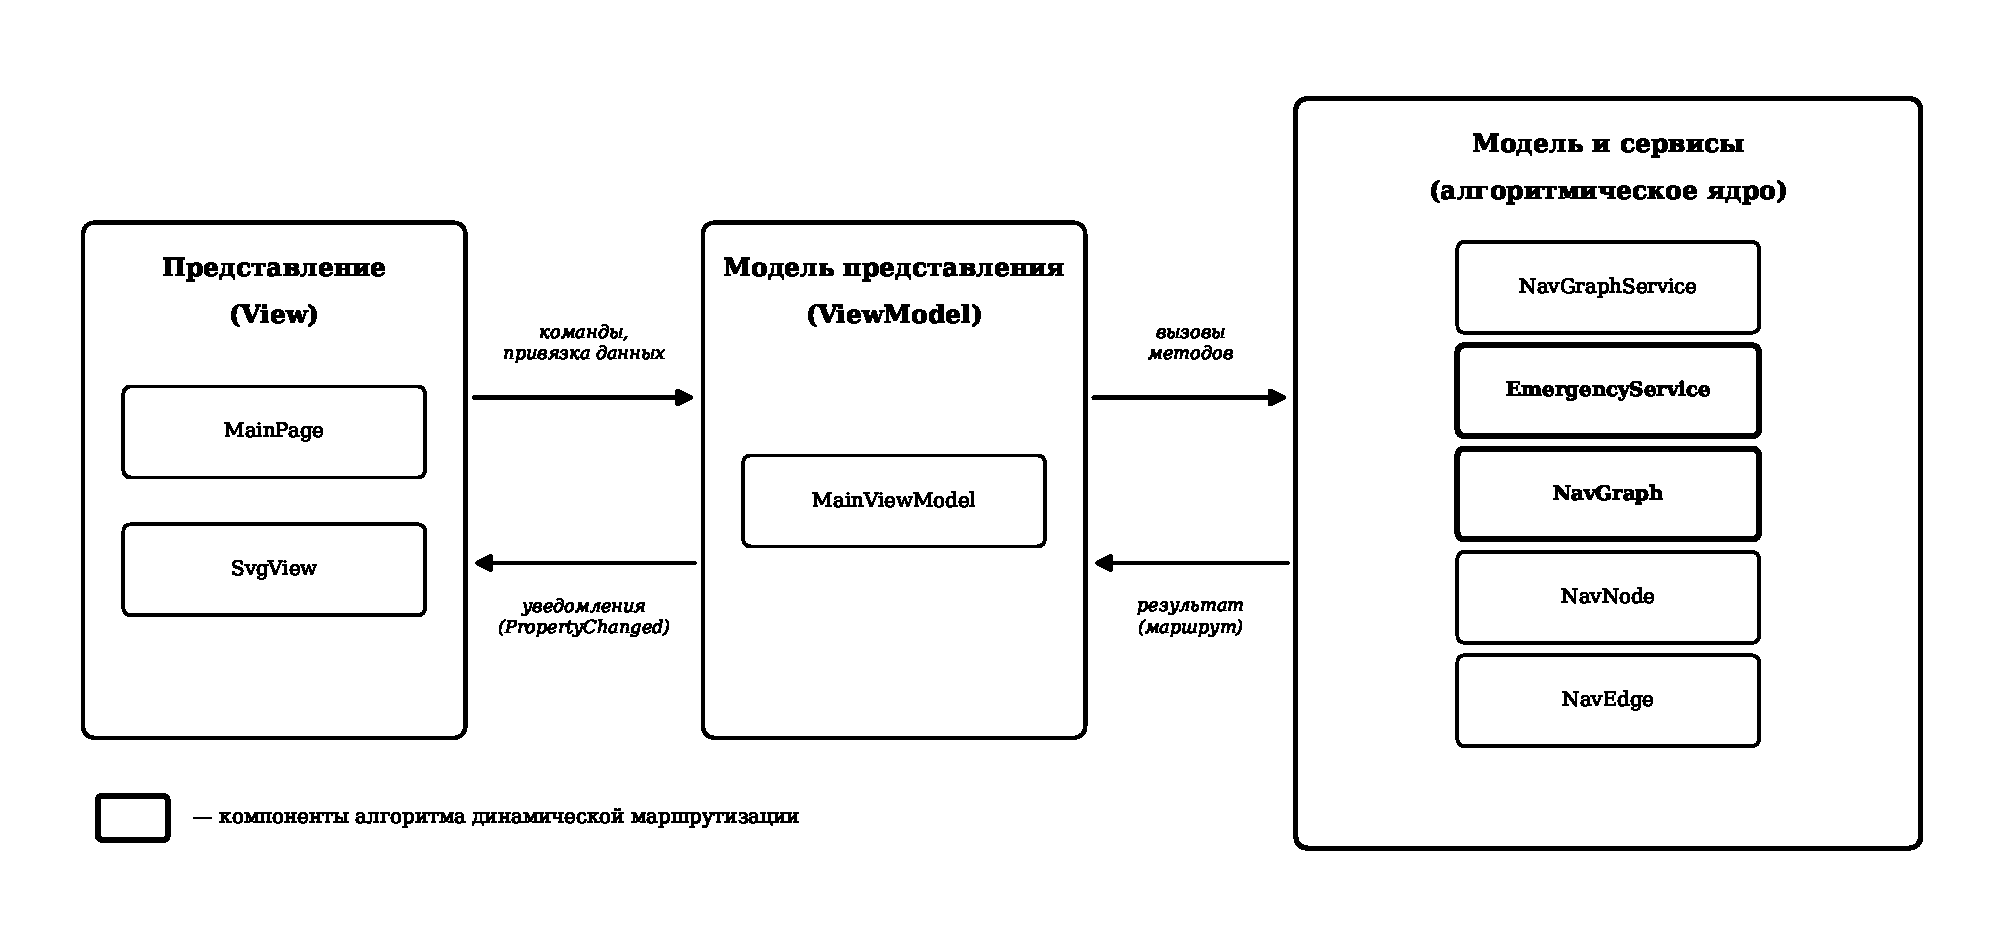
\includegraphics[width=0.95\textwidth]{Pictures/starkovmvvm.eps}
\caption{MVVM-архитектура приложения с выделением алгоритмического модуля}
\label{starkovmvvm:image}
\end{figure}

\subsection{Структуры данных навигационного графа}

\subsubsection{Класс NavNode.} 

Узел графа представляет точку на плане этажа (помещение, коридор, перекрёсток, лестничная площадка, выход) и содержит следующие свойства:
\begin{itemize}
\item \texttt{Id} -- уникальный идентификатор узла (string);
\item \texttt{Name} -- отображаемое название для пользователя (string);
\item \texttt{X}, \texttt{Y} -- координаты на плане этажа в условных единицах (float);
\item \texttt{FloorNumber} -- номер этажа (int), используется для определения межэтажных переходов;
\item \texttt{BuildingId} -- идентификатор здания/корпуса (string);
\item \texttt{IsTransition} -- флаг узла перехода между этажами;
\item \texttt{IsElevator} -- флаг лифтового узла;
\item \texttt{IsExit} -- флаг основного выхода;
\item \texttt{IsEvacuationExit} -- флаг эвакуационного выхода;
\item \texttt{IsFireExtinguisher} -- флаг огнетушителя (отображается при ЧС);
\item \texttt{IsQrAnchor} -- флаг QR-якоря для позиционирования;
\item \texttt{IsRoom} -- флаг узла-аудитории;
\item \texttt{IsWaypoint} -- флаг путевой точки;
\item \texttt{IsHidden} -- флаг скрытого узла (не отображается на карте);
\item \texttt{TransitionGroupId} -- идентификатор группы перехода для связывания узлов на разных этажах;
\item \texttt{RoomId} -- необязательный идентификатор помещения из внешней системы.
\end{itemize}

Узлы с флагами \texttt{IsExit} и \texttt{IsEvacuationExit} используются как целевые точки при построении эвакуационного маршрута.

\subsubsection{Класс NavEdge.} 

Ребро графа представляет проход между двумя точками и содержит:
\begin{itemize}
\item \texttt{FromId}, \texttt{ToId} -- идентификаторы соединяемых узлов;
\item \texttt{Weight} -- вес ребра, вычисляемый как расстояние между узлами с учётом типа прохода;
\item \texttt{IsCrossFloor} -- флаг межэтажного перехода.
\end{itemize}

Вес ребра вычисляется автоматически при создании: для узлов на одном этаже $w = \sqrt{(x_2 - x_1)^2 + (y_2 - y_1)^2}$, для узлов на разных этажах $w = 150$.

Фиксированный штраф 150 для межэтажных переходов отражает повышенные затраты времени на подъём/спуск по лестнице или лифту. Граф является неориентированным: при добавлении ребра создаются две направленные записи (от A к B и от B к A) с одинаковым весом.

\subsubsection{Класс NavGraph.} 

Граф хранит коллекции узлов и рёбер и предоставляет алгоритмы поиска пути:

\begin{itemize}
\item \texttt{Nodes} -- список всех узлов графа (\texttt{List<NavNode>});
\item \texttt{Edges} -- список всех рёбер графа (\texttt{List<NavEdge>});
\item \texttt{GetNode(id)} -- быстрый доступ к узлу по идентификатору через внутренний словарь;
\item \texttt{FindPath(startId, endId, excludeIds)} -- поиск кратчайшего пути методом Дейкстры;
\item \texttt{BuildAdjacency()} -- построение списка смежности для оптимизации поиска.
\end{itemize}

Метод \texttt{BuildAdjacency()} строит словарь связей \texttt{Dictionary<string, List<(string neighbor, float weight)>>}, который используется алгоритмом Дейкстры для быстрого доступа к соседям каждой вершины. Построение выполняется один раз при загрузке графа.

Пример навигационного графа здания приведён на рисунке~\ref{navgraph:image}. Узлы обозначены кружками с идентификаторами, рёбра -- линиями с указанием веса. Узлы-выходы выделены двойной рамкой, узлы переходов между этажами -- штриховой рамкой.

\begin{figure}[H]
\centering
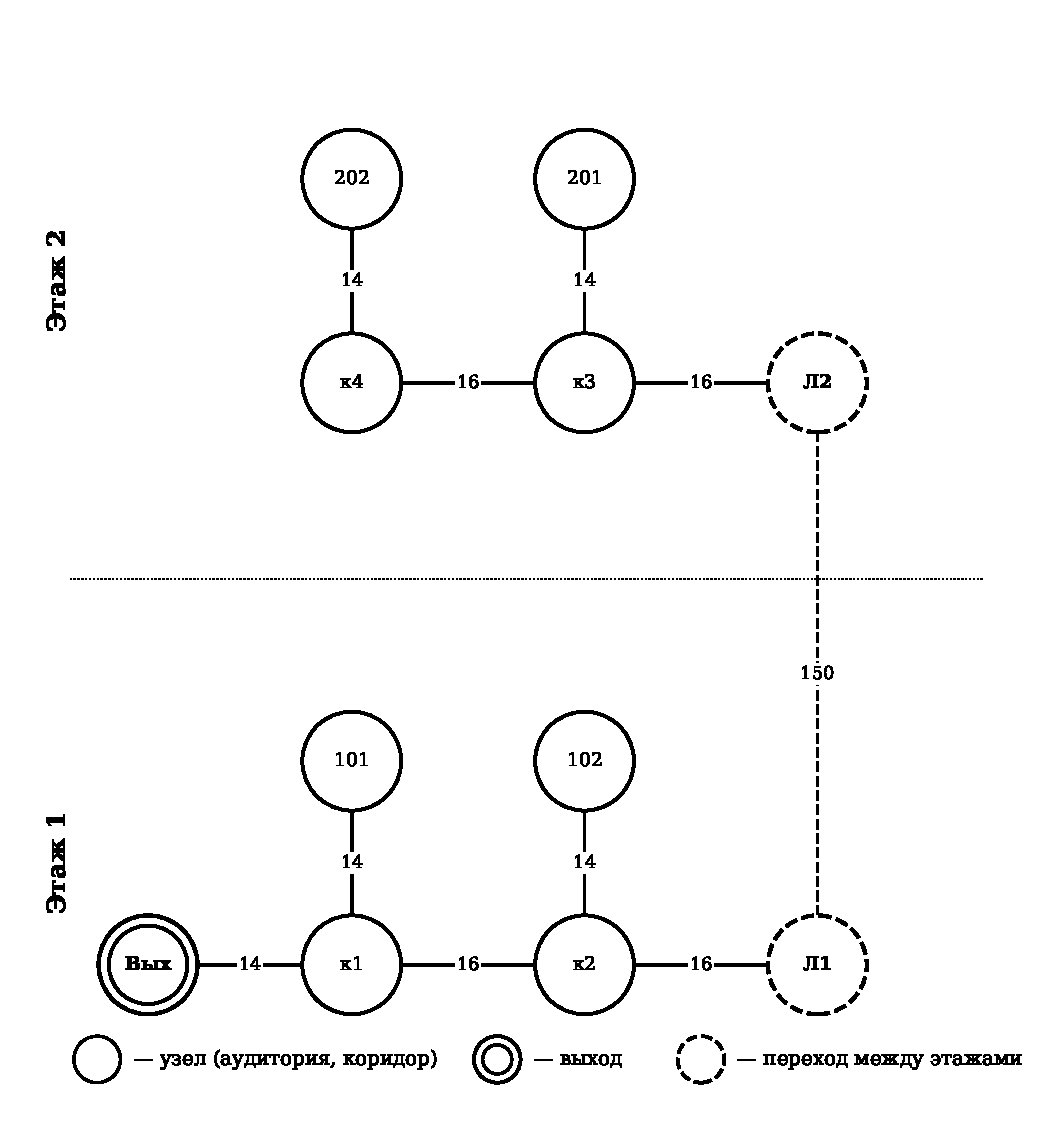
\includegraphics[width=0.85\textwidth]{Pictures/graf.eps}
\caption{Пример структуры навигационного графа здания}
\label{navgraph:image}
\end{figure}

\subsection{Проектирование хранения данных}

Все данные приложения хранятся локально, в текстовых файлах формата JSON~-- так навигация не зависит от сети, а файлы при необходимости легко просмотреть и поправить вручную. Чтение и запись идут через \texttt{System.Text.Json}: объекты модели преобразуются в формат JSON и обратно без использования промежуточного слоя базы данных \cite{vinnikov2022}. Данный подход оправдан для навигационного графа здания, поскольку граф полностью размещается в оперативной памяти, а его модификация происходит редко — преимущественно при разметке карты администратором.

Перечень файлов данных и их назначение приведены в таблице~\ref{datafiles:table}.

\begin{xltabular}{\textwidth}{|l|X|}
	\caption{Файлы данных приложения\label{datafiles:table}}\\ \hline
	\centrow Файл & \centrow Содержимое \\ \hline
	\thead{1} & \centrow 2 \\ \hline
	\endfirsthead
	\continuecaption{Продолжение таблицы \ref{datafiles:table}}
	\centrow Файл & \centrow Содержимое \\ \hline
	\finishhead
	\texttt{navgraph.json} & Навигационный граф: массивы узлов и рёбер \\ \hline
	\texttt{users.json} & Учётные записи с хешами паролей и ролями \\ \hline
	\texttt{departments.json} & Кафедры и учебные группы \\ \hline
	\texttt{schedule.json} & Расписание занятий по аудиториям и группам \\ \hline
	\texttt{emergency\_state.json} & Список зданий, где включён режим ЧС
\end{xltabular}

Главный для маршрутизации файл~-- \texttt{navgraph.json}. На верхнем уровне это объект с двумя массивами: \texttt{Nodes} (узлы) и \texttt{Edges} (рёбра). Каждый узел хранит идентификатор, координаты, этаж, корпус и набор флагов типа; каждое ребро~-- идентификаторы концов, длина и признак межэтажного перехода. Структура напрямую повторяет классы \texttt{NavNode} и \texttt{NavEdge}, поэтому отдельная схема преобразования не нужна. Фрагмент файла с одним узлом и одним ребром выглядит так:

\newpage
\begin{figure}[H] 
\begin{lstlisting}
{
	"Nodes": [
	{ "Id": "a-101", "Name": "101", "X": 320.5, "Y": 148.0,
		"FloorNumber": 1, "BuildingId": "A",
		"IsRoom": true, "IsExit": false, "IsEvacuationExit": false }
	],
	"Edges": [
	{ "FromId": "a-101", "ToId": "a-kor1", "Weight": 42.3,
		"IsCrossFloor": false }
	]
}
\end{lstlisting}
\end{figure}

При запуске \texttt{NavGraphService} читает файл в объект \texttt{NavGraph}, после чего граф готов к работе. Сохранение выполняется обратной операцией с отступами (\texttt{WriteIndented}), чтобы файл оставался читаемым.

\subsection{Проектирование алгоритмов маршрутизации}

Алгоритмы маршрутизации включают четыре компонента: построение кратчайшего маршрута по алгоритму Дейкстры, поиск ближайшего эвакуационного выхода, формирование пошаговых инструкций и определение множества заблокированных узлов.

\subsubsection{Реализация алгоритма Дейкстры}

Реализация алгоритма Дейкстры в методе \texttt{NavGraph.FindPath(startId, endId, excludeIds)} использует следующие структуры данных:
\begin{itemize}
\item \texttt{SortedSet<(float dist, string id)>} -- очередь с приоритетом для выбора вершины с минимальным расстоянием;
\item \texttt{Dictionary<string, float>} -- словарь текущих кратчайших расстояний от стартовой вершины;
\item \texttt{Dictionary<string, string?>} -- словарь предшественников для восстановления пути;
\item \texttt{ISet<string>?} -- множество исключаемых узлов (может быть null).
\end{itemize}.

\textbf{Динамическое исключение узлов.} Множество исключаемых узлов передаётся как параметр \texttt{excludeIds} и проверяется при рассмотрении соседей. Это позволяет исключать узлы без модификации графа. Конечный узел маршрута никогда не исключается, даже если его идентификатор присутствует в множестве.

\textbf{Обработка отсутствия пути.} Если после завершения алгоритма расстояние до целевой вершины остаётся равным \texttt{float.MaxValue} (вершина недостижима), метод возвращает пустой список. Это обеспечивает устойчивость системы: при полной блокировке пути приложение корректно информирует пользователя.

\textbf{Оптимизация списка смежности.} Перед запуском алгоритма строится словарь смежности \texttt{adj}, группирующий рёбра по исходящему узлу. Это позволяет получить всех соседей вершины за $O(1)$ вместо линейного поиска по списку рёбер.

\textbf{Обработка устаревших записей очереди.} При обновлении расстояния до вершины старая запись не удаляется из \texttt{SortedSet}, а проверяется при извлечении: если извлечённое расстояние превышает текущее, запись игнорируется. Это упрощает реализацию и избавляет от необходимости сложного обновления приоритетов.

\subsubsection{Алгоритм поиска ближайшего эвакуационного выхода}

Для режима чрезвычайной ситуации реализован алгоритм в методе \texttt{EmergencyService.FindNearestExitRoute(start, graph, excludeIds)}, который находит кратчайший путь до ближайшего эвакуационного выхода. Пример: 

\begin{figure}[H] 
\begin{lstlisting}
function FindNearestExitRoute(start, graph, excludeIds):

  exits = graph.Nodes.Where(n =>
    (n.IsExit or n.IsEvacuationExit)
    and n.BuildingId == start.BuildingId
    and excludeIds not contains n.Id)

  if exits is empty:
    exits = graph.Nodes.Where(n =>
      (n.IsExit or n.IsEvacuationExit)
      and excludeIds not contains n.Id)
  if exits is empty:
    return []

  dist[start.Id] = 0
  for each node in graph.Nodes:
    if node.Id != start.Id:
      dist[node.Id] = +infinity
    prev[node.Id] = null
  queue.Add((0, start.Id))
  adj = BuildAdjacency(graph)

  while queue is not empty:
    (d, uid) = queue.ExtractMin()
    if d > dist[uid]: continue
    for each (nid, w) in adj[uid]:
      if nid != start.Id and excludeIds contains nid:
        continue
      alt = d + w
      if alt < dist[nid]:
        queue.Remove((dist[nid], nid))
        dist[nid] = alt
        prev[nid] = uid
        queue.Add((alt, nid))

  bestExit = exits.OrderBy(e => dist[e.Id]).First()
  if bestExit == null or dist[bestExit.Id] == +infinity:
    return []

  path = []
  current = bestExit.Id
  while current != null:
    path.Add(nodeMap[current])
    current = prev[current]
  path.Reverse()
  return path
\end{lstlisting}
\end{figure}

\textbf{Интеграция с ViewModel.} При активации режима ЧС \texttt{MainViewModel} вызывает \texttt{ExecuteBuildEmergencyRoute()}, который определяет текущее положение пользователя (\texttt{StartNode}), формирует множество заблокированных узлов (\texttt{\_blockedNodeIds}), вызывает \texttt{EmergencyService.FindNearestExitRoute(start, graph, blocked)}, при наличии пути устанавливает конечный узел и вызывает \texttt{ExecuteBuildRoute()}, при отсутствии пути отображает сообщение <<Маршрут до выхода не найден>>.

\subsubsection{Механизм формирования пошаговых инструкций}

После построения маршрута \texttt{MainViewModel.BuildRouteSteps(path)} формирует пошаговые текстовые инструкции для пользователя. Метод группирует узлы маршрута по этажам в сегменты: для каждого сегмента определяется направление движения и формируется текст инструкции. Для межэтажных переходов добавляется шаг <<Перейдите на этаж N>> с указанием типа перехода (лестница/лифт). Каждому шагу назначается иконка (прямо, поворот, лестница, лифт, выход), определяется фокусный узел и прямоугольник для подсветки на карте. После формирования обновляются свойства интерфейса: \texttt{RouteSteps}, \texttt{CurrentStep}, \texttt{HasRoute}.

\subsubsection{Множество исключённых узлов}

Метод \texttt{MainViewModel.BuildExcludeSet(start, end)} формирует множество узлов, исключаемых из маршрута. В множество включаются все узлы с флагом \texttt{IsExit} или \texttt{IsEvacuationExit}, кроме стартового и конечного, а также все узлы, заблокированные пользователем (\texttt{\_blockedNodeIds}). Исключение выходов, не являющихся целевыми, предотвращает прохождение маршрута через другие выходы, что особенно важно в режиме эвакуации. Заблокированные узлы добавляются к множеству исключений, обеспечивая автоматическое перестроение маршрута в обход непроходимых участков.

\subsection{Процесс построения маршрута}

Описанные алгоритмы и структуры данных связываются в единый поток обработки запроса. Путь от действия пользователя до маршрута на экране проходит через все слои приложения и показан на рисунке~\ref{routeflow:image}.

\begin{figure}[H]
	\centering
	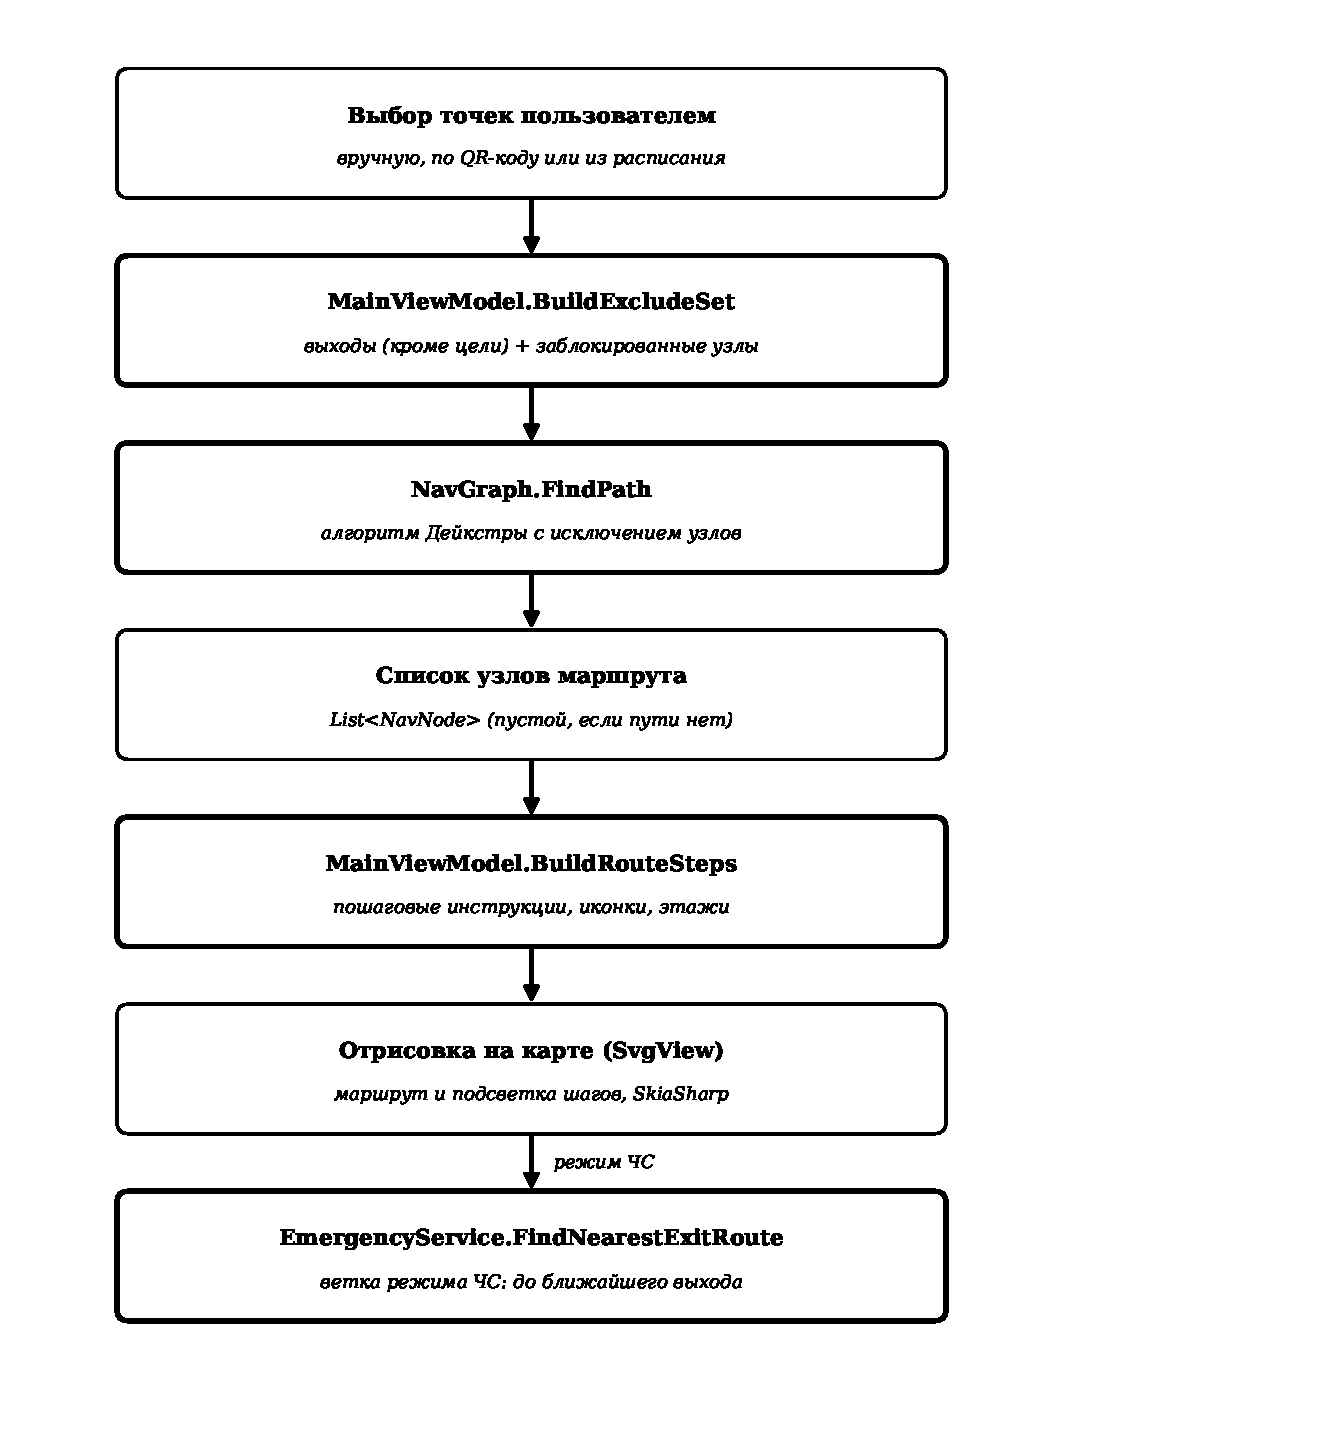
\includegraphics[width=0.7\textwidth]{Pictures/routeflow.eps}
	\caption{Процесс построения маршрута по слоям приложения}
	\label{routeflow:image}
\end{figure}

Сначала пользователь задаёт начальную и конечную точки~-- вручную, сканированием QR-кода или выбором аудитории из расписания. Затем \texttt{MainViewModel} собирает множество исключаемых узлов (\texttt{BuildExcludeSet}) и передаёт его вместе с концами маршрута в \texttt{NavGraph.FindPath}. Алгоритм Дейкстры возвращает список узлов; если он пуст, пользователю выводится сообщение о недоступности пути. Непустой маршрут уходит в \texttt{BuildRouteSteps}, который превращает его в пошаговые инструкции, после чего \texttt{SvgView} отрисовывает путь и подсвечивает текущий шаг на плане этажа.

В режиме ЧС поток выполнения отличается: вместо обычного построения маршрута вызывается \texttt{EmergencyService.FindNearestExitRoute}, который самостоятельно определяет ближайший выход, после чего обработка продолжается по той же цепочке (список узлов, инструкции, отрисовка). Единый поток выполнения позволяет обоим сценариям, повседневному и эвакуационному, использовать один и тот же код отображения.

\subsection{Проектирование пользовательского интерфейса}

Интерфейс проектировался по принципам человеко-ориентированного проектирования и удобства пользователя \cite{urbanovich2023,sterlyagov2017}: меньше действий до результата (маршрут строится не более чем в три касания), понятные подписи и адаптивная вёрстка под телефон и настольный компьютер. Разметка экранов описана на XAML, а данные связаны с моделями представления через привязку, поэтому одна и та же логика работает на всех платформах.

Приложение состоит из нескольких экранов:
\begin{enumerate}
	\item \textbf{Экран входа.} Гость заходит одним нажатием, студент~-- по логину и паролю. Роль определяет доступные дальше возможности.
	\item \textbf{Главный экран.} Занимает большую часть~-- интерактивный план этажа (контрол \texttt{SvgView} на SkiaSharp \cite{skiasharp}) с панорамированием и масштабированием. Сверху~-- поля <<Откуда>> и <<Куда>> с поиском по списку узлов и автодополнением по названию и тегам, кнопка построения маршрута и переключатель здания и этажа. После построения снизу появляются карточки пошаговых инструкций с кнопками <<Далее>>/<<Назад>> и счётчиком шагов; при ЧС сверху выводится предупреждающий баннер.
	\item \textbf{Экран QR-сканера.} Камера для считывания кода со стены (на Android и iOS); распознанный код задаёт начальную точку.
	\item \textbf{Панель администратора.} Редактор карты (добавление и соединение узлов, выбор их типа), управление пользователями и расписанием, включение режима ЧС по корпусам.
\end{enumerate}

Маршрут на плане выделяется отдельной линией с подсветкой текущего шага, а узлы-выходы и переходы между этажами обозначаются разными значками~-- чтобы пользователь различал их без подписей. Внешний вид главного экрана с построенным маршрутом приведён в разделе системного тестирования (рисунок~\ref{rproute:image}).

\subsection{Тестирование алгоритмов}

\textbf{Модульные тесты.} Разработан набор модульных тестов, покрывающих следующие сценарии: построение простого маршрута (линейный граф из 3 узлов), выбор оптимального пути при наличии альтернатив (разветвлённый граф), корректная работа на графе с циклами, обработка несуществующих идентификаторов узлов (возврат пустого списка), построение маршрута при исключении одного узла, полная блокировка пути (исключение всех промежуточных узлов, возврат пустого результата), поиск ближайшего выхода из нескольких вариантов, работа с одноузловым графом (старт = конец, возврат списка из одного элемента), маршрут с межэтажным переходом (проверка штрафного веса 150), последовательное исключение нескольких узлов, исключение конечного узла (должен быть достижим независимо от множества), пустой граф (нет узлов, возврат пустого списка), несвязный граф (старт и цель в разных компонентах связности).

\textbf{Тесты производительности.} Проведены замеры времени выполнения на тестовых данных различного объёма: граф с 50 узлами и 80 рёбрами -- среднее время 0,021 мс, граф с 200 узлами и 350 рёбрами -- 0,098 мс, граф с 500 узлами и 900 рёбрами -- 0,297 мс, поиск ближайшего выхода на графе 500 узлов -- 0,630 мс. Все замеры укладываются в требование $<200$ мс для построения маршрута и $<300$ мс для поиска выхода с многократным запасом. Результаты показывают линейный рост времени выполнения с увеличением размера графа, что согласуется с теоретической сложностью $O((V + E) \log V)$ для разреженных графов. Подробные результаты и график зависимости приведены в рабочем проекте (таблица~\ref{rpperf:table}).

\textbf{Интеграционные тесты.} Проведено тестирование с реальными данными навигационного графа здания университета: загрузка графа из \texttt{navgraph.json} и корректная десериализация, построение маршрутов между реальными аудиториями, корректность весов рёбер (совпадение с визуальным расстоянием на плане), поиск эвакуационного маршрута из различных стартовых точек, перестроение маршрута при блокировке реальных проходов.

\subsection{Сопоставление требований и компонентов}

Сопоставление требований, сформулированных в техническом задании, и компонентов их реализации приведено в таблице~\ref{algreq:table}.

\begin{xltabular}{\textwidth}{|X|X|}
\caption{Сопоставление требований и компонентов реализации\label{algreq:table}}\\ \hline
\centrow Требование & \centrow Компонент реализации \\ \hline
\endfirsthead
\continuecaption{Продолжение таблицы \ref{algreq:table}}
\centrow Требование & \centrow Компонент реализации \\ \hline
\finishhead
Поиск кратчайшего пути & \texttt{NavGraph.FindPath()} (алгоритм Дейкстры) \\ \hline
Динамическое исключение узлов & Параметр \texttt{excludeIds} в \texttt{FindPath} \\ \hline
Поиск ближайшего выхода & \texttt{EmergencyService.FindNearestExitRoute()} \\ \hline
Межэтажные переходы & Штрафной вес 150, флаг \texttt{IsCrossFloor} \\ \hline
Восстановление пути & Словарь \texttt{prev} + обратный обход \\ \hline
Структуры данных графа & \texttt{NavNode}, \texttt{NavEdge}, \texttt{NavGraph} \\ \hline
Сериализация & \texttt{System.Text.Json}, формат JSON \\ \hline
Пошаговые инструкции & \texttt{MainViewModel.BuildRouteSteps()} \\ \hline
Множество исключений & \texttt{MainViewModel.BuildExcludeSet()} \\ \hline
Производительность & \texttt{SortedSet}, \texttt{Dictionary}, список смежности
\end{xltabular}

\subsection{Выводы по о техническому проект}

В техническом проекте описана реализация алгоритмического ядра системы IndoorNav: выбор технологий (C\#, .NET, стандартные коллекции), структура модулей (NavNode, NavEdge, NavGraph, EmergencyService, NavGraphService), реализация алгоритма Дейкстры с поддержкой динамического исключения узлов, алгоритм поиска ближайшего эвакуационного выхода, механизм формирования пошаговых инструкций, формирование множества исключённых узлов, результаты модульного тестирования и замеров производительности, сериализация графа в JSON.

Разработанное алгоритмическое ядро обеспечивает эффективное построение эвакуационных маршрутов с учётом динамических препятствий. Использование алгоритма Дейкстры с современными структурами данных гарантирует производительность, соответствующую требованиям реального времени.

\ifПрактика{
   % !TeX root = mainstarkov.tex
% !TeX program = xelatex
% !TeX encoding = UTF-8
\section{Рабочий проект}

\subsection{Общая характеристика рабочего проекта}

Если в техническом проекте приведены проектные решения и псевдокод алгоритмов динамической маршрутизации, то в рабочем проекте представлена их программная реализация на языке C\# в составе приложения IndoorNav и результаты комплексного тестирования. Реализация выполнена в соответствии с проектными решениями технического проекта (таблица~\ref{algreq:table}) и сохраняет принцип разделения ответственности: структуры данных, алгоритмы поиска пути и логика эвакуации реализованы как независимые модули, что обеспечивает возможность их раздельного тестирования.

В процессе разработки алгоритмического ядра динамической маршрутизации выделены следующие программные модули: \texttt{NavNode}, \texttt{NavEdge}, \texttt{NavGraph}, \texttt{NavGraphService}, \texttt{EmergencyService} и \texttt{MainViewModel}. Их состав и распределение по слоям архитектуры приведены в таблице~\ref{rpfiles:table}.

\begin{xltabular}{\textwidth}{|l|c|X|}
\caption{Состав программных модулей алгоритмического ядра\label{rpfiles:table}}\\ \hline
\centrow Модуль (файл) & \centrow Слой & \centrow Назначение \\ \hline
\thead{1} & \thead{2} & \centrow 3 \\ \hline
\endfirsthead
\continuecaption{Продолжение таблицы \ref{rpfiles:table}}
\centrow Модуль (файл) & \centrow Слой & \centrow Назначение \\ \hline
\finishhead
\texttt{NavNode.cs} & Model & Класс узла навигационного графа \\ \hline
\texttt{NavEdge.cs} & Model & Класс ребра графа с весом \\ \hline
\texttt{NavGraph.cs} & Model & Граф и алгоритм Дейкстры (\texttt{FindPath}) \\ \hline
\texttt{NavGraphService.cs} & Service & Загрузка, сохранение и предоставление графа \\ \hline
\texttt{EmergencyService.cs} & Service & Поиск ближайшего эвакуационного выхода \\ \hline
\texttt{MainViewModel.cs} & ViewModel & Построение маршрута, множество исключений, пошаговые инструкции
\end{xltabular}

Далее каждый модуль рассмотрен отдельно: приведены его назначение и таблица реализованных полей или методов с описанием параметров.

\subsection{Модули данных NavNode и NavEdge}

\texttt{NavNode} -- класс узла навигационного графа, представляющий точку на плане этажа (помещение, коридор, перекрёсток, лестничную площадку или выход). \texttt{NavEdge} -- класс ребра графа, представляющий проход между двумя узлами с весом. Это модули данных без вычислительной логики; их ключевые поля приведены в таблицах~\ref{rpnode:table} и~\ref{rpedge:table}.

\begin{xltabular}{\textwidth}{|l|l|X|}
\caption{Ключевые поля класса NavNode\label{rpnode:table}}\\ \hline
\centrow Поле & \centrow Тип & \centrow Описание \\ \hline
\thead{1} & \thead{2} & \centrow 3 \\ \hline
\endfirsthead
\continuecaption{Продолжение таблицы \ref{rpnode:table}}
\centrow Поле & \centrow Тип & \centrow Описание \\ \hline
\finishhead
\texttt{Id} & string & Уникальный идентификатор узла \\ \hline
\texttt{X}, \texttt{Y} & float & Координаты узла на плане этажа \\ \hline
\texttt{FloorNumber} & int & Номер этажа \\ \hline
\texttt{BuildingId} & string & Идентификатор здания (корпуса) \\ \hline
\texttt{IsTransition} & bool & Узел межэтажного перехода (лестница, лифт) \\ \hline
\texttt{IsExit} & bool & Основной выход из здания \\ \hline
\texttt{IsEvacuationExit} & bool & Эвакуационный выход \\ \hline
\texttt{TransitionGroupId} & string & Группа перехода для связывания узлов разных этажей
\end{xltabular}

\begin{xltabular}{\textwidth}{|l|l|X|}
\caption{Поля класса NavEdge\label{rpedge:table}}\\ \hline
\centrow Поле & \centrow Тип & \centrow Описание \\ \hline
\endfirsthead
\continuecaption{Продолжение таблицы \ref{rpedge:table}}
\centrow Поле & \centrow Тип & \centrow Описание \\ \hline
\finishhead
\texttt{FromId}, \texttt{ToId} & string & Идентификаторы соединяемых узлов \\ \hline
\texttt{Weight} & float & Вес ребра (евклидово расстояние или штраф 150) \\ \hline
\texttt{IsCrossFloor} & bool & Признак межэтажного ребра
\end{xltabular}

\subsection{Модуль NavGraph}

\texttt{NavGraph} -- центральный модуль алгоритмического ядра: хранит коллекции узлов и рёбер и реализует поиск кратчайшего пути по алгоритму Дейкстры с поддержкой динамического исключения узлов. Описание реализованных методов приведено в таблице~\ref{rpgraph:table}.

\begin{xltabular}{\textwidth}{|X|X|X|}
\caption{Методы модуля NavGraph\label{rpgraph:table}}\\ \hline
\centrow Метод & \centrow Аргументы & \centrow Описание \\ \hline
\thead{1} & \thead{2} & \centrow 3 \\ \hline
\endfirsthead
\continuecaption{Продолжение таблицы \ref{rpgraph:table}}
\centrow Метод & \centrow Аргументы & \centrow Описание \\ \hline
\finishhead
\texttt{GetNode} & \texttt{id} & Возвращает узел по идентификатору или \texttt{null} \\ \hline
\texttt{FindPath} & \texttt{startId}, \texttt{endId}, \texttt{excludeIds} & Поиск кратчайшего пути по алгоритму Дейкстры с динамическим исключением узлов \\ \hline
\texttt{AddEdge} & \texttt{fromId}, \texttt{toId}, \texttt{crossFloor} & Добавление ребра с автоматическим вычислением веса в обоих направлениях \\ \hline
\texttt{RemoveEdge} & \texttt{fromId}, \texttt{toId} & Удаление ребра между двумя узлами \\ \hline
\texttt{EdgeExists} & \texttt{fromId}, \texttt{toId} & Проверка наличия ребра между узлами \\ \hline
\texttt{GetNodesForFloor} & \texttt{buildingId}, \texttt{floor} & Узлы заданного этажа корпуса \\ \hline
\texttt{GetEdgesForFloor} & \texttt{buildingId}, \texttt{floor} & Рёбра заданного этажа корпуса
\end{xltabular}

Реализация поиска кратчайшего пути по алгоритму Дейкстры в методе \texttt{FindPath} принимает на вход идентификаторы стартового и конечного узлов, а также множество исключаемых узлов \texttt{excludeIds}. Пример:


\begin{figure}[H]
\begin{lstlisting}[language={[Sharp]C}]
public List<NavNode> FindPath(string startId, string endId, ISet<string>? excludeIds)
{
    if (startId == endId)
        return GetNode(startId) is { } n ? [n] : [];

    var dist  = new Dictionary<string, float>();
    var prev  = new Dictionary<string, string?>();
    var queue = new SortedSet<(float dist, string id)>(
        Comparer<(float, string)>.Create((a, b) =>
            a.Item1 != b.Item1 ? a.Item1.CompareTo(b.Item1)
                               : string.Compare(a.Item2, b.Item2, StringComparison.Ordinal)));

    foreach (var node in Nodes)            
    {
        dist[node.Id] = float.MaxValue;
        prev[node.Id] = null;
    }
    dist[startId] = 0;
    queue.Add((0, startId));

    var adj = Nodes.ToDictionary(n => n.Id, _ => new List<(string neighbor, float weight)>());
    foreach (var edge in Edges)
        if (adj.ContainsKey(edge.FromId))
            adj[edge.FromId].Add((edge.ToId, edge.Weight));

    while (queue.Count > 0)
    {
        var (d, u) = queue.Min;            
        queue.Remove(queue.Min);
        if (u == endId) break;
        if (d > dist[u]) continue;         

        foreach (var (v, w) in adj[u])     
        {
            if (excludeIds != null && excludeIds.Contains(v) && v != endId) continue;
            float alt = dist[u] + w;
            if (alt < dist[v])
            {
                queue.Remove((dist[v], v));
                dist[v] = alt;
                prev[v] = u;
                queue.Add((alt, v));
            }
        }
    }

    if (dist[endId] == float.MaxValue) return [];
}
\end{lstlisting}
\end{figure}

Очередь с приоритетом реализована на основе \texttt{SortedSet} с компаратором, сравнивающим элементы сначала по расстоянию, а при равенстве -- по идентификатору узла. Это гарантирует строгий порядок элементов и детерминированность результата. Список смежности \texttt{adj} строится один раз перед основным циклом, что обеспечивает доступ к соседям вершины за константное время. Устаревшие записи очереди не удаляются при обновлении расстояния, а отбрасываются при извлечении проверкой \texttt{d > dist[u]}.

\subsection{Модуль NavGraphService}

\texttt{NavGraphService} -- сервисный модуль, отвечающий за загрузку, сохранение и предоставление навигационного графа, а также за операции добавления и удаления узлов и рёбер. Сериализация графа выполняется средствами \texttt{System.Text.Json}. Описание методов приведено в таблице~\ref{rpsvc:table}.

\begin{xltabular}{\textwidth}{|X|X|X|}
\caption{Методы модуля NavGraphService\label{rpsvc:table}}\\ \hline
\centrow Метод & \centrow Аргументы & \centrow Описание \\ \hline
\thead{1} & \thead{2} & \centrow 3 \\ \hline
\endfirsthead
\continuecaption{Продолжение таблицы \ref{rpsvc:table}}
\centrow Метод & \centrow Аргументы & \centrow Описание \\ \hline
\finishhead
\texttt{LoadAsync} & -- & Загрузка графа из файла \texttt{navgraph.json} \\ \hline
\texttt{SaveAsync} & -- & Сохранение графа в файл \texttt{navgraph.json} \\ \hline
\texttt{ResetAsync} & -- & Сброс графа и удаление файла данных \\ \hline
\texttt{AddNode} & \texttt{node} & Добавление узла в граф \\ \hline
\texttt{RemoveNode} & \texttt{id} & Удаление узла вместе с инцидентными рёбрами \\ \hline
\texttt{AddEdge} & \texttt{fromId}, \texttt{toId}, \texttt{crossFloor} & Добавление ребра в граф \\ \hline
\texttt{RemoveEdge} & \texttt{fromId}, \texttt{toId} & Удаление ребра из графа
\end{xltabular}

\subsection{Модуль EmergencyService}

\texttt{EmergencyService} -- сервисный модуль режима чрезвычайной ситуации: управляет состоянием ЧС по зданиям и реализует поиск кратчайшего пути до ближайшего эвакуационного выхода. Описание методов приведено в таблице~\ref{rpemerg:table}.

\begin{xltabular}{\textwidth}{|X|X|X|}
\caption{Методы модуля EmergencyService\label{rpemerg:table}}\\ \hline
\centrow Метод & \centrow Аргументы & \centrow Описание \\ \hline
\thead{1} & \thead{2} & \centrow 3 \\ \hline
\endfirsthead
\continuecaption{Продолжение таблицы \ref{rpemerg:table}}
\centrow Метод & \centrow Аргументы & \centrow Описание \\ \hline
\finishhead
\texttt{FindNearestExitRoute} & \texttt{start}, \texttt{graph}, \texttt{excludeIds} & Поиск пути до ближайшего эвакуационного выхода \\ \hline
\texttt{Activate} & \texttt{buildingId} & Активация режима ЧС для здания \\ \hline
\texttt{Deactivate} & \texttt{buildingId} & Отключение режима ЧС для здания \\ \hline
\texttt{ActivateAll} & \texttt{buildingIds} & Активация ЧС для всех зданий \\ \hline
\texttt{IsActiveForBuilding} & \texttt{buildingId} & Проверка активности ЧС для здания \\ \hline
\texttt{LoadAsync} & -- & Восстановление состояния ЧС из файла
\end{xltabular}

Реализация поиска ближайшего эвакуационного выхода выполнена в методе \texttt{FindNearestExitRoute}: он отбирает множество узлов-выходов, запускает однократный обход Дейкстры от стартовой точки и выбирает выход с минимальным расстоянием. Пример:

\begin{figure}[H]
\begin{lstlisting}[language={[Sharp]C}]
var exits = graph.Nodes
    .Where(n => (n.IsExit || n.IsEvacuationExit)
                && n.BuildingId == start.BuildingId
                && excludeIds?.Contains(n.Id) != true)
    .ToList();

var bestExit = exits.OrderBy(e => dist.GetValueOrDefault(e.Id, double.MaxValue))
                    .FirstOrDefault();
	if (bestExit == null || dist[bestExit.Id] == double.MaxValue) return new();

var path = new List<NavNode>();
string? cur = bestExit.Id;
	while (cur != null)
		{
		    if (nodeMap.TryGetValue(cur, out var node)) path.Add(node);
		    prev.TryGetValue(cur, out cur);
		}
path.Reverse();
return path;
\end{lstlisting}
\end{figure}

Приоритизация выходов текущего здания исключает построение маршрута в соседний корпус при наличии ближайшего выхода. Резервный поиск по всем корпусам гарантирует нахождение выхода в нестандартной конфигурации данных. Заблокированные узлы исключаются на этапе отбора выходов и при релаксации рёбер.

\subsection{Модуль MainViewModel}

\texttt{MainViewModel} -- модуль слоя представления, связывающий пользовательский интерфейс с алгоритмами маршрутизации: формирует множество исключаемых узлов, вызывает построение маршрута и формирует пошаговые инструкции. Описание ключевых методов приведено в таблице~\ref{rpvm:table}.

\begin{xltabular}{\textwidth}{|X|X|X|}
\caption{Ключевые методы модуля MainViewModel\label{rpvm:table}}\\ \hline
\centrow Метод & \centrow Аргументы & \centrow Описание \\ \hline
\thead{1} & \thead{2} & \centrow 3 \\ \hline
\endfirsthead
\continuecaption{Продолжение таблицы \ref{rpvm:table}}
\centrow Метод & \centrow Аргументы & \centrow Описание \\ \hline
\finishhead
\texttt{ExecuteBuildRoute} & -- & Построение маршрута между выбранными точками \\ \hline
\texttt{ExecuteBuildEmergencyRoute} & -- & Построение эвакуационного маршрута в режиме ЧС \\ \hline
\texttt{BuildExcludeSet} & \texttt{startId}, \texttt{endId} & Формирование множества исключаемых узлов \\ \hline
\texttt{BuildRouteSteps} & \texttt{path} & Формирование пошаговых инструкций по маршруту
\end{xltabular}

Формирование множества исключаемых узлов выполняется методом \texttt{BuildExcludeSet}, объединяющим выходы, не являющиеся целевыми, и узлы, заблокированные пользователем.

\begin{figure}[H]
\begin{lstlisting}[language={[Sharp]C}]
private HashSet<string> BuildExcludeSet(string startId, string endId)
{
    var exclude = new HashSet<string>();
    foreach (var n in _graph.Nodes)
        if ((n.IsExit || n.IsEvacuationExit) && n.Id != startId && n.Id != endId)
            exclude.Add(n.Id);
    foreach (var id in _blockedNodeIds)
        exclude.Add(id);
    return exclude;
}
\end{lstlisting}
\end{figure}

Объединение двух источников исключений в одном множестве позволяет единообразно передавать ограничения в метод \texttt{FindPath} и обеспечивает автоматическое перестроение маршрута в обход заблокированных участков.

\subsection{Модульное тестирование}

Для проверки корректности разработаны модульные тесты для четырёх модулей, образующих алгоритмическое ядро маршрутизации: построения маршрута (\texttt{NavGraph.FindPath}), поиска ближайшего эвакуационного выхода (\texttt{EmergencyService.FindNearestExitRoute}), вычисления весов рёбер (\texttt{NavGraph.AddEdge}) и формирования множества исключений (\texttt{MainViewModel.BuildExcludeSet}). Для каждого модуля составлена отдельная таблица тестовых наборов, в которой указаны сценарий, входные данные и эталонный выходной результат.

\subsubsection{Тестирование модуля построения маршрута}

Тестовые наборы для модуля построения маршрута охватывают типовые и граничные сценарии и приведены в таблице~\ref{rpunit:table}. Пример реализации теста построения простого маршрута на линейном графе приведён ниже.

\begin{figure}[H]
\begin{lstlisting}[language={[Sharp]C}]
[Test]
public void FindPath_LinearGraph_ReturnsFullPath()
{
    var graph = new NavGraph();
    graph.Nodes.Add(new NavNode { Id = "A", X = 0, Y = 0 });
    graph.Nodes.Add(new NavNode { Id = "B", X = 10, Y = 0 });
    graph.Nodes.Add(new NavNode { Id = "C", X = 20, Y = 0 });
    graph.AddEdge("A", "B");
    graph.AddEdge("B", "C");

    var path = graph.FindPath("A", "C", null);

    Assert.AreEqual(3, path.Count);
    Assert.AreEqual("A", path.First().Id);
    Assert.AreEqual("C", path.Last().Id);
}
\end{lstlisting}
\end{figure}

\begin{xltabular}{\textwidth}{|c|X|X|X|}
\caption{Тестовые наборы для модуля построения маршрута (NavGraph.FindPath)\label{rpunit:table}}\\ \hline
\centrow № & \centrow Сценарий & \centrow Входные данные & \centrow Эталонные выходные данные \\ \hline
\thead{1} & \thead{2} & \thead{3} & \centrow 4 \\ \hline
\endfirsthead
\continuecaption{Продолжение таблицы \ref{rpunit:table}}
\centrow № & \centrow Сценарий & \centrow Входные данные & \centrow Эталонные выходные данные \\ \hline
\finishhead
1 & Простой маршрут & Линейный граф из узлов A, B, C; запрос A$\to$C & Путь из трёх узлов [A, B, C] \\ \hline
2 & Выбор оптимального пути & Граф с двумя ветвями разной длины & Кратчайшая из ветвей \\ \hline
3 & Граф с циклом & Граф, содержащий цикл & Кратчайший путь без зацикливания \\ \hline
4 & Несуществующий узел & Отсутствующий стартовый или конечный идентификатор & Пустой список \\ \hline
5 & Исключение узла & Множество исключений с одним промежуточным узлом & Маршрут в обход исключённого узла \\ \hline
6 & Полная блокировка пути & В множество исключений добавлены все промежуточные узлы & Пустой список \\ \hline
7 & Старт совпадает с целью & Стартовый и конечный узел совпадают & Список из одного узла \\ \hline
8 & Межэтажный переход & Граф с межэтажным ребром (вес 150) & Путь с учётом штрафного веса 150 \\ \hline
9 & Последовательное исключение & Повторные вызовы с растущим множеством исключений & Корректно перестроенный маршрут \\ \hline
10 & Исключение конечного узла & Конечный узел добавлен в множество исключений & Конечный узел достижим, путь построен \\ \hline
11 & Пустой граф & Граф без узлов & Пустой список \\ \hline
12 & Несвязный граф & Старт и цель в разных компонентах связности & Пустой список
\end{xltabular}

\subsubsection{Тестирование модуля поиска эвакуационного выхода}

Тестовые наборы для модуля поиска ближайшего эвакуационного выхода учитывают приоритет выходов текущего здания, резервный поиск по всем корпусам и исключение заблокированных выходов; они приведены в таблице~\ref{rpexit:table}.

\begin{xltabular}{\textwidth}{|c|X|X|X|}
\caption{Тестовые наборы для модуля поиска эвакуационного выхода (EmergencyService.FindNearestExitRoute)\label{rpexit:table}}\\ \hline
\centrow № & \centrow Сценарий & \centrow Входные данные & \centrow Эталонные выходные данные \\ \hline
\thead{1} & \thead{2} & \thead{3} & \centrow 4 \\ \hline
\endfirsthead
\continuecaption{Продолжение таблицы \ref{rpexit:table}}
\centrow № & \centrow Сценарий & \centrow Входные данные & \centrow Эталонные выходные данные \\ \hline
\finishhead
1 & Несколько выходов & Граф с двумя и более выходами; стартовый узел & Путь до ближайшего выхода \\ \hline
2 & Единственный выход & Граф с одним узлом-выходом & Путь до этого выхода \\ \hline
3 & Нет выходов & Граф без узлов-выходов & Пустой список \\ \hline
4 & Выход в другом корпусе & В текущем здании выходов нет & Путь до выхода другого корпуса (резервный поиск) \\ \hline
5 & Заблокированный выход & Ближайший выход добавлен в множество исключений & Путь до следующего по близости выхода
\end{xltabular}

\subsubsection{Тестирование модуля вычисления весов рёбер}

Модуль вычисления весов рёбер (\texttt{NavGraph.AddEdge}) формирует вес ребра как евклидово расстояние между узлами одного этажа либо как фиксированный штраф 150 для межэтажных переходов и добавляет ребро в обоих направлениях. От корректности весов напрямую зависит оптимальность маршрутов, поэтому модуль тестируется отдельно. Тестовые наборы приведены в таблице~\ref{rpweight:table}.

\begin{xltabular}{\textwidth}{|c|X|X|X|}
\caption{Тестовые наборы для модуля вычисления весов рёбер (NavGraph.AddEdge)\label{rpweight:table}}\\ \hline
\centrow № & \centrow Сценарий & \centrow Входные данные & \centrow Эталонные выходные данные \\ \hline
\thead{1} & \thead{2} & \thead{3} & \centrow 4 \\ \hline
\endfirsthead
\continuecaption{Продолжение таблицы \ref{rpweight:table}}
\centrow № & \centrow Сценарий & \centrow Входные данные & \centrow Эталонные выходные данные \\ \hline
\finishhead
1 & Вес горизонтального ребра & Узлы с координатами (0, 0) и (3, 4) на одном этаже & Вес ребра = 5,0 (евклидово расстояние) \\ \hline
2 & Вес межэтажного ребра & Добавление ребра с признаком межэтажного перехода & Вес ребра = 150 \\ \hline
3 & Двунаправленность ребра & Добавление ребра между узлами A и B & Создаются рёбра A$\to$B и B$\to$A с равным весом \\ \hline
4 & Защита от дублирования & Повторное добавление уже существующего ребра & Повторное ребро не создаётся \\ \hline
5 & Несуществующий узел & Добавление ребра с отсутствующим идентификатором узла & Ребро не создаётся
\end{xltabular}

\subsubsection{Тестирование модуля формирования множества исключений}

Модуль формирования множества исключений (\texttt{MainViewModel.BuildExcludeSet}) объединяет узлы-выходы, не являющиеся целевыми, и заблокированные пользователем узлы; именно он обеспечивает динамическое перестроение маршрута в обход недоступных участков. Тестовые наборы приведены в таблице~\ref{rpexcl:table}.

\begin{xltabular}{\textwidth}{|c|X|X|X|}
\caption{Тестовые наборы для модуля формирования множества исключений (MainViewModel.BuildExcludeSet)\label{rpexcl:table}}\\ \hline
\centrow № & \centrow Сценарий & \centrow Входные данные & \centrow Эталонные выходные данные \\ \hline
\thead{1} & \thead{2} & \thead{3} & \centrow 4 \\ \hline
\endfirsthead
\continuecaption{Продолжение таблицы \ref{rpexcl:table}}
\centrow № & \centrow Сценарий & \centrow Входные данные & \centrow Эталонные выходные данные \\ \hline
\finishhead
1 & Исключение прочих выходов & Граф с несколькими выходами; старт и цель не являются выходами & В множество включены все узлы-выходы \\ \hline
2 & Стартовый выход не исключается & Стартовый узел помечен как выход & Стартовый узел отсутствует в множестве \\ \hline
3 & Целевой выход не исключается & Конечный узел помечен как выход & Конечный узел отсутствует в множестве \\ \hline
4 & Учёт заблокированных узлов & Список заблокированных узлов содержит узел X & Узел X включён в множество \\ \hline
5 & Объединение источников & Заданы и узлы-выходы, и заблокированные узлы & Множество = выходы (кроме старта и цели) и заблокированные узлы
\end{xltabular}

\subsection{Тестирование производительности}

Для подтверждения соответствия требованиям реального времени проведены замеры времени построения маршрута на графах различного объёма. Замеры выполнены на ПК с процессором AMD Ryzen~7 5700X в среде выполнения .NET~9 (конфигурация Release); для каждого размера графа результат усреднён по 20000 построений маршрута между случайными парами узлов на 5 различных связных разреженных графах. Результаты замеров приведены в таблице~\ref{rpperf:table}, графическая зависимость времени выполнения от размера графа -- на рисунке~\ref{rpperf:image}.

\begin{xltabular}{\textwidth}{|c|c|R|c|}
\caption{Результаты тестирования производительности\label{rpperf:table}}\\ \hline
\centrow Узлы & \centrow Рёбра & \centrow Среднее время, мс & \centrow Требование \\ \hline
\endfirsthead
\continuecaption{Продолжение таблицы \ref{rpperf:table}}
\centrow Узлы & \centrow Рёбра & \centrow Среднее время, мс & \centrow Требование \\ \hline
\finishhead
50 & 80 & 0,021 & $<200$ мс \\ \hline
100 & 160 & 0,035 & $<200$ мс \\ \hline
150 & 250 & 0,065 & $<200$ мс \\ \hline
200 & 350 & 0,098 & $<200$ мс \\ \hline
300 & 520 & 0,147 & $<200$ мс \\ \hline
400 & 700 & 0,218 & $<200$ мс \\ \hline
500 & 900 & 0,297 & $<200$ мс \\ \hline
500 (поиск выхода) & 900 & 0,630 & $<300$ мс
\end{xltabular}

\begin{figure}[H]
\centering
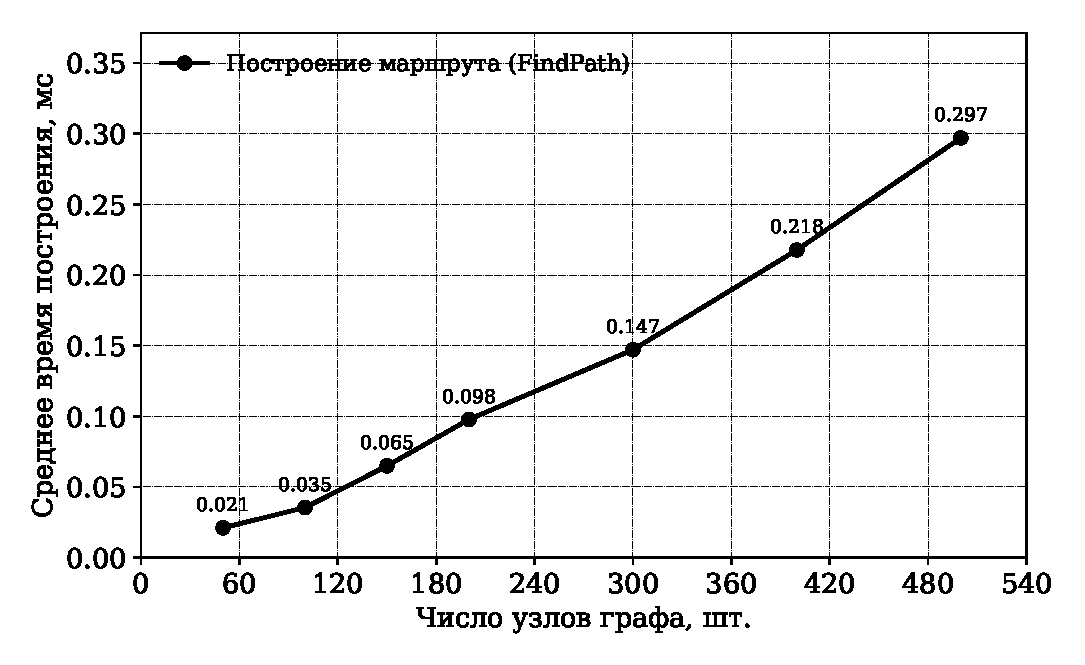
\includegraphics[width=0.85\textwidth]{Pictures/rpperf.eps}
\caption{Зависимость времени построения маршрута от размера графа}
\label{rpperf:image}
\end{figure}

Время выполнения растёт практически линейно с увеличением размера графа, что согласуется с теоретической оценкой сложности $O((V + E) \log V)$ для разреженных графов \cite{cormen}. Все измеренные значения находятся в субмиллисекундном диапазоне и укладываются в установленные требования с многократным запасом: даже на графе из 500~узлов построение маршрута занимает в среднем 0,297~мс при требовании менее 200~мс, а поиск ближайшего эвакуационного выхода -- 0,630~мс при требовании менее 300~мс. Полученный запас по производительности подтверждает пригодность алгоритма Дейкстры для построения маршрутов в реальном времени и оставляет резерв для графов значительно большего объёма.

\subsection{Системное тестирование}

Системное тестирование выполнено для проверки совместной работы всех компонентов приложения IndoorNav в сборе на реальных данных навигационного графа здания (586~узлов, 1202~ребра) и на целевых платформах (Windows, iOS, Android). В отличие от модульного тестирования, проверяющего отдельные методы, системное тестирование оценивает сквозные сценарии <<от действия пользователя до результата на экране>> с участием всех слоёв архитектуры -- представления, модели представления, сервисов и модели данных.

Ниже подробно описаны сквозные сценарии системного тестирования. Для каждого сценария приведены выполняемые действия и полученный результат, а для сценариев, проверенных в работающем приложении, -- снимок экрана.

\subsubsection{Построение маршрута между аудиториями}

\textbf{Сценарий.} Пользователь выбирает начальную и конечную аудитории и запускает построение маршрута на реальном графе здания. Система загружает граф, выполняет поиск кратчайшего пути алгоритмом Дейкстры и формирует пошаговые инструкции.

\textbf{Результат.} Построен кратчайший маршрут между аудиториями, отображён на плане этажа; сформированы пошаговые инструкции. Результат соответствует требованию построения маршрута между точками и показан на рисунке~\ref{rproute:image}.

\begin{figure}[H]
\centering
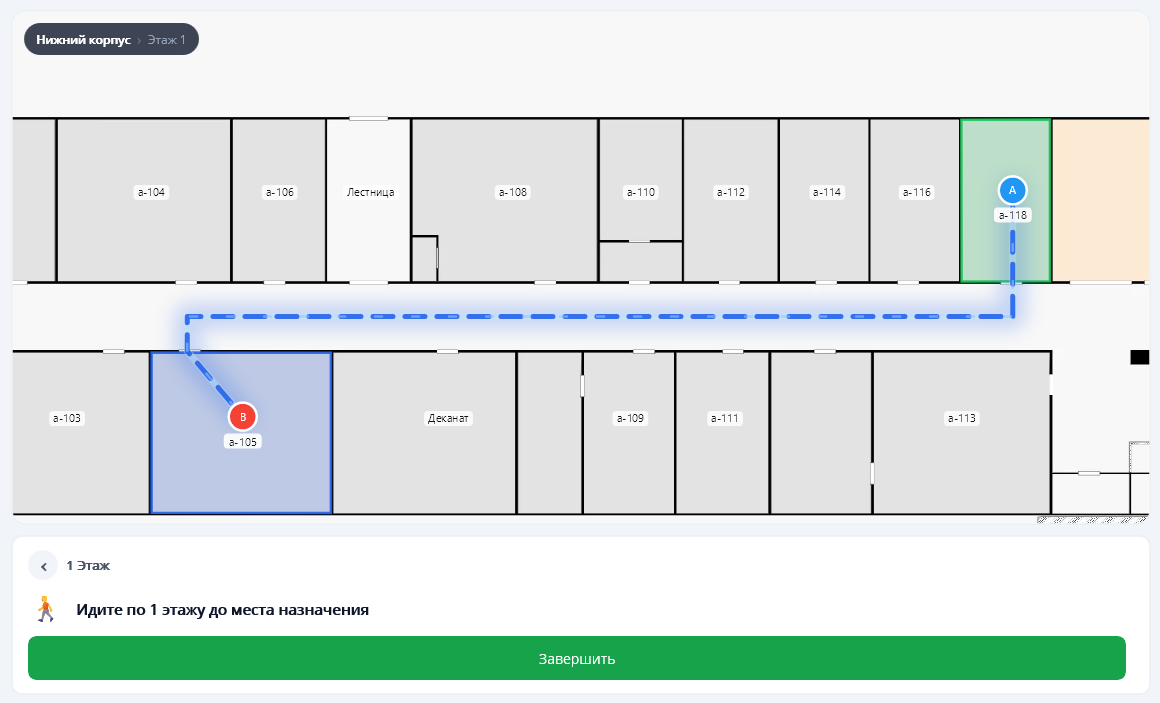
\includegraphics[width=0.95\textwidth]{Pictures/rproute.png}
\caption{Построение маршрута между аудиториями}
\label{rproute:image}
\end{figure}

\subsubsection{Эвакуационный маршрут в режиме ЧС}

\textbf{Сценарий.} Администратор активирует режим чрезвычайной ситуации, после чего система автоматически строит маршрут до ближайшего эвакуационного выхода от текущего положения пользователя.

\textbf{Результат.} Построен маршрут до ближайшего выхода. Результат соответствует требованию работы режима ЧС и показан на рисунке~\ref{rpemergency:image}.

\begin{figure}[H]
\centering
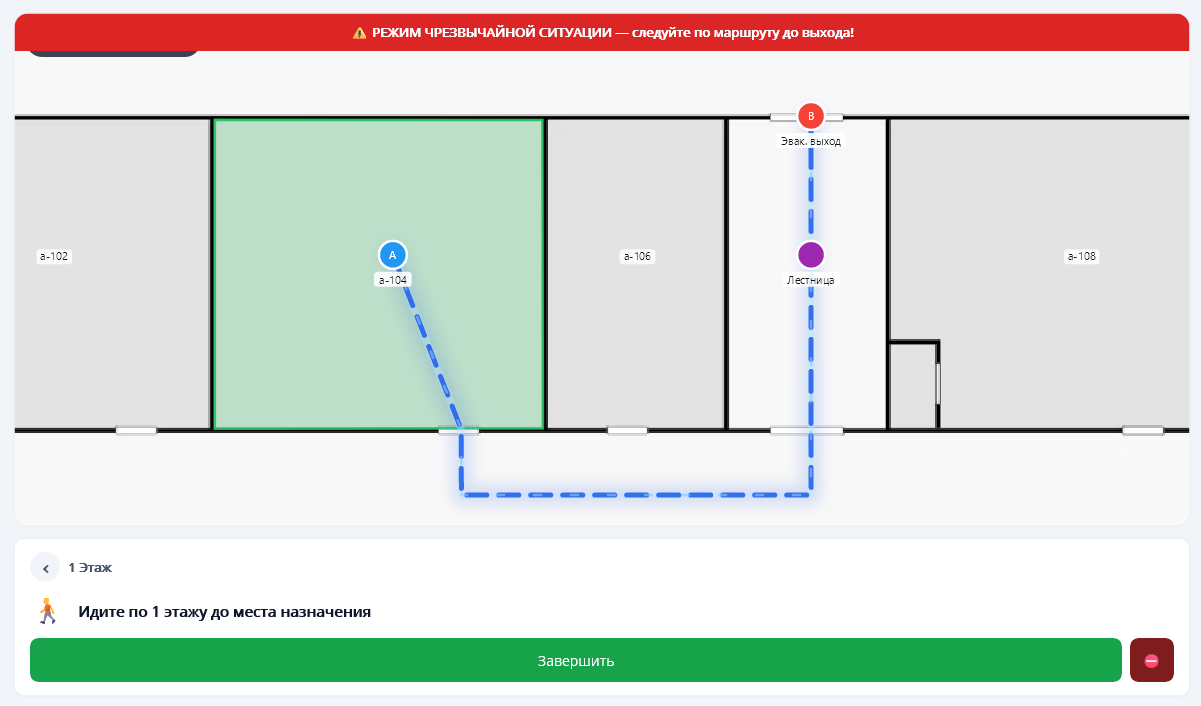
\includegraphics[width=0.95\textwidth]{Pictures/rpemergency.png}
\caption{Эвакуационный маршрут до ближайшего выхода в режиме ЧС}
\label{rpemergency:image}
\end{figure}

\subsubsection{Перестроение маршрута при блокировке}

\textbf{Сценарий.} Пользователь отмечает заблокированный узел на текущем маршруте, после чего система перестраивает путь.

\textbf{Результат.} Маршрут автоматически перестроен в обход заблокированного участка без перезагрузки графа. Результат подтверждает работу механизма динамического исключения узлов и показан на рисунке~\ref{rpreroute:image}.

\begin{figure}[H]
\centering
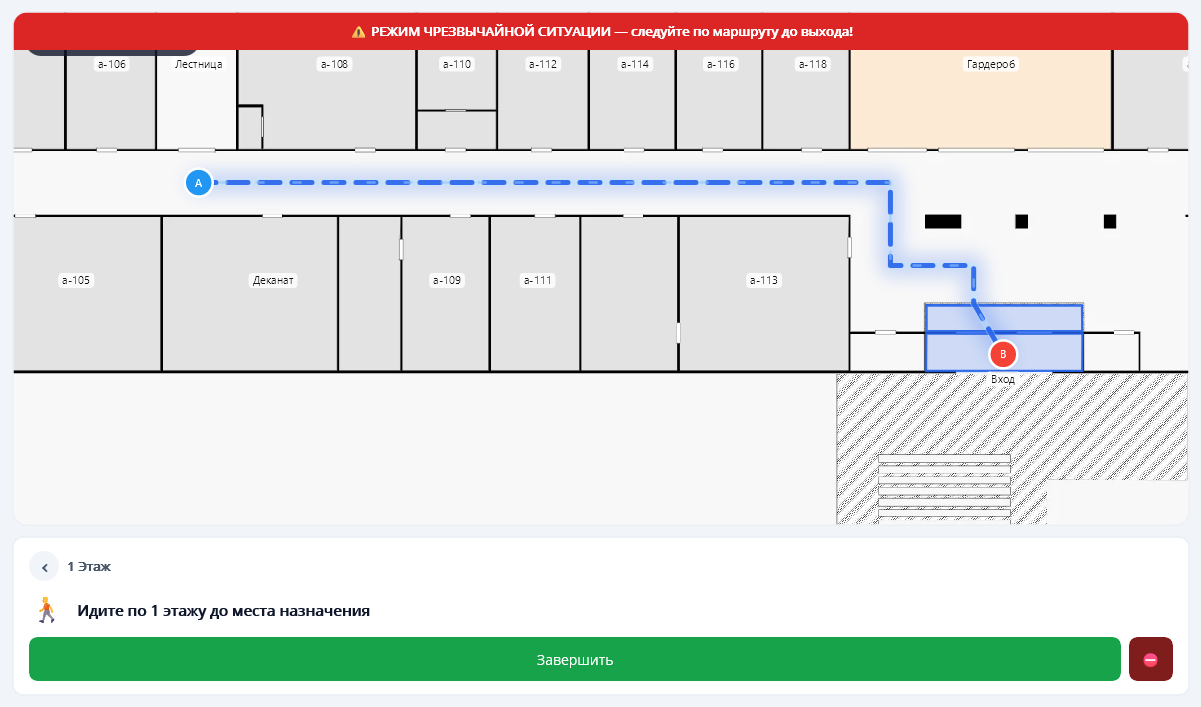
\includegraphics[width=0.95\textwidth]{Pictures/rpreroute.png}
\caption{Перестроение маршрута при блокировке участка}
\label{rpreroute:image}
\end{figure}

\subsubsection{Позиционирование пользователя по QR-коду}

\textbf{Сценарий.} Пользователь сканирует QR-код, размещённый на стене здания. Приложение разбирает ссылку вида \texttt{indoornav://node/\{id\}}, устанавливает соответствующий узел как начальную точку.

\textbf{Результат.} Начальная точка маршрута корректно определена по отсканированному QR-коду. Результат подтверждает интеграцию модуля разбора ссылок с алгоритмом маршрутизации и показан на рисунке~\ref{rpsys2:image}.

\begin{figure}[H]
	\centering
	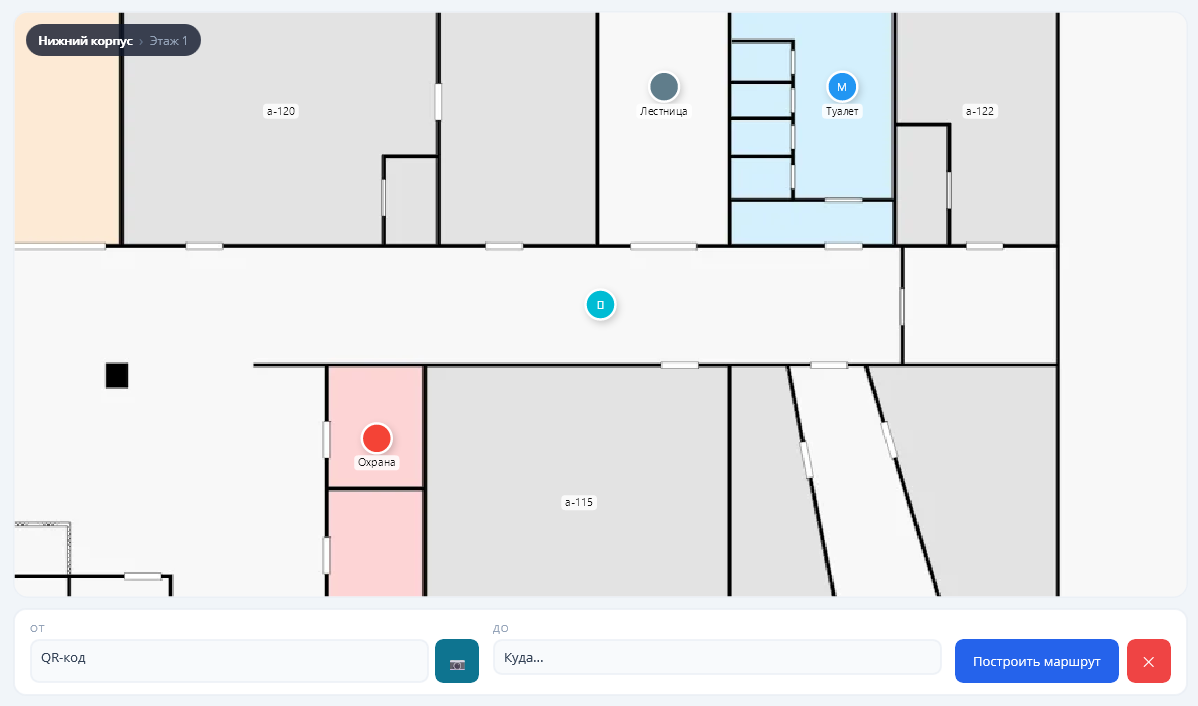
\includegraphics[width=0.95\textwidth]{Pictures/rpsys2.png}
	\caption{Позиционирование пользователя по QR-коду}
	\label{rpsys2:image}
\end{figure}

\subsubsection{Определение исходной точки по расписанию в режиме ЧС}

\textbf{Сценарий.} В здании активирован режим чрезвычайной ситуации. При входе студента в приложение система запрашивает подтверждение того, что он находится в аудитории согласно своему расписанию. При подтверждении эта аудитория автоматически устанавливается как исходная точка, и сразу строится маршрут до ближайшего эвакуационного выхода.

\textbf{Результат.} Исходная точка маршрута определена по подтверждённой аудитории из расписания без ручного выбора, эвакуационный маршрут до ближайшего выхода построен автоматически. Результат подтверждает совместную работу сервиса расписания и модуля эвакуационной маршрутизации и показан на рисунке~\ref{rpsys3:image}.

\begin{figure}[H]
	\centering
	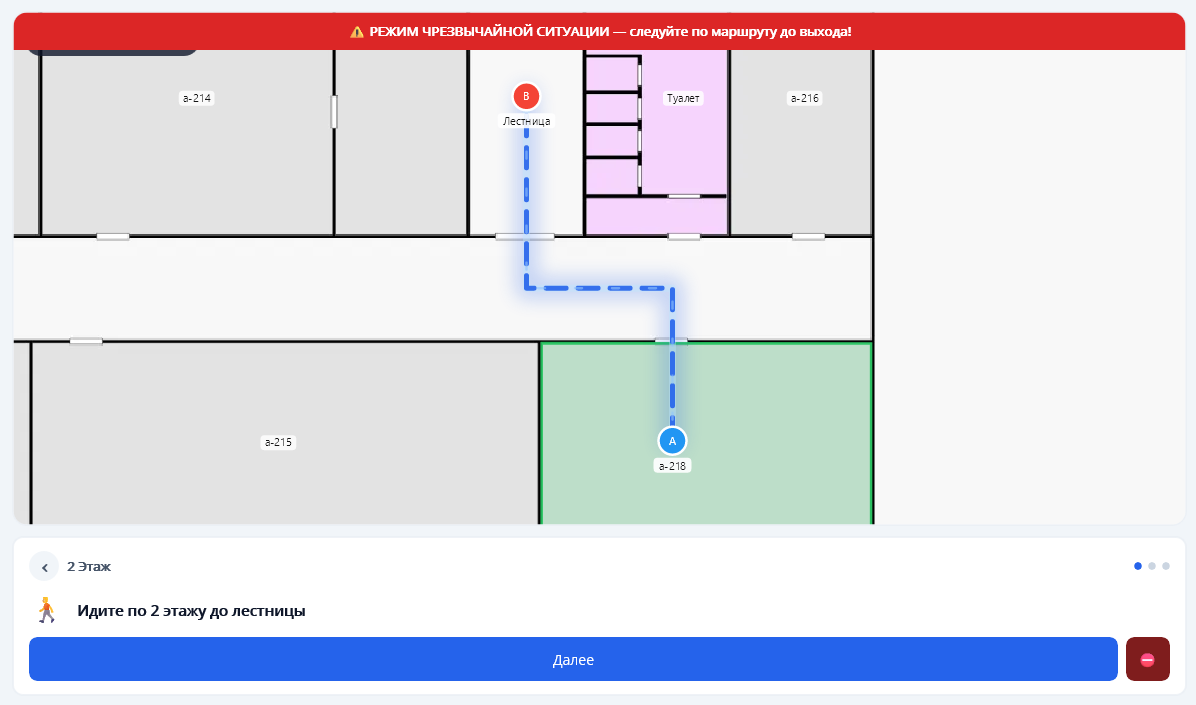
\includegraphics[width=0.95\textwidth]{Pictures/rpsys3.png}
	\caption{Определение исходной точки по расписанию в режиме ЧС}
	\label{rpsys3:image}
\end{figure}

Системное тестирование подтвердило корректную совместную работу всех слоёв приложения на реальных данных графа здания и на целевых платформах.


   % !TeX root = mainstarkov.tex
% !TeX program = xelatex
% !TeX encoding = UTF-8
\section*{ЗАКЛЮЧЕНИЕ}
\addcontentsline{toc}{section}{ЗАКЛЮЧЕНИЕ}

В рамках выпускной квалификационной работы выполнена программная реализация и тестирование алгоритмов динамической маршрутизации для системы построения эвакуационных маршрутов в замкнутых пространствах. Все поставленные задачи решены в полном объёме.

Проведён анализ существующих алгоритмов поиска кратчайших путей на графах. На основании сравнительного анализа по критериям оптимальности, производительности, поддержки динамического исключения узлов и сложности реализации выбран алгоритм Дейкстры как наилучшее решение для задачи эвакуационной маршрутизации. Алгоритм обеспечивает гарантию оптимальности при неотрицательных весах рёбер, эффективную работу на разреженных графах, характерных для планов зданий, и допускает модификацию для динамического исключения заблокированных узлов.

Разработаны структуры данных для представления навигационного графа: классы \texttt{NavGraph}, \texttt{NavNode} и \texttt{NavEdge}, обеспечивающие эффективное хранение и обработку топологии здания. Класс \texttt{NavNode} содержит полный набор атрибутов узла: координаты, номер этажа, идентификатор здания, флаги типа и группу перехода. Класс \texttt{NavEdge} хранит вес ребра с автоматическим вычислением евклидова расстояния для проходов. Реализована загрузка и сохранение графа в формате JSON средствами \texttt{System.Text.Json}.

Реализован алгоритм Дейкстры с модификациями для поддержки динамического исключения узлов. Множество исключённых узлов передаётся как параметр метода \texttt{FindPath} и проверяется при релаксации рёбер без модификации исходного графа. Конечный узел маршрута никогда не исключается. Алгоритм использует стандартные структуры данных .NET (\texttt{SortedSet}, \texttt{Dictionary}, \texttt{HashSet}) и обеспечивает время выполнения менее 200 мс для графов до 500 узлов, что соответствует требованиям реального времени. Оптимизация списка смежности и обработка устаревших записей очереди повышают эффективность реализации.

Разработан алгоритм поиска ближайшего эвакуационного выхода, учитывающий текущее положение пользователя, принадлежность к зданию и динамически изменяющиеся препятствия. Алгоритм приоритизирует выходы в текущем здании. Алгоритм интегрирован с сервисом экстренной эвакуации \texttt{EmergencyService} и ViewModel приложения IndoorNav.

Разработан механизм формирования множества исключённых узлов \texttt{BuildExcludeSet}, объединяющий заблокированные пользователем узлы и выходы, не являющиеся целевыми. Это предотвращает прохождение маршрута через другие выходы и обеспечивает корректное перестроение маршрута при блокировке участков.

Проведено комплексное тестирование алгоритмической части: модульное тестирование четырёх модулей маршрутизации (построение маршрута, поиск эвакуационного выхода, вычисление весов рёбер и формирование множества исключений), тестирование производительности на графах от 50 до 500 узлов, а также интеграционное тестирование на реальных данных графа здания университета. Результаты подтвердили корректность работы алгоритмов во всех сценариях, включая граничные случаи (пустой граф, несвязный граф, совпадение стартовой и конечной точек), и соответствие требованиям производительности.

Таким образом, в ходе выпускной квалификационной работы реализованы и верифицированы алгоритмы динамической маршрутизации для системы построения эвакуационных маршрутов в замкнутых пространствах. Полученные результаты могут быть применены в навигационных системах внутри зданий, приложениях экстренной эвакуации и иных программных комплексах, требующих эффективного построения маршрутов с учётом динамических ограничений. Дальнейшее развитие системы может включать реализацию алгоритма A* с допустимой эвристикой, поддержку двунаправленного поиска и интеграцию с серверной частью для распределённого построения маршрутов.

}{\else{
   % !TeX root = mainstarkov.tex
% !TeX program = xelatex
% !TeX encoding = UTF-8
\section{Рабочий проект}

\subsection{Общая характеристика рабочего проекта}

Если в техническом проекте приведены проектные решения и псевдокод алгоритмов динамической маршрутизации, то в рабочем проекте представлена их программная реализация на языке C\# в составе приложения IndoorNav и результаты комплексного тестирования. Реализация выполнена в соответствии с проектными решениями технического проекта (таблица~\ref{algreq:table}) и сохраняет принцип разделения ответственности: структуры данных, алгоритмы поиска пути и логика эвакуации реализованы как независимые модули, что обеспечивает возможность их раздельного тестирования.

В процессе разработки алгоритмического ядра динамической маршрутизации выделены следующие программные модули: \texttt{NavNode}, \texttt{NavEdge}, \texttt{NavGraph}, \texttt{NavGraphService}, \texttt{EmergencyService} и \texttt{MainViewModel}. Их состав и распределение по слоям архитектуры приведены в таблице~\ref{rpfiles:table}.

\begin{xltabular}{\textwidth}{|l|c|X|}
\caption{Состав программных модулей алгоритмического ядра\label{rpfiles:table}}\\ \hline
\centrow Модуль (файл) & \centrow Слой & \centrow Назначение \\ \hline
\thead{1} & \thead{2} & \centrow 3 \\ \hline
\endfirsthead
\continuecaption{Продолжение таблицы \ref{rpfiles:table}}
\centrow Модуль (файл) & \centrow Слой & \centrow Назначение \\ \hline
\finishhead
\texttt{NavNode.cs} & Model & Класс узла навигационного графа \\ \hline
\texttt{NavEdge.cs} & Model & Класс ребра графа с весом \\ \hline
\texttt{NavGraph.cs} & Model & Граф и алгоритм Дейкстры (\texttt{FindPath}) \\ \hline
\texttt{NavGraphService.cs} & Service & Загрузка, сохранение и предоставление графа \\ \hline
\texttt{EmergencyService.cs} & Service & Поиск ближайшего эвакуационного выхода \\ \hline
\texttt{MainViewModel.cs} & ViewModel & Построение маршрута, множество исключений, пошаговые инструкции
\end{xltabular}

Далее каждый модуль рассмотрен отдельно: приведены его назначение и таблица реализованных полей или методов с описанием параметров.

\subsection{Модули данных NavNode и NavEdge}

\texttt{NavNode} -- класс узла навигационного графа, представляющий точку на плане этажа (помещение, коридор, перекрёсток, лестничную площадку или выход). \texttt{NavEdge} -- класс ребра графа, представляющий проход между двумя узлами с весом. Это модули данных без вычислительной логики; их ключевые поля приведены в таблицах~\ref{rpnode:table} и~\ref{rpedge:table}.

\begin{xltabular}{\textwidth}{|l|l|X|}
\caption{Ключевые поля класса NavNode\label{rpnode:table}}\\ \hline
\centrow Поле & \centrow Тип & \centrow Описание \\ \hline
\thead{1} & \thead{2} & \centrow 3 \\ \hline
\endfirsthead
\continuecaption{Продолжение таблицы \ref{rpnode:table}}
\centrow Поле & \centrow Тип & \centrow Описание \\ \hline
\finishhead
\texttt{Id} & string & Уникальный идентификатор узла \\ \hline
\texttt{X}, \texttt{Y} & float & Координаты узла на плане этажа \\ \hline
\texttt{FloorNumber} & int & Номер этажа \\ \hline
\texttt{BuildingId} & string & Идентификатор здания (корпуса) \\ \hline
\texttt{IsTransition} & bool & Узел межэтажного перехода (лестница, лифт) \\ \hline
\texttt{IsExit} & bool & Основной выход из здания \\ \hline
\texttt{IsEvacuationExit} & bool & Эвакуационный выход \\ \hline
\texttt{TransitionGroupId} & string & Группа перехода для связывания узлов разных этажей
\end{xltabular}

\begin{xltabular}{\textwidth}{|l|l|X|}
\caption{Поля класса NavEdge\label{rpedge:table}}\\ \hline
\centrow Поле & \centrow Тип & \centrow Описание \\ \hline
\endfirsthead
\continuecaption{Продолжение таблицы \ref{rpedge:table}}
\centrow Поле & \centrow Тип & \centrow Описание \\ \hline
\finishhead
\texttt{FromId}, \texttt{ToId} & string & Идентификаторы соединяемых узлов \\ \hline
\texttt{Weight} & float & Вес ребра (евклидово расстояние или штраф 150) \\ \hline
\texttt{IsCrossFloor} & bool & Признак межэтажного ребра
\end{xltabular}

\subsection{Модуль NavGraph}

\texttt{NavGraph} -- центральный модуль алгоритмического ядра: хранит коллекции узлов и рёбер и реализует поиск кратчайшего пути по алгоритму Дейкстры с поддержкой динамического исключения узлов. Описание реализованных методов приведено в таблице~\ref{rpgraph:table}.

\begin{xltabular}{\textwidth}{|X|X|X|}
\caption{Методы модуля NavGraph\label{rpgraph:table}}\\ \hline
\centrow Метод & \centrow Аргументы & \centrow Описание \\ \hline
\thead{1} & \thead{2} & \centrow 3 \\ \hline
\endfirsthead
\continuecaption{Продолжение таблицы \ref{rpgraph:table}}
\centrow Метод & \centrow Аргументы & \centrow Описание \\ \hline
\finishhead
\texttt{GetNode} & \texttt{id} & Возвращает узел по идентификатору или \texttt{null} \\ \hline
\texttt{FindPath} & \texttt{startId}, \texttt{endId}, \texttt{excludeIds} & Поиск кратчайшего пути по алгоритму Дейкстры с динамическим исключением узлов \\ \hline
\texttt{AddEdge} & \texttt{fromId}, \texttt{toId}, \texttt{crossFloor} & Добавление ребра с автоматическим вычислением веса в обоих направлениях \\ \hline
\texttt{RemoveEdge} & \texttt{fromId}, \texttt{toId} & Удаление ребра между двумя узлами \\ \hline
\texttt{EdgeExists} & \texttt{fromId}, \texttt{toId} & Проверка наличия ребра между узлами \\ \hline
\texttt{GetNodesForFloor} & \texttt{buildingId}, \texttt{floor} & Узлы заданного этажа корпуса \\ \hline
\texttt{GetEdgesForFloor} & \texttt{buildingId}, \texttt{floor} & Рёбра заданного этажа корпуса
\end{xltabular}

Реализация поиска кратчайшего пути по алгоритму Дейкстры в методе \texttt{FindPath} принимает на вход идентификаторы стартового и конечного узлов, а также множество исключаемых узлов \texttt{excludeIds}. Пример:


\begin{figure}[H]
\begin{lstlisting}[language={[Sharp]C}]
public List<NavNode> FindPath(string startId, string endId, ISet<string>? excludeIds)
{
    if (startId == endId)
        return GetNode(startId) is { } n ? [n] : [];

    var dist  = new Dictionary<string, float>();
    var prev  = new Dictionary<string, string?>();
    var queue = new SortedSet<(float dist, string id)>(
        Comparer<(float, string)>.Create((a, b) =>
            a.Item1 != b.Item1 ? a.Item1.CompareTo(b.Item1)
                               : string.Compare(a.Item2, b.Item2, StringComparison.Ordinal)));

    foreach (var node in Nodes)            
    {
        dist[node.Id] = float.MaxValue;
        prev[node.Id] = null;
    }
    dist[startId] = 0;
    queue.Add((0, startId));

    var adj = Nodes.ToDictionary(n => n.Id, _ => new List<(string neighbor, float weight)>());
    foreach (var edge in Edges)
        if (adj.ContainsKey(edge.FromId))
            adj[edge.FromId].Add((edge.ToId, edge.Weight));

    while (queue.Count > 0)
    {
        var (d, u) = queue.Min;            
        queue.Remove(queue.Min);
        if (u == endId) break;
        if (d > dist[u]) continue;         

        foreach (var (v, w) in adj[u])     
        {
            if (excludeIds != null && excludeIds.Contains(v) && v != endId) continue;
            float alt = dist[u] + w;
            if (alt < dist[v])
            {
                queue.Remove((dist[v], v));
                dist[v] = alt;
                prev[v] = u;
                queue.Add((alt, v));
            }
        }
    }

    if (dist[endId] == float.MaxValue) return [];
}
\end{lstlisting}
\end{figure}

Очередь с приоритетом реализована на основе \texttt{SortedSet} с компаратором, сравнивающим элементы сначала по расстоянию, а при равенстве -- по идентификатору узла. Это гарантирует строгий порядок элементов и детерминированность результата. Список смежности \texttt{adj} строится один раз перед основным циклом, что обеспечивает доступ к соседям вершины за константное время. Устаревшие записи очереди не удаляются при обновлении расстояния, а отбрасываются при извлечении проверкой \texttt{d > dist[u]}.

\subsection{Модуль NavGraphService}

\texttt{NavGraphService} -- сервисный модуль, отвечающий за загрузку, сохранение и предоставление навигационного графа, а также за операции добавления и удаления узлов и рёбер. Сериализация графа выполняется средствами \texttt{System.Text.Json}. Описание методов приведено в таблице~\ref{rpsvc:table}.

\begin{xltabular}{\textwidth}{|X|X|X|}
\caption{Методы модуля NavGraphService\label{rpsvc:table}}\\ \hline
\centrow Метод & \centrow Аргументы & \centrow Описание \\ \hline
\thead{1} & \thead{2} & \centrow 3 \\ \hline
\endfirsthead
\continuecaption{Продолжение таблицы \ref{rpsvc:table}}
\centrow Метод & \centrow Аргументы & \centrow Описание \\ \hline
\finishhead
\texttt{LoadAsync} & -- & Загрузка графа из файла \texttt{navgraph.json} \\ \hline
\texttt{SaveAsync} & -- & Сохранение графа в файл \texttt{navgraph.json} \\ \hline
\texttt{ResetAsync} & -- & Сброс графа и удаление файла данных \\ \hline
\texttt{AddNode} & \texttt{node} & Добавление узла в граф \\ \hline
\texttt{RemoveNode} & \texttt{id} & Удаление узла вместе с инцидентными рёбрами \\ \hline
\texttt{AddEdge} & \texttt{fromId}, \texttt{toId}, \texttt{crossFloor} & Добавление ребра в граф \\ \hline
\texttt{RemoveEdge} & \texttt{fromId}, \texttt{toId} & Удаление ребра из графа
\end{xltabular}

\subsection{Модуль EmergencyService}

\texttt{EmergencyService} -- сервисный модуль режима чрезвычайной ситуации: управляет состоянием ЧС по зданиям и реализует поиск кратчайшего пути до ближайшего эвакуационного выхода. Описание методов приведено в таблице~\ref{rpemerg:table}.

\begin{xltabular}{\textwidth}{|X|X|X|}
\caption{Методы модуля EmergencyService\label{rpemerg:table}}\\ \hline
\centrow Метод & \centrow Аргументы & \centrow Описание \\ \hline
\thead{1} & \thead{2} & \centrow 3 \\ \hline
\endfirsthead
\continuecaption{Продолжение таблицы \ref{rpemerg:table}}
\centrow Метод & \centrow Аргументы & \centrow Описание \\ \hline
\finishhead
\texttt{FindNearestExitRoute} & \texttt{start}, \texttt{graph}, \texttt{excludeIds} & Поиск пути до ближайшего эвакуационного выхода \\ \hline
\texttt{Activate} & \texttt{buildingId} & Активация режима ЧС для здания \\ \hline
\texttt{Deactivate} & \texttt{buildingId} & Отключение режима ЧС для здания \\ \hline
\texttt{ActivateAll} & \texttt{buildingIds} & Активация ЧС для всех зданий \\ \hline
\texttt{IsActiveForBuilding} & \texttt{buildingId} & Проверка активности ЧС для здания \\ \hline
\texttt{LoadAsync} & -- & Восстановление состояния ЧС из файла
\end{xltabular}

Реализация поиска ближайшего эвакуационного выхода выполнена в методе \texttt{FindNearestExitRoute}: он отбирает множество узлов-выходов, запускает однократный обход Дейкстры от стартовой точки и выбирает выход с минимальным расстоянием. Пример:

\begin{figure}[H]
\begin{lstlisting}[language={[Sharp]C}]
var exits = graph.Nodes
    .Where(n => (n.IsExit || n.IsEvacuationExit)
                && n.BuildingId == start.BuildingId
                && excludeIds?.Contains(n.Id) != true)
    .ToList();

var bestExit = exits.OrderBy(e => dist.GetValueOrDefault(e.Id, double.MaxValue))
                    .FirstOrDefault();
	if (bestExit == null || dist[bestExit.Id] == double.MaxValue) return new();

var path = new List<NavNode>();
string? cur = bestExit.Id;
	while (cur != null)
		{
		    if (nodeMap.TryGetValue(cur, out var node)) path.Add(node);
		    prev.TryGetValue(cur, out cur);
		}
path.Reverse();
return path;
\end{lstlisting}
\end{figure}

Приоритизация выходов текущего здания исключает построение маршрута в соседний корпус при наличии ближайшего выхода. Резервный поиск по всем корпусам гарантирует нахождение выхода в нестандартной конфигурации данных. Заблокированные узлы исключаются на этапе отбора выходов и при релаксации рёбер.

\subsection{Модуль MainViewModel}

\texttt{MainViewModel} -- модуль слоя представления, связывающий пользовательский интерфейс с алгоритмами маршрутизации: формирует множество исключаемых узлов, вызывает построение маршрута и формирует пошаговые инструкции. Описание ключевых методов приведено в таблице~\ref{rpvm:table}.

\begin{xltabular}{\textwidth}{|X|X|X|}
\caption{Ключевые методы модуля MainViewModel\label{rpvm:table}}\\ \hline
\centrow Метод & \centrow Аргументы & \centrow Описание \\ \hline
\thead{1} & \thead{2} & \centrow 3 \\ \hline
\endfirsthead
\continuecaption{Продолжение таблицы \ref{rpvm:table}}
\centrow Метод & \centrow Аргументы & \centrow Описание \\ \hline
\finishhead
\texttt{ExecuteBuildRoute} & -- & Построение маршрута между выбранными точками \\ \hline
\texttt{ExecuteBuildEmergencyRoute} & -- & Построение эвакуационного маршрута в режиме ЧС \\ \hline
\texttt{BuildExcludeSet} & \texttt{startId}, \texttt{endId} & Формирование множества исключаемых узлов \\ \hline
\texttt{BuildRouteSteps} & \texttt{path} & Формирование пошаговых инструкций по маршруту
\end{xltabular}

Формирование множества исключаемых узлов выполняется методом \texttt{BuildExcludeSet}, объединяющим выходы, не являющиеся целевыми, и узлы, заблокированные пользователем.

\begin{figure}[H]
\begin{lstlisting}[language={[Sharp]C}]
private HashSet<string> BuildExcludeSet(string startId, string endId)
{
    var exclude = new HashSet<string>();
    foreach (var n in _graph.Nodes)
        if ((n.IsExit || n.IsEvacuationExit) && n.Id != startId && n.Id != endId)
            exclude.Add(n.Id);
    foreach (var id in _blockedNodeIds)
        exclude.Add(id);
    return exclude;
}
\end{lstlisting}
\end{figure}

Объединение двух источников исключений в одном множестве позволяет единообразно передавать ограничения в метод \texttt{FindPath} и обеспечивает автоматическое перестроение маршрута в обход заблокированных участков.

\subsection{Модульное тестирование}

Для проверки корректности разработаны модульные тесты для четырёх модулей, образующих алгоритмическое ядро маршрутизации: построения маршрута (\texttt{NavGraph.FindPath}), поиска ближайшего эвакуационного выхода (\texttt{EmergencyService.FindNearestExitRoute}), вычисления весов рёбер (\texttt{NavGraph.AddEdge}) и формирования множества исключений (\texttt{MainViewModel.BuildExcludeSet}). Для каждого модуля составлена отдельная таблица тестовых наборов, в которой указаны сценарий, входные данные и эталонный выходной результат.

\subsubsection{Тестирование модуля построения маршрута}

Тестовые наборы для модуля построения маршрута охватывают типовые и граничные сценарии и приведены в таблице~\ref{rpunit:table}. Пример реализации теста построения простого маршрута на линейном графе приведён ниже.

\begin{figure}[H]
\begin{lstlisting}[language={[Sharp]C}]
[Test]
public void FindPath_LinearGraph_ReturnsFullPath()
{
    var graph = new NavGraph();
    graph.Nodes.Add(new NavNode { Id = "A", X = 0, Y = 0 });
    graph.Nodes.Add(new NavNode { Id = "B", X = 10, Y = 0 });
    graph.Nodes.Add(new NavNode { Id = "C", X = 20, Y = 0 });
    graph.AddEdge("A", "B");
    graph.AddEdge("B", "C");

    var path = graph.FindPath("A", "C", null);

    Assert.AreEqual(3, path.Count);
    Assert.AreEqual("A", path.First().Id);
    Assert.AreEqual("C", path.Last().Id);
}
\end{lstlisting}
\end{figure}

\begin{xltabular}{\textwidth}{|c|X|X|X|}
\caption{Тестовые наборы для модуля построения маршрута (NavGraph.FindPath)\label{rpunit:table}}\\ \hline
\centrow № & \centrow Сценарий & \centrow Входные данные & \centrow Эталонные выходные данные \\ \hline
\thead{1} & \thead{2} & \thead{3} & \centrow 4 \\ \hline
\endfirsthead
\continuecaption{Продолжение таблицы \ref{rpunit:table}}
\centrow № & \centrow Сценарий & \centrow Входные данные & \centrow Эталонные выходные данные \\ \hline
\finishhead
1 & Простой маршрут & Линейный граф из узлов A, B, C; запрос A$\to$C & Путь из трёх узлов [A, B, C] \\ \hline
2 & Выбор оптимального пути & Граф с двумя ветвями разной длины & Кратчайшая из ветвей \\ \hline
3 & Граф с циклом & Граф, содержащий цикл & Кратчайший путь без зацикливания \\ \hline
4 & Несуществующий узел & Отсутствующий стартовый или конечный идентификатор & Пустой список \\ \hline
5 & Исключение узла & Множество исключений с одним промежуточным узлом & Маршрут в обход исключённого узла \\ \hline
6 & Полная блокировка пути & В множество исключений добавлены все промежуточные узлы & Пустой список \\ \hline
7 & Старт совпадает с целью & Стартовый и конечный узел совпадают & Список из одного узла \\ \hline
8 & Межэтажный переход & Граф с межэтажным ребром (вес 150) & Путь с учётом штрафного веса 150 \\ \hline
9 & Последовательное исключение & Повторные вызовы с растущим множеством исключений & Корректно перестроенный маршрут \\ \hline
10 & Исключение конечного узла & Конечный узел добавлен в множество исключений & Конечный узел достижим, путь построен \\ \hline
11 & Пустой граф & Граф без узлов & Пустой список \\ \hline
12 & Несвязный граф & Старт и цель в разных компонентах связности & Пустой список
\end{xltabular}

\subsubsection{Тестирование модуля поиска эвакуационного выхода}

Тестовые наборы для модуля поиска ближайшего эвакуационного выхода учитывают приоритет выходов текущего здания, резервный поиск по всем корпусам и исключение заблокированных выходов; они приведены в таблице~\ref{rpexit:table}.

\begin{xltabular}{\textwidth}{|c|X|X|X|}
\caption{Тестовые наборы для модуля поиска эвакуационного выхода (EmergencyService.FindNearestExitRoute)\label{rpexit:table}}\\ \hline
\centrow № & \centrow Сценарий & \centrow Входные данные & \centrow Эталонные выходные данные \\ \hline
\thead{1} & \thead{2} & \thead{3} & \centrow 4 \\ \hline
\endfirsthead
\continuecaption{Продолжение таблицы \ref{rpexit:table}}
\centrow № & \centrow Сценарий & \centrow Входные данные & \centrow Эталонные выходные данные \\ \hline
\finishhead
1 & Несколько выходов & Граф с двумя и более выходами; стартовый узел & Путь до ближайшего выхода \\ \hline
2 & Единственный выход & Граф с одним узлом-выходом & Путь до этого выхода \\ \hline
3 & Нет выходов & Граф без узлов-выходов & Пустой список \\ \hline
4 & Выход в другом корпусе & В текущем здании выходов нет & Путь до выхода другого корпуса (резервный поиск) \\ \hline
5 & Заблокированный выход & Ближайший выход добавлен в множество исключений & Путь до следующего по близости выхода
\end{xltabular}

\subsubsection{Тестирование модуля вычисления весов рёбер}

Модуль вычисления весов рёбер (\texttt{NavGraph.AddEdge}) формирует вес ребра как евклидово расстояние между узлами одного этажа либо как фиксированный штраф 150 для межэтажных переходов и добавляет ребро в обоих направлениях. От корректности весов напрямую зависит оптимальность маршрутов, поэтому модуль тестируется отдельно. Тестовые наборы приведены в таблице~\ref{rpweight:table}.

\begin{xltabular}{\textwidth}{|c|X|X|X|}
\caption{Тестовые наборы для модуля вычисления весов рёбер (NavGraph.AddEdge)\label{rpweight:table}}\\ \hline
\centrow № & \centrow Сценарий & \centrow Входные данные & \centrow Эталонные выходные данные \\ \hline
\thead{1} & \thead{2} & \thead{3} & \centrow 4 \\ \hline
\endfirsthead
\continuecaption{Продолжение таблицы \ref{rpweight:table}}
\centrow № & \centrow Сценарий & \centrow Входные данные & \centrow Эталонные выходные данные \\ \hline
\finishhead
1 & Вес горизонтального ребра & Узлы с координатами (0, 0) и (3, 4) на одном этаже & Вес ребра = 5,0 (евклидово расстояние) \\ \hline
2 & Вес межэтажного ребра & Добавление ребра с признаком межэтажного перехода & Вес ребра = 150 \\ \hline
3 & Двунаправленность ребра & Добавление ребра между узлами A и B & Создаются рёбра A$\to$B и B$\to$A с равным весом \\ \hline
4 & Защита от дублирования & Повторное добавление уже существующего ребра & Повторное ребро не создаётся \\ \hline
5 & Несуществующий узел & Добавление ребра с отсутствующим идентификатором узла & Ребро не создаётся
\end{xltabular}

\subsubsection{Тестирование модуля формирования множества исключений}

Модуль формирования множества исключений (\texttt{MainViewModel.BuildExcludeSet}) объединяет узлы-выходы, не являющиеся целевыми, и заблокированные пользователем узлы; именно он обеспечивает динамическое перестроение маршрута в обход недоступных участков. Тестовые наборы приведены в таблице~\ref{rpexcl:table}.

\begin{xltabular}{\textwidth}{|c|X|X|X|}
\caption{Тестовые наборы для модуля формирования множества исключений (MainViewModel.BuildExcludeSet)\label{rpexcl:table}}\\ \hline
\centrow № & \centrow Сценарий & \centrow Входные данные & \centrow Эталонные выходные данные \\ \hline
\thead{1} & \thead{2} & \thead{3} & \centrow 4 \\ \hline
\endfirsthead
\continuecaption{Продолжение таблицы \ref{rpexcl:table}}
\centrow № & \centrow Сценарий & \centrow Входные данные & \centrow Эталонные выходные данные \\ \hline
\finishhead
1 & Исключение прочих выходов & Граф с несколькими выходами; старт и цель не являются выходами & В множество включены все узлы-выходы \\ \hline
2 & Стартовый выход не исключается & Стартовый узел помечен как выход & Стартовый узел отсутствует в множестве \\ \hline
3 & Целевой выход не исключается & Конечный узел помечен как выход & Конечный узел отсутствует в множестве \\ \hline
4 & Учёт заблокированных узлов & Список заблокированных узлов содержит узел X & Узел X включён в множество \\ \hline
5 & Объединение источников & Заданы и узлы-выходы, и заблокированные узлы & Множество = выходы (кроме старта и цели) и заблокированные узлы
\end{xltabular}

\subsection{Тестирование производительности}

Для подтверждения соответствия требованиям реального времени проведены замеры времени построения маршрута на графах различного объёма. Замеры выполнены на ПК с процессором AMD Ryzen~7 5700X в среде выполнения .NET~9 (конфигурация Release); для каждого размера графа результат усреднён по 20000 построений маршрута между случайными парами узлов на 5 различных связных разреженных графах. Результаты замеров приведены в таблице~\ref{rpperf:table}, графическая зависимость времени выполнения от размера графа -- на рисунке~\ref{rpperf:image}.

\begin{xltabular}{\textwidth}{|c|c|R|c|}
\caption{Результаты тестирования производительности\label{rpperf:table}}\\ \hline
\centrow Узлы & \centrow Рёбра & \centrow Среднее время, мс & \centrow Требование \\ \hline
\endfirsthead
\continuecaption{Продолжение таблицы \ref{rpperf:table}}
\centrow Узлы & \centrow Рёбра & \centrow Среднее время, мс & \centrow Требование \\ \hline
\finishhead
50 & 80 & 0,021 & $<200$ мс \\ \hline
100 & 160 & 0,035 & $<200$ мс \\ \hline
150 & 250 & 0,065 & $<200$ мс \\ \hline
200 & 350 & 0,098 & $<200$ мс \\ \hline
300 & 520 & 0,147 & $<200$ мс \\ \hline
400 & 700 & 0,218 & $<200$ мс \\ \hline
500 & 900 & 0,297 & $<200$ мс \\ \hline
500 (поиск выхода) & 900 & 0,630 & $<300$ мс
\end{xltabular}

\begin{figure}[H]
\centering
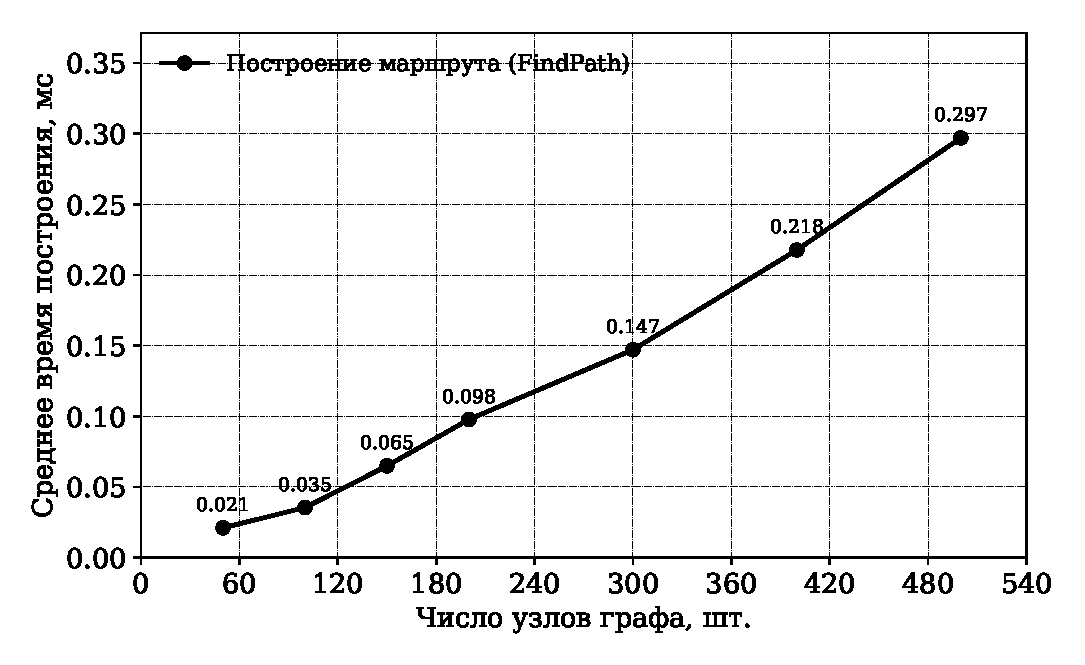
\includegraphics[width=0.85\textwidth]{Pictures/rpperf.eps}
\caption{Зависимость времени построения маршрута от размера графа}
\label{rpperf:image}
\end{figure}

Время выполнения растёт практически линейно с увеличением размера графа, что согласуется с теоретической оценкой сложности $O((V + E) \log V)$ для разреженных графов \cite{cormen}. Все измеренные значения находятся в субмиллисекундном диапазоне и укладываются в установленные требования с многократным запасом: даже на графе из 500~узлов построение маршрута занимает в среднем 0,297~мс при требовании менее 200~мс, а поиск ближайшего эвакуационного выхода -- 0,630~мс при требовании менее 300~мс. Полученный запас по производительности подтверждает пригодность алгоритма Дейкстры для построения маршрутов в реальном времени и оставляет резерв для графов значительно большего объёма.

\subsection{Системное тестирование}

Системное тестирование выполнено для проверки совместной работы всех компонентов приложения IndoorNav в сборе на реальных данных навигационного графа здания (586~узлов, 1202~ребра) и на целевых платформах (Windows, iOS, Android). В отличие от модульного тестирования, проверяющего отдельные методы, системное тестирование оценивает сквозные сценарии <<от действия пользователя до результата на экране>> с участием всех слоёв архитектуры -- представления, модели представления, сервисов и модели данных.

Ниже подробно описаны сквозные сценарии системного тестирования. Для каждого сценария приведены выполняемые действия и полученный результат, а для сценариев, проверенных в работающем приложении, -- снимок экрана.

\subsubsection{Построение маршрута между аудиториями}

\textbf{Сценарий.} Пользователь выбирает начальную и конечную аудитории и запускает построение маршрута на реальном графе здания. Система загружает граф, выполняет поиск кратчайшего пути алгоритмом Дейкстры и формирует пошаговые инструкции.

\textbf{Результат.} Построен кратчайший маршрут между аудиториями, отображён на плане этажа; сформированы пошаговые инструкции. Результат соответствует требованию построения маршрута между точками и показан на рисунке~\ref{rproute:image}.

\begin{figure}[H]
\centering
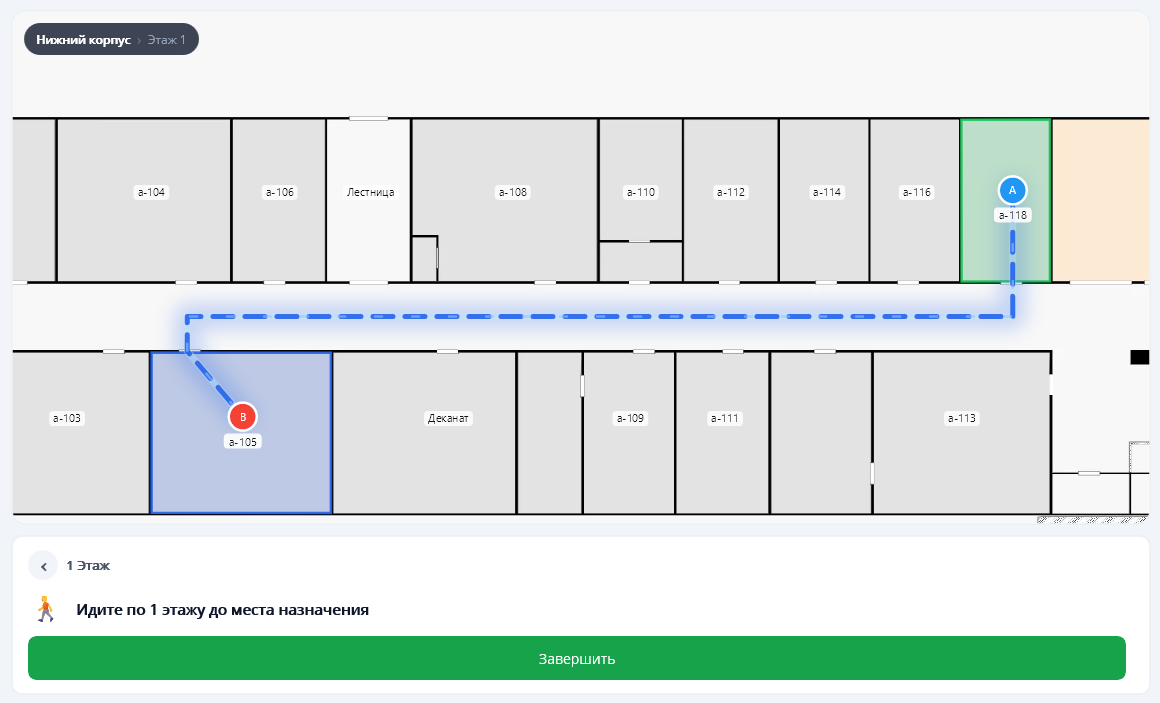
\includegraphics[width=0.95\textwidth]{Pictures/rproute.png}
\caption{Построение маршрута между аудиториями}
\label{rproute:image}
\end{figure}

\subsubsection{Эвакуационный маршрут в режиме ЧС}

\textbf{Сценарий.} Администратор активирует режим чрезвычайной ситуации, после чего система автоматически строит маршрут до ближайшего эвакуационного выхода от текущего положения пользователя.

\textbf{Результат.} Построен маршрут до ближайшего выхода. Результат соответствует требованию работы режима ЧС и показан на рисунке~\ref{rpemergency:image}.

\begin{figure}[H]
\centering
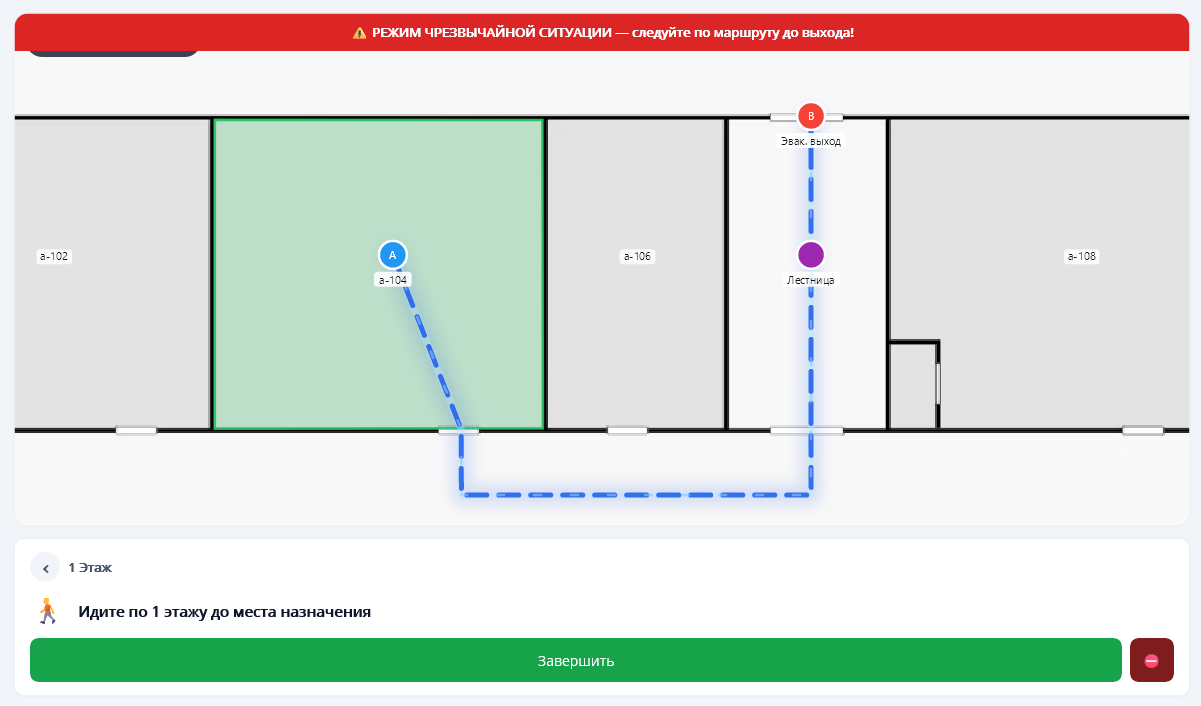
\includegraphics[width=0.95\textwidth]{Pictures/rpemergency.png}
\caption{Эвакуационный маршрут до ближайшего выхода в режиме ЧС}
\label{rpemergency:image}
\end{figure}

\subsubsection{Перестроение маршрута при блокировке}

\textbf{Сценарий.} Пользователь отмечает заблокированный узел на текущем маршруте, после чего система перестраивает путь.

\textbf{Результат.} Маршрут автоматически перестроен в обход заблокированного участка без перезагрузки графа. Результат подтверждает работу механизма динамического исключения узлов и показан на рисунке~\ref{rpreroute:image}.

\begin{figure}[H]
\centering
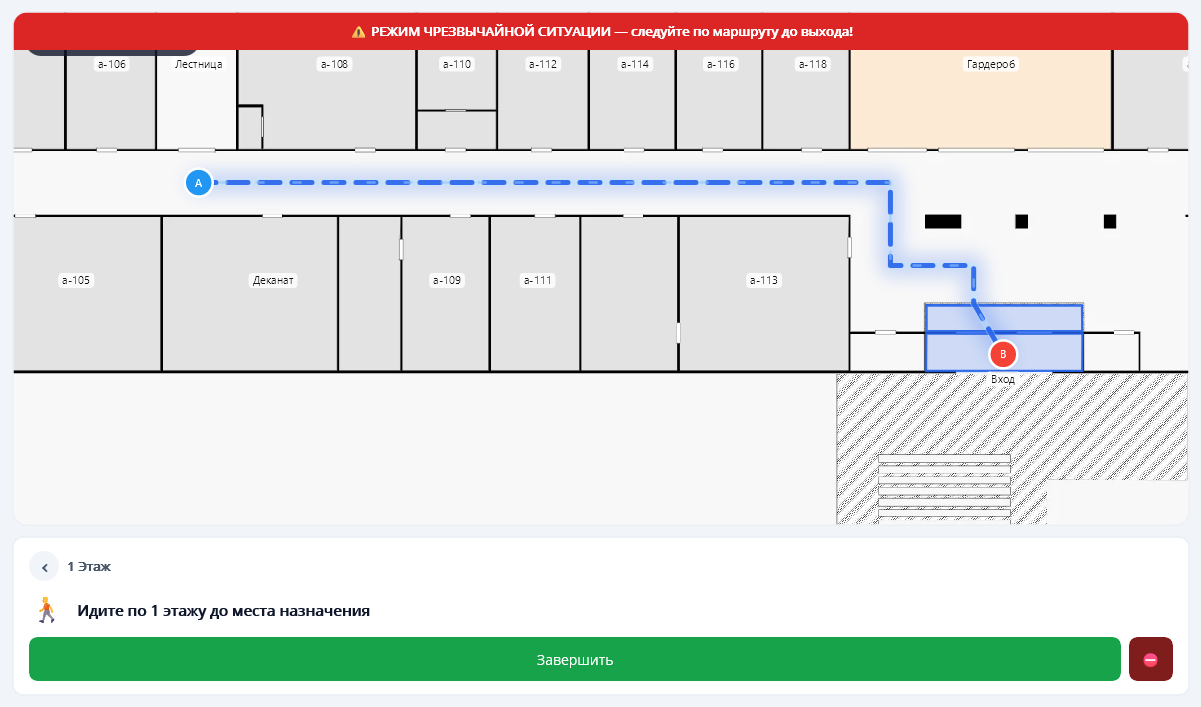
\includegraphics[width=0.95\textwidth]{Pictures/rpreroute.png}
\caption{Перестроение маршрута при блокировке участка}
\label{rpreroute:image}
\end{figure}

\subsubsection{Позиционирование пользователя по QR-коду}

\textbf{Сценарий.} Пользователь сканирует QR-код, размещённый на стене здания. Приложение разбирает ссылку вида \texttt{indoornav://node/\{id\}}, устанавливает соответствующий узел как начальную точку.

\textbf{Результат.} Начальная точка маршрута корректно определена по отсканированному QR-коду. Результат подтверждает интеграцию модуля разбора ссылок с алгоритмом маршрутизации и показан на рисунке~\ref{rpsys2:image}.

\begin{figure}[H]
	\centering
	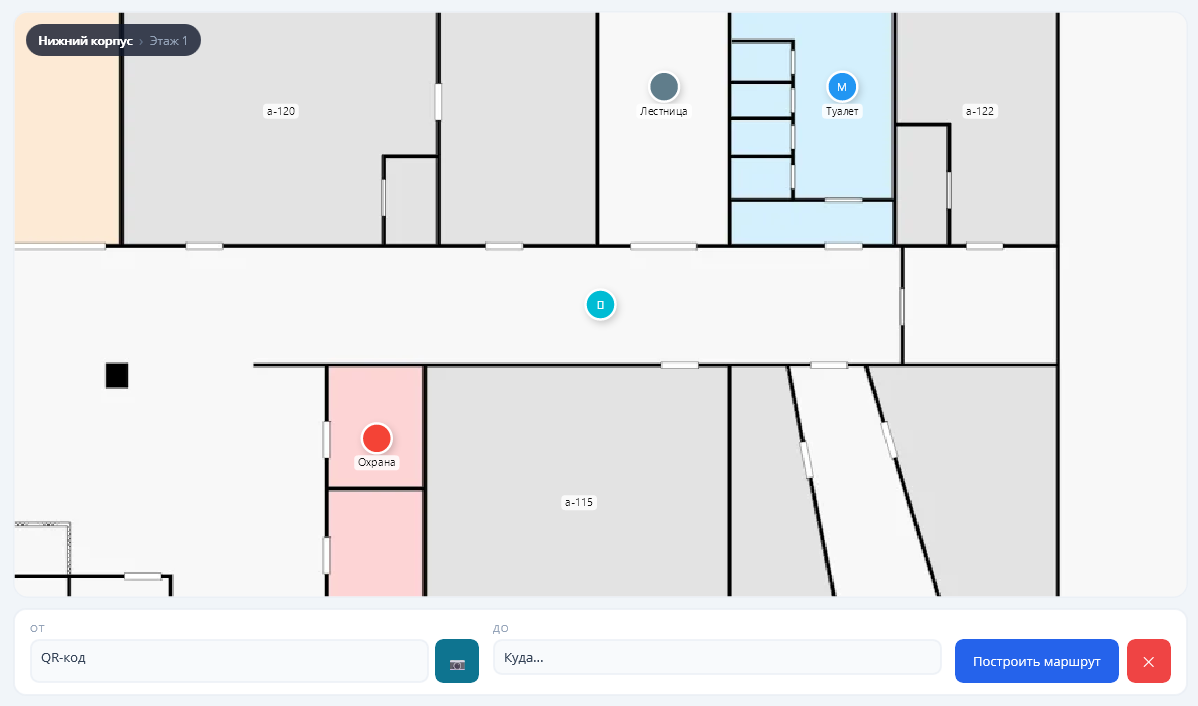
\includegraphics[width=0.95\textwidth]{Pictures/rpsys2.png}
	\caption{Позиционирование пользователя по QR-коду}
	\label{rpsys2:image}
\end{figure}

\subsubsection{Определение исходной точки по расписанию в режиме ЧС}

\textbf{Сценарий.} В здании активирован режим чрезвычайной ситуации. При входе студента в приложение система запрашивает подтверждение того, что он находится в аудитории согласно своему расписанию. При подтверждении эта аудитория автоматически устанавливается как исходная точка, и сразу строится маршрут до ближайшего эвакуационного выхода.

\textbf{Результат.} Исходная точка маршрута определена по подтверждённой аудитории из расписания без ручного выбора, эвакуационный маршрут до ближайшего выхода построен автоматически. Результат подтверждает совместную работу сервиса расписания и модуля эвакуационной маршрутизации и показан на рисунке~\ref{rpsys3:image}.

\begin{figure}[H]
	\centering
	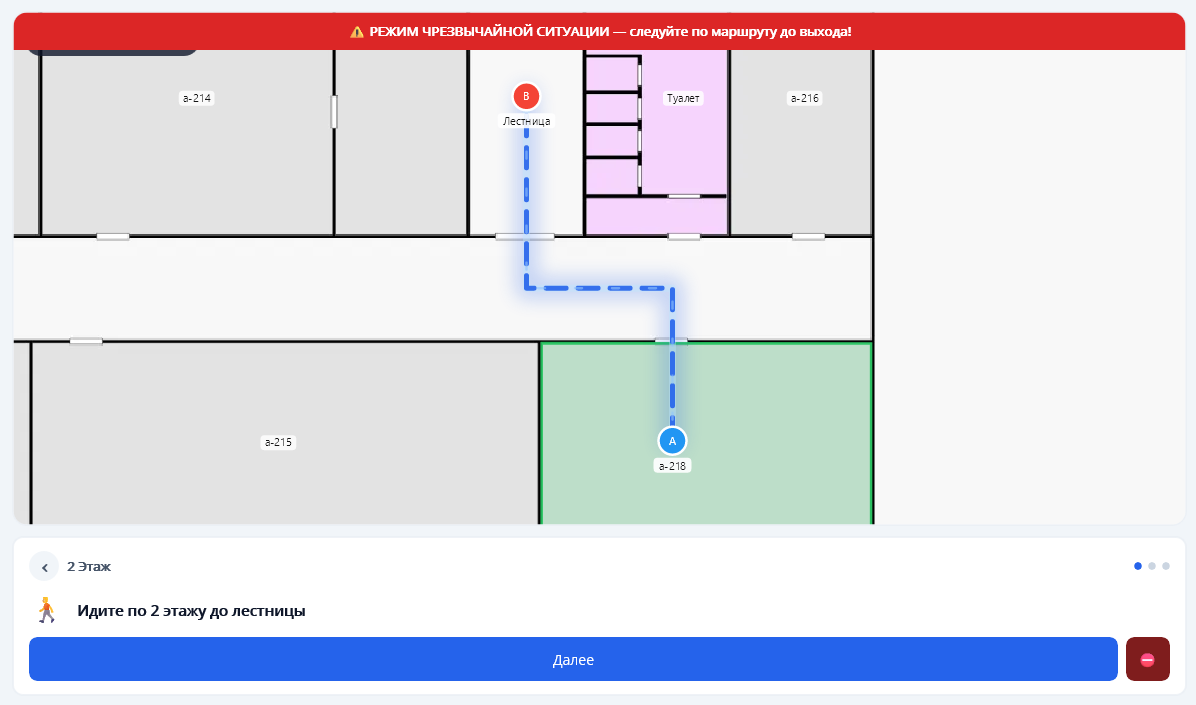
\includegraphics[width=0.95\textwidth]{Pictures/rpsys3.png}
	\caption{Определение исходной точки по расписанию в режиме ЧС}
	\label{rpsys3:image}
\end{figure}

Системное тестирование подтвердило корректную совместную работу всех слоёв приложения на реальных данных графа здания и на целевых платформах.


   % !TeX root = mainstarkov.tex
% !TeX program = xelatex
% !TeX encoding = UTF-8
\section*{ЗАКЛЮЧЕНИЕ}
\addcontentsline{toc}{section}{ЗАКЛЮЧЕНИЕ}

В рамках выпускной квалификационной работы выполнена программная реализация и тестирование алгоритмов динамической маршрутизации для системы построения эвакуационных маршрутов в замкнутых пространствах. Все поставленные задачи решены в полном объёме.

Проведён анализ существующих алгоритмов поиска кратчайших путей на графах. На основании сравнительного анализа по критериям оптимальности, производительности, поддержки динамического исключения узлов и сложности реализации выбран алгоритм Дейкстры как наилучшее решение для задачи эвакуационной маршрутизации. Алгоритм обеспечивает гарантию оптимальности при неотрицательных весах рёбер, эффективную работу на разреженных графах, характерных для планов зданий, и допускает модификацию для динамического исключения заблокированных узлов.

Разработаны структуры данных для представления навигационного графа: классы \texttt{NavGraph}, \texttt{NavNode} и \texttt{NavEdge}, обеспечивающие эффективное хранение и обработку топологии здания. Класс \texttt{NavNode} содержит полный набор атрибутов узла: координаты, номер этажа, идентификатор здания, флаги типа и группу перехода. Класс \texttt{NavEdge} хранит вес ребра с автоматическим вычислением евклидова расстояния для проходов. Реализована загрузка и сохранение графа в формате JSON средствами \texttt{System.Text.Json}.

Реализован алгоритм Дейкстры с модификациями для поддержки динамического исключения узлов. Множество исключённых узлов передаётся как параметр метода \texttt{FindPath} и проверяется при релаксации рёбер без модификации исходного графа. Конечный узел маршрута никогда не исключается. Алгоритм использует стандартные структуры данных .NET (\texttt{SortedSet}, \texttt{Dictionary}, \texttt{HashSet}) и обеспечивает время выполнения менее 200 мс для графов до 500 узлов, что соответствует требованиям реального времени. Оптимизация списка смежности и обработка устаревших записей очереди повышают эффективность реализации.

Разработан алгоритм поиска ближайшего эвакуационного выхода, учитывающий текущее положение пользователя, принадлежность к зданию и динамически изменяющиеся препятствия. Алгоритм приоритизирует выходы в текущем здании. Алгоритм интегрирован с сервисом экстренной эвакуации \texttt{EmergencyService} и ViewModel приложения IndoorNav.

Разработан механизм формирования множества исключённых узлов \texttt{BuildExcludeSet}, объединяющий заблокированные пользователем узлы и выходы, не являющиеся целевыми. Это предотвращает прохождение маршрута через другие выходы и обеспечивает корректное перестроение маршрута при блокировке участков.

Проведено комплексное тестирование алгоритмической части: модульное тестирование четырёх модулей маршрутизации (построение маршрута, поиск эвакуационного выхода, вычисление весов рёбер и формирование множества исключений), тестирование производительности на графах от 50 до 500 узлов, а также интеграционное тестирование на реальных данных графа здания университета. Результаты подтвердили корректность работы алгоритмов во всех сценариях, включая граничные случаи (пустой граф, несвязный граф, совпадение стартовой и конечной точек), и соответствие требованиям производительности.

Таким образом, в ходе выпускной квалификационной работы реализованы и верифицированы алгоритмы динамической маршрутизации для системы построения эвакуационных маршрутов в замкнутых пространствах. Полученные результаты могут быть применены в навигационных системах внутри зданий, приложениях экстренной эвакуации и иных программных комплексах, требующих эффективного построения маршрутов с учётом динамических ограничений. Дальнейшее развитие системы может включать реализацию алгоритма A* с допустимой эвристикой, поддержку двунаправленного поиска и интеграцию с серверной частью для распределённого построения маршрутов.

}\fi
\addcontentsline{toc}{section}{СПИСОК ИСПОЛЬЗОВАННЫХ ИСТОЧНИКОВ}

\begin{thebibliography}{99}
	
	%% ===== I. НОРМАТИВНЫЕ ДОКУМЕНТЫ =====
	
	\bibitem{gost19102} ГОСТ~19.102-77. Единая система программной документации. Стадии разработки. --- URL: \url{https://docs.cntd.ru/document/1200007652} (дата обращения: 07.05.2026).
	
	\bibitem{gost19105} ГОСТ~19.105-78. Единая система программной документации. Общие требования к программным документам. --- URL: \url{https://docs.cntd.ru/document/1200007655} (дата обращения: 07.05.2026).
	
	\bibitem{gost19201} ГОСТ~19.201-78. Единая система программной документации. Техническое задание. Требования к содержанию и оформлению. --- URL: \url{https://docs.cntd.ru/document/1200007659} (дата обращения: 07.05.2026).
	
	\bibitem{gost19301} ГОСТ~19.301-79. Единая система программной документации. Программа и методика испытаний. Требования к содержанию и оформлению. --- URL: \url{https://docs.cntd.ru/document/1200007663} (дата обращения: 07.05.2026).
	
	\bibitem{iso25010} ГОСТ~Р~ИСО/МЭК~25010-2015. Информационные технологии. Системная и программная инженерия. Требования и оценка качества систем и программного обеспечения (SQuaRE). Модели качества систем и программных продуктов. --- URL: \url{https://docs.cntd.ru/document/1200121069} (дата обращения: 07.05.2026).
	
	\bibitem{fz123} Федеральный закон от 22.07.2008 №~123-ФЗ «Технический регламент о требованиях пожарной безопасности». --- URL: \url{https://www.consultant.ru/document/cons_doc_LAW_78699/} (дата обращения: 07.05.2026).
	
	\bibitem{sp113130} СП~1.13130.2009. Системы противопожарной защиты. Эвакуационные пути и выходы. --- URL: \url{https://docs.cntd.ru/document/1200071143} (дата обращения: 07.05.2026).
	
	%% ===== II. ТЕХНИЧЕСКАЯ ДОКУМЕНТАЦИЯ =====
	
	\bibitem{json} Ecma International. The JSON Data Interchange Format. Standard ECMA-404, 2nd~ed. --- URL: \url{https://www.ecma-international.org/publications-and-standards/standards/ecma-404/} (дата обращения: 07.05.2026).
	
	\bibitem{maui} Microsoft. .NET Multi-platform App UI (MAUI) documentation. --- URL: \url{https://learn.microsoft.com/dotnet/maui/} (дата обращения: 07.05.2026).
	
	\bibitem{mauimvvm} Microsoft. Model-View-ViewModel (MVVM) in .NET MAUI. --- URL: \url{https://learn.microsoft.com/dotnet/maui/xaml/fundamentals/mvvm} (дата обращения: 07.05.2026).
	
	\bibitem{mauidi} Microsoft. Dependency injection in .NET MAUI. --- URL: \url{https://learn.microsoft.com/dotnet/maui/fundamentals/dependency-injection} (дата обращения: 07.05.2026).
	
	\bibitem{xaml} Microsoft. XAML overview in .NET MAUI. --- URL: \url{https://learn.microsoft.com/dotnet/maui/xaml/} (дата обращения: 07.05.2026).
	
	\bibitem{skiasharp} Microsoft. SkiaSharp graphics in .NET MAUI. --- URL: \url{https://learn.microsoft.com/dotnet/maui/user-interface/graphics/skiasharp/} (дата обращения: 07.05.2026).
	
	\bibitem{systemtextjson} Microsoft. System.Text.Json overview. --- URL: \url{https://learn.microsoft.com/dotnet/standard/serialization/system-text-json/overview} (дата обращения: 07.05.2026).
	
	\bibitem{navigineSdk} Navigine. Indoor Navigation and Positioning SDK Documentation. --- URL: \url{https://navigine.com/sdk-documentation/} (дата обращения: 07.05.2026).
	
	\bibitem{situmDocs} Situm Technologies. Situm Indoor Positioning Platform. Developer Documentation. --- URL: \url{https://situm.com/docs/} (дата обращения: 07.05.2026).
	
	\bibitem{mappedinDocs} Mappedin Inc. Mappedin Developer Documentation. --- URL: \url{https://developer.mappedin.com/docs/} (дата обращения: 07.05.2026).
	
	\bibitem{twogisFloors} 2ГИС. Поэтажные планы в MapGL JavaScript API. --- URL: \url{https://docs.2gis.com/ru/mapgl/reference/indoor} (дата обращения: 07.05.2026).
	
	\bibitem{mapstedOfficial} Mapsted Corp. Indoor Navigation Technology. --- URL: \url{https://mapsted.com/indoor-navigation/} (дата обращения: 07.05.2026).
	
	%% ===== III. РУССКОЯЗЫЧНЫЕ ИСТОЧНИКИ (39) =====
	
	\bibitem{amelichev2022} Амеличев~Г.Э., Панина~В.С. Сравнительный анализ алгоритмов поиска пути в помещении // E-Scio. --- 2022. --- URL: \url{https://cyberleninka.ru/article/n/sravnitelnyy-analiz-algoritmov-poiska-puti-v-pomeschenii} (дата обращения: 07.05.2026).
	
	\bibitem{cormen} Близнякова~Е.А., Куликов~А.А., Куликов~А.В. Сравнительный анализ методов поиска кратчайшего пути в графе // Архитектура, строительство, транспорт. --- 2022. --- Т.~1 (99). --- С.~80--87. --- DOI:~10.31660/2782-232X-2022-1-80-87.
	
	\bibitem{vinnikov2022} Виннников~М.Д. Разработка базы данных для мобильного приложения на операционной системе Android // Научные известия. --- 2022. --- URL: \url{https://cyberleninka.ru/article/n/razrabotka-bazy-dannyh-dlya-mobilnogo-prilozheniya-na-operatsionnoy-sisteme-android} (дата обращения: 07.05.2026).
	
	\bibitem{gof} Гамма~Э., Хелм~Р., Джонсон~Р., Влиссидес~Дж. Паттерны объектно-ориентированного проектирования / пер.~с~англ. --- СПб.~: Питер, 2021. --- 448~с. --- ISBN~978-5-4461-1595-2.
	
	\bibitem{gravit2019} Гравит~М.В., Карькин~И.Н., Дмитриев~И.И., Кузенков~К.А. Моделирование процесса эвакуации из высотных зданий и сооружений с использованием пассажирских лифтов // Пожаровзрывобезопасность. --- 2019. --- Т.~28, №~2. --- С.~66--80. --- DOI:~10.18322/PVB.2019.28.02.66-80.
	
	\bibitem{grinyak2018} Гриняк~В.М., Гриняк~Т.М., Цибанов~П.А. Позиционирование внутри помещений с помощью Bluetooth-устройств // Территория новых возможностей. Вестник ВГУЭС. --- 2018. --- Т.~10, №~2. --- С.~137--147. --- DOI:~10.24866/VVSU/2073-3984/2018-2/137-147.
	
	\bibitem{gusarova2023} Гусарова~А.А. Современные информационные технологии как инструмент повышения пожарной безопасности зданий // Пожаровзрывобезопасность. --- 2023. --- Т.~32, №~6. --- С.~36--46. --- DOI:~10.22227/0869-7493.2023.32.06.36-46.
	
	\bibitem{dijkstra} Гюллинг~А.О., Воронцова~Н.В. Визуализация алгоритма Дейкстры // Известия Тульского государственного университета. Технические науки. --- 2024. --- Т.~2. --- С.~127--128. --- DOI:~10.24412/2071-6168-2024-2-127-128.
	
	\bibitem{ershov2021} Ершов~Т.А. Обзор технологии мобильной разработки Xamarin // StudNet. --- 2021. --- URL: \url{https://cyberleninka.ru/article/n/obzor-tehnologii-mobilnoy-razrabotki-xamarin} (дата обращения: 07.05.2026).
	
	\bibitem{eskendir2019} Ескендир~М.А. Введение в разработку мобильных приложений // Вестник магистратуры. --- 2019. --- URL: \url{https://cyberleninka.ru/article/n/vvedenie-v-razrabotku-mobilnyh-prilozheniy} (дата обращения: 07.05.2026).
	
	\bibitem{zaitseva2021} Зайцева~И.А., Эбата~В.Ч., Ковбаса~Н.А. Практика применения методологий Agile, Scrum в ИТ-проектах // Индустриальная экономика. --- 2021. --- Т.~1. --- DOI:~10.47576/2712-7559\_2021\_1\_62.
	
	\bibitem{zhukovskaya2017} Жуковская~А.Н., Заушицина~А.С. Особенности разработки кроссплатформенных мобильных приложений // Решетнёвские чтения. --- 2017. --- URL: \url{https://cyberleninka.ru/article/n/osobennosti-razrabotki-krossplatformennyh-mobilnyh-prilozheniy} (дата обращения: 07.05.2026).
	
	\bibitem{levitin} Изотова~Т.Ю. Обзор алгоритмов поиска кратчайшего пути в графе // Новые информационные технологии в автоматизированных системах. --- 2016. --- URL: \url{https://cyberleninka.ru/article/n/obzor-algoritmov-poiska-kratchayshego-puti-v-grafe} (дата обращения: 07.05.2026).
	
	\bibitem{ilichev2018} Ильичёв~М.В., Мезенцева~Е.М. Фреймворк Xamarin // Теория и практика современной науки. --- 2018. --- URL: \url{https://cyberleninka.ru/article/n/freymvork-xamarin} (дата обращения: 07.05.2026).
	
	\bibitem{isaev2023} Исаев~М.И., Вахаева~Д.А., Алдамов~А.И. Алгоритмы для нахождения кратчайшего пути // Региональная и отраслевая экономика. --- 2023. --- №~4. --- С.~16--19. --- DOI:~10.47576/2949-1916\_2023\_4\_16.
	
	\bibitem{karmanova2020} Карманова~М.В. Концепция разработки мобильных приложений для картографирования зон чрезвычайных ситуаций и происшествий // Интерэкспо Гео-Сибирь. --- 2020. --- Т.~1, №~2. --- С.~68--74. --- DOI:~10.33764/2618-981X-2020-1-2-68-74.
	
	\bibitem{freeman} Кошелев~О.В. Шаблоны проектирования в программировании // Научный журнал. --- 2018. --- URL: \url{https://cyberleninka.ru/article/n/shablony-proektirovaniya-v-programmirovanii} (дата обращения: 07.05.2026).
	
	\bibitem{kulikov2021} Куликов~А.С. Обзор основных методов внутренней навигации // Форум молодых учёных. --- 2021. --- URL: \url{https://cyberleninka.ru/article/n/obzor-osnovnyh-metodov-vnutrenniy-navigatsii} (дата обращения: 07.05.2026).
	
	\bibitem{marinin2024} Маринин~А.К. Выбор архитектуры для мобильных приложений // Известия Кабардино-Балкарского НЦ РАН. --- 2024. --- Т.~26, №~5. --- С.~84--93. --- DOI:~10.35330/1991-6639-2024-26-5-84-93.
	
	\bibitem{fowler} Мартин~Р. Чистая архитектура. Искусство разработки программного обеспечения / пер.~с~англ. --- СПб.~: Питер, 2022. --- 352~с. --- ISBN~978-5-4461-0772-8.
	
	\bibitem{mongush2017} Монгуш~А.В., Кикин~П.М. Обзор технологий indoor-навигации // Интерэкспо Гео-Сибирь. --- 2017. --- URL: \url{https://cyberleninka.ru/article/n/obzor-tehnologiy-indoor-navigatsii} (дата обращения: 07.05.2026).
	
	\bibitem{naumov2021} Наумов~Р.К., Железков~Н.Э. Сравнительный анализ форматов хранения текстовых данных для дальнейшей обработки методами машинного обучения // Научный результат. Информационные технологии. --- 2021. --- Т.~6, №~1. --- С.~40--47. --- DOI:~10.18413/2518-1092-2021-6-1-0-5.
	
	\bibitem{ohotichenko2021} Охотиченко~А.В., Ухта~Ю.Б. Проектирование системы для навигации внутри здания со сложной иерархической структурой // Программные системы и вычислительные методы. --- 2021. --- №~4. --- С.~46--57. --- DOI:~10.7256/2454-0714.2021.4.37012.
	
	\bibitem{sazonov2024} Сазонов~А.П. Использование принципа Dependency Injection в мобильной разработке // Инновации и инвестиции. --- 2024. --- URL: \url{https://cyberleninka.ru/article/n/ispolzovanie-printsipa-dependency-injection-v-mobilnoy-razrabotke-na-territorii-rb} (дата обращения: 07.05.2026).
	
	\bibitem{samoshin2026} Самошин~Д.А., Георгиев~Н.А., Климовцова~Я.О., Кочетыгов~В.А. Затраты времени на изучение плана эвакуации и рекомендации по повышению его эффективности // Пожары и чрезвычайные ситуации: предотвращение, ликвидация. --- 2026. --- №~1. --- С.~26--36. --- DOI:~10.25257/FE.2026.1.26-36.
	
	\bibitem{albahari} Сергеев~К.С., Афонин~А.Ю., Осин~С.М. Особенности и различия архитектурных паттернов MV в языке программирования C\# // Парадигма. --- 2025. --- №~4. --- Ч.~2. --- URL: \url{https://cyberleninka.ru/article/n/osobennosti-i-razlichiya-arhitekturnyh-patternov-mv-v-yazyke-programmirovaniya-c} (дата обращения: 07.05.2026).
	
	\bibitem{sterlyagov2017} Стерлягов~С.П., Селютина~Е.П. Применение User Experience/User Interface моделирования для разработки мобильного приложения // Международный научно-исследовательский журнал. --- 2017. --- Т.~62. --- DOI:~10.23670/IRJ.2017.62.067.
	
	\bibitem{zhang2015} Ткачев~Д.В. Графы и их применение при чрезвычайных ситуациях // Вестник науки и образования. --- 2019. --- URL: \url{https://cyberleninka.ru/article/n/grafy-i-ih-primenenie-pri-chrezvychaynyh-situatsiyah} (дата обращения: 07.05.2026).
	
	\bibitem{richter} Троелсен~Э., Джепикс~Ф. Язык программирования C\#~7 и платформы .NET и .NET Core / пер.~с~англ. --- М.~: Диалектика, 2018. --- 1328~с. --- ISBN~978-5-6040723-1-8.
	
	\bibitem{uvarov2016} Уваров~А.Н. Инверсия управления и внедрение зависимостей // Символ науки. --- 2016. --- №~10-1. --- URL: \url{https://cyberleninka.ru/article/n/inversiya-upravleniya-i-vnedrenie-zavisimostey} (дата обращения: 07.05.2026).
	
	\bibitem{urbanovich2023} Урбанович~М.В., Ковалева~К.А. Принципы разработки пользовательских интерфейсов // Современные инновации, системы и технологии. --- 2023. --- Т.~3, №~4. --- DOI:~10.47813/2782-2818-2023-3-4-0363-0374.
	
	\bibitem{feshina2022} Фешина~Е.В., Пчела~Д.В., Долгов~А.В., Трофимов~Д.И. Анализ технологий разработки мобильных приложений и информационных систем на базе ОС Android // Вестник Адыгейского государственного университета. Сер.~4. --- 2022. --- Т.~1 (296). --- С.~85--91. --- DOI:~10.53598/2410-3225-2022-1-296-85-91.
	
	\bibitem{yarovaya2022} Яровая~Е.В. Принципы построения архитектуры программного обеспечения // E-Scio. --- 2022. --- URL: \url{https://cyberleninka.ru/article/n/printsipy-postroeniya-arhitektury-programmnogo-obespecheniya} (дата обращения: 07.05.2026).
	
	%% ===== IV. ИНОСТРАННЫЕ ИСТОЧНИКИ (11) =====
	
	\bibitem{deng2021} Deng~H., Ou~Z., Zhang~G., Deng~Y., Tian~M. BIM and Computer Vision-Based Framework for Fire Emergency Evacuation Considering Local Safety Performance // Sensors. --- 2021. --- Vol.~21, No.~11. --- Art.~3851. --- DOI:~10.3390/s21113851.
	
	\bibitem{han2020} Han~L., Guo~H., Zhang~H., Kong~Q., Zhang~A., Gong~C. An Efficient Staged Evacuation Planning Algorithm Applied to Multi-Exit Buildings // ISPRS International Journal of Geo-Information. --- 2020. --- Vol.~9, No.~1. --- Art.~46. --- DOI:~10.3390/ijgi9010046.
	
	\bibitem{jia2018} Jia~X., Ebone~A., Tan~Y. A Performance Evaluation of Cross-Platform Mobile Application Development Approaches // Proceedings of the 5th IEEE/ACM International Conference on Mobile Software Engineering and Systems (MOBILESoft~2018). --- Gothenburg, 2018. --- P.~92--93. --- DOI:~10.1145/3197231.3197252.
	
	\bibitem{landau2020} Landau~Y., Ben-Moshe~B. STEPS: An Indoor Navigation Framework for Mobile Devices // Sensors. --- 2020. --- Vol.~20, No.~14. --- Art.~3929. --- DOI:~10.3390/s20143929.
	
	\bibitem{mirahadi2020} Mirahadi~F., McCabe~B.Y. EvacuSafe: Building Evacuation Strategy Selection Using Route Risk Index // Journal of Computing in Civil Engineering (ASCE). --- 2020. --- Vol.~34, No.~2. --- Art.~04019051. --- DOI:~10.1061/(ASCE)CP.1943-5487.0000867.
	
	\bibitem{mirahadi2021} Mirahadi~F., McCabe~B.Y. EvacuSafe: A Real-Time Model for Building Evacuation Based on Dijkstra's Algorithm // Journal of Building Engineering. --- 2021. --- Vol.~34. --- Art.~101687. --- DOI:~10.1016/j.jobe.2020.101687.
	
	\bibitem{rubio2021} Rubio-Sandoval~J.I., Martínez-Rodríguez~J.-L., Lopez-Arevalo~I., Ríos-Alvarado~A.B., Rodríguez-Rodríguez~A.J., Vargas-Requena~D.T. An Indoor Navigation Methodology for Mobile Devices by Integrating Augmented Reality and Semantic Web // Sensors. --- 2021. --- Vol.~21, No.~16. --- Art.~5435. --- DOI:~10.3390/s21165435.
	
	\bibitem{singh2021} Singh~N., Choe~S., Punmiya~R. Machine Learning Based Indoor Localization Using Wi-Fi RSSI Fingerprints: An Overview // IEEE Access. --- 2021. --- Vol.~9. --- P.~127150--127174. --- DOI:~10.1109/ACCESS.2021.3111083.
	
	\bibitem{tomazic2021} Tomažič~S. Indoor Positioning and Navigation // Sensors. --- 2021. --- Vol.~21, No.~14. --- Art.~4793. --- DOI:~10.3390/s21144793.
	
	\bibitem{yen2021} Yen~H.-H., Lin~C.-H., Tsao~H.-W. Time-Aware and Temperature-Aware Fire Evacuation Path Algorithm in IoT-Enabled Multi-Story Multi-Exit Buildings // Sensors. --- 2021. --- Vol.~21, No.~1. --- Art.~111. --- DOI:~10.3390/s21010111.
	
	\bibitem{zhangfire2019} Zhang~J., Guo~J., Xiong~H., Liu~X., Zhang~D. A Framework for an Intelligent and Personalized Fire Evacuation Management System // Sensors. --- 2019. --- Vol.~19, No.~14. --- Art.~3128. --- DOI:~10.3390/s19143128.
	
\end{thebibliography}

\ifВКР{\appendix{Представление графического материала}

Графический материал, выполненный на отдельных листах,
изображен на рисунках А.1--А.\arabic{числоПлакатов}.
\setcounter{числоПлакатов}{0}

\renewcommand{\thefigure}{А.\arabic{figure}} % шаблон номера для плакатов

\begin{landscape}
	
	\begin{плакат}
		\includegraphics[width=0.82\linewidth]{плакат1.eps}
		\заголовок{Сведения о ВКРБ}
		\label{pl1:image}      
	\end{плакат}
	
	\begin{плакат}
		\includegraphics[width=0.82\linewidth]{плакат2.eps}
		\заголовок{Цель и задачи разработки}
		\label{pl2:image}      
	\end{плакат}
	
	\begin{плакат}
		\includegraphics[width=0.82\linewidth]{плакат3.eps}
		\заголовок{Диаграмма вариантов использования}
		\label{pl3:image}      
	\end{плакат}
	
	\begin{плакат}
		\includegraphics[width=0.82\linewidth]{плакат4.eps}
		\заголовок{Концептуальная модель программы}
		\label{pl4:image}      
	\end{плакат}
	
	\begin{плакат}
		\includegraphics[width=0.82\linewidth]{плакат5.eps}
		\заголовок{Построение маршрута между аудиториями}
		\label{pl5:image}      
	\end{плакат}
	
	\begin{плакат}
		\includegraphics[width=0.82\linewidth]{плакат6.eps}
		\заголовок{Время построения маршрута в зависимости от размера графа}
		\label{pl6:image}      
	\end{плакат}
	
	\begin{плакат}
		\includegraphics[width=0.82\linewidth]{плакат7.eps}
		\заголовок{Процесс построения маршрута по слояим приложения}
		\label{pl7:image}      
	\end{плакат}
	
	\begin{плакат}
		\includegraphics[width=0.82\linewidth]{плакат8.eps}
		\заголовок{Заключение}
		\label{pl8:image}      
	\end{плакат}
\end{landscape}
}\fi
\ifПрактика{}\else{\input{Код}}\fi
\end{document}
